% !TeX document-id = {d6880f2a-54da-4cb0-a23a-f83a328218ac}
% !TeX program = xelatex
% !BIB program = biber

%Document vide aux normes de l'École nationale des Chartes
%crée par J.B. Camps
%Dernières modifications E. Rouquette (03/2026)

%%%%%%%%%%%%%%%%%%%%%% PRÉAMBULE


%%%%%%%%%%%%%% partie obligatoire du préambule
\documentclass[12pt,twoside]{book}
\usepackage{fontspec}
\usepackage{xunicode}
\usepackage[french]{babel}
\usepackage{pdfpages} % Inserer les pdf en entier
\usepackage{float} % Ajout de l'option position H pour les figures et les tableaux
\usepackage{enumitem} % Pour citer sous la forme de tirets des idées 
\usepackage{booktabs} % Commande pour avoir des tableaux plus soignés



\usepackage[acronym]{glossaries}
\makeglossaries

%%%%%%%%%%%%%% Pour la liste des abréviations

\newacronym{AMO}{AMO}{Assistance à maîtrise d’ouvrage}
\newacronym{api}{API}{Application Programming Interface}
\newacronym{bad}{BAD}{Bibliothèque-Archives-Documentation}
\newacronym{cci}{CCI}{Centre de création industrielle} 
\newacronym{diaman}{DIAMAN}{Dispositif Interministériel D'Accompagnement des Missions pour l'Archivage Numérique}
\newacronym{droid}{DROID}{Digital Record Object Identification}
\newacronym{mad}{MAD}{Musée des Arts Décoratifs}
\newacronym{mets}{METS}{Metadata Encoding and Transmission Standard}
\newacronym{oais}{OAIS}{Open Archival Information System}
\newacronym{pronom}{PRONOM}{Public Record Office and Nôm}
\newacronym{sae}{SAE}{Système d'Archivage Électronique}
\newacronym{seda}{SEDA}{Standard d'Echange de Données pour le d'Archivage}
\newacronym{siaf}{SIAF}{Service interministériel des Archives de France}
\newacronym{sip}{SIP}{Submission Information Package}
\newacronym{vas}{VaS}{Vitam Accessible en Service}
\newacronym{vitam}{VITAM}{Valeurs Immatérielles Transmises aux Archives pour la Mémoire}
\newacronym{ucad}{UCAD}{Union Centrale des Arts Décoratifs}
\newacronym{ucbaai}{UCBAAI}{Union Centrale des Beaux-Arts Appliqués à l'Industrie}


%\usepackage{polyglossia}
%\setotherlanguage{} %indiquer les autres langues utilisée


%%%%%%%%%%%%%%%%%%%%%%%%%%%%%%%%% PACKAGES UTILISÉS

\usepackage{csquotes} % les guillemets français
\usepackage{lettrine} %faire une lettrine (pas obligatoire)
\usepackage[backend=biber,style=enc,sorting=nyt,maxbibnames=10,language=french
]{biblatex}
\addbibresource{bibliographie.bib}%charger le style de l'EnC (téléchargeable ici https://ctan.org/pkg/biblatex-enc)
% Répéter le numéro de page même après Ibid.
\ExecuteBibliographyOptions{ibidpage=false} % repère le numéro de la page après le Ibid
% Ajustement du rendu des articles des périodiques selon les normes de l'ENC car nous avons eu un problème à ce niveau
\renewbibmacro*{journal+issuetitle}{%
	\printtext{dans\space}% Ajout du mot "dans" avant le titre de la revue
	\usebibmacro{journal}% Affiche le titre de la revue propre à l'ENC
	\iffieldundef{number}% Si le numéro de la revue est renseigner, on le relève
	{}
	{\setunit{\addcomma\space}% Ajout d'une virgule après le titre de la revue
		\printtext{n°}\printfield{number}}% Affichage du numéro suivi de la revue
	\setunit{\addspace}%Ajout d'un espace après l'année
	\mkbibparens{\printfield{year}}% Affichage de l'année entre parenthèse
	\newunit %Fin de l'unité bibliographie et affichage des éléments suivants
}



%%%Faire un ou plusieurs index

%\usepackage{imakeidx} %pour faire un ou plusieurs index
%\makeindex %commande pour générer l'index


%RAJOUTEZ ICI VOS PACKAGES

% ---------- FIGURES ET GRAPHIQUES ----------
\usepackage{graphicx} % Insérer des images et graphiques
\usepackage{float} % Permet notamment d'utiliser [H] pour fixer une figure
\usepackage{placeins} % Permet d'utiliser \FloatBarrier pour contrôler les flottants



% ---------- COULEURS ----------
\usepackage[table]{xcolor} % Couleurs dans le texte, figures et tableaux

% ---------- TABLEAUX ----------
\usepackage{booktabs} % Tableaux plus propres : \toprule, \midrule, \bottomrule
\usepackage{tabularx} % Tableaux adaptés à la largeur de la page
\usepackage{longtable} % Tableaux qui s'étendent sur plusieurs pages
\usepackage{makecell} % Mise en forme des cellules et retours à la ligne
\usepackage{tablefootnote} % Notes de bas de page dans les tableaux
\usepackage{pdflscape} % Pages en paysage pour les grands tableaux

% ---------- CODE ----------
\usepackage{listings} % Présentation et coloration syntaxique du code

% ---------- TYPOGRAPHIE ----------
\usepackage{microtype} % Pour un visuel esthétique

% ---------- PDF ----------
\usepackage{pdfpages} % Insérer des pages PDF, notamment dans les annexes



%%%%%%%%%%%%%%%%%%%%%%%%%%%%%%%%% CONFIGURATION DE MISE EN PAGE

%%%%%% Les compteurs (sections, subsections, etc)



\renewcommand{\thechapter}{\arabic{chapter}} %chapitre en chiffres arabes
\renewcommand{\thesection}{\thechapter.\arabic{section}.} %section numérotée en fonction du chapitre : 1.1., 1.2., 1.3., etc.
\renewcommand{\thesubsection}{\arabic{subsection}.}%subsection en chiffres arabes
\renewcommand{\thesubsubsection}{\alph{subsubsection}.}%subsubsection en lettres minuscules
\setcounter{tocdepth}{1} %Si l'on veut faire apparaître les subsubsection dans le table des matières (à commenter sinon)
\setcounter{secnumdepth}{1} %Les titres internes seront appelés avec \subsection*{} et ne seront donc pas numérotés.


%%%%%  Configurer le document selon les normes de l'école


\usepackage[margin=2.5cm]{geometry} %marges
\usepackage{setspace}
\geometry{margin=2.5cm}
\onehalfspacing % interligne de 1.5
\setlength\parindent{1cm} % indentation des paragraphes à 1 cm
\usepackage{minted} % Pour les blocs de code en couleur


%%%%% Mise en forme des headers (haut de page)

\usepackage{fancyhdr} %package utilisé pour modifier les headers
\pagestyle{fancy} %utiliser ses propres choix de mise en page et non ceux par défaut du package

\setlength\headheight{16pt}%la hauteur des headers

%%la façon dont les sections apparaissent dans les en-tête:

%\renewcommand{\sectionmark}[1]{\markright{\small\textit{\thesection~\  #1}}}%Faire apparaître dans les headers les sections en  petit et en italiques
\renewcommand{\sectionmark}[1]{}%Commenter la lign précédetne et mettre celle-ci pour ne pas avoir le titre des sections dans le header

%% réglages propres à frontmatter

\appto\frontmatter{\pagestyle{fancy}%
	\renewcommand{\chaptermark}[1]{\markboth{\small\textit{#1}}{}}% ne pas faire apparaître de <<numéro>> de chapitre dans les chapitres non numérotés (front: l'introduction, els remerciement, etc)
}

%% réglages propres à mainmatter

\appto\mainmatter{
\renewcommand{\chaptermark}[1]{\markboth{\small\chaptername~\thechapter~--\ \textit{#1}}{}}%faire apparaître dans les headers les sections en  petit et en italiques
%\renewcommand{\chaptermark}[1]{}%Commenter la ligne précédente et mettre celle-ci pour ne pas avoir le titre des chapitres  dans le header
}

%% réglages propres aux annexes

\appto\appendix{
	\renewcommand{\chaptermark}[1]{\markboth{\small~Annexe \thechapter~--\ \textit{#1}}{}}%faire apparaître dans les headers le nom des annexes
	%\renewcommand{\chaptermark}[1]{}%Commenter la ligne précédente et mettre celle-ci pour ne pas avoir le titre des chapitres  dans le header
}


%indiquer des règles d'hyphénation pour des mots précis si besoin
%\begin{hyphenrules}{french}
%	\hyphenation{}
%\end{hyphenrules}


%%%%%%% Package hyperref

% A mettre après les autres appels de packages car redéfinit certaines commandes).

\usepackage[colorlinks=false, breaklinks=true, pdfusetitle, pdfsubject ={Mémoire HN}, pdfkeywords={les mots-clés}]{hyperref} %
\usepackage[numbered]{bookmark}%va avec hyperref; marche mieux pour les signets. l'option numbered: les signets dans le pdf sont numérotés

% Compléter pdfsubjet et pdfkeywords
%Explication des options de hyperref (modifiables)
% hyperindex=false
% colorlinks=false: pour que le cadre des liens n'apparaisse pas à l'impression
% breaklinks permet d'avoir des liens allant sur pusieurs lignes
%pdfusetitle: utiliser \author et \title pour produire le nom et le titre du pdf


%avec overleaf, utiliser :
%\usepackage[xetex]{hyperref}
%\hypersetup{
	%	pdfauthor = {Prénom Nom},
	%	pdftitle = {titre},
	%	pdfsubject = {sujet},
	%	pdfkeywords = {premier mot-clé} {deuxième mot-clé} {troisième mot-clé} {etc}
	%}



%%%%%%%%%%%%%%%%%%%% Package glossaries

%Exception: il faut le charger APRÈS hyperref
%\usepackage[toc=true]{glossaries}
%\makeglossaries
%avec TexStudio: F9 pour compiler le glossaire (s'il y a aussi un index)

%mettre les entrées du glossaire ici ou les mettre dans un fichier à part que l'on appelle ici par \loadglsentries{nom_du_fichier.tex}

%Structure d'une entrée de glossaire
%\newglossaryentry{}{%
%	name={},%
%	description={}
%}


%%%%%%%%%%%%%%%%%% DÉFINITION DES COMMANDES ET ENVIRONNMENTS


 %%%%%%%%%%%%%% INFORMATIONS POUR LA PAGE DE TITRE
 
\author{Léticia \textsc{Mvogo} - M2 TNAH}
\title{Traitement automatisé d'un fonds d'archives numériques. Cas des dossiers d'expositions du Musée des Arts Décoratifs}

%%%%%%%%%%%%%%%%%%%%%% DOCUMENT
\begin{document}
	\begin{titlepage}
		\begin{center}
			
			\bigskip
			
			\begin{large}				
				ÉCOLE NATIONALE DES CHARTES\\
				UNIVERSITÉ PARIS, SCIENCES \& LETTRES
			\end{large}
			\begin{center}\rule{2cm}{0.02cm}\end{center}
			
			\bigskip
			\bigskip
			\bigskip
			\begin{Large}
				\textbf{Léticia Mvogo}\\
			\end{Large}
		%selon le cas
			\begin{normalsize} \textit{licencié.e ès d'archivistique }\\
				\textit{diplômé.e de master}
			\end{normalsize}
			
			\bigskip
			\bigskip
			\bigskip
			
			\begin{Huge}
				\textbf{Traitement automatisé d'un fonds d'archives numériques }\\
			\end{Huge}
			\bigskip
			\bigskip
			\begin{LARGE}
				\textbf{Cas des dossiers d'exposition du Musée des Arts Décoratifs}\\
			\end{LARGE}
			
			\bigskip
			\bigskip
			\bigskip
			\begin{large}
				Sous la direction de \textbf{Julien Fenech}
			\end{large}
			\vfill
			
			\begin{large}
				Mémoire 
				pour le diplôme de master \\
				\enquote{Technologies numériques appliquées à l'histoire} \\
				\bigskip
				2026
			\end{large}
			
		\end{center}
	\end{titlepage}

	\thispagestyle{empty}	
	\cleardoublepage
	
\frontmatter

	\chapter{Résumé}
\medskip
	\lettrine{L}{es} institutions patrimoniales sont aujourd'hui de plus en plus confrontées aux problématiques d'accumulation des documents numériques dans les espaces de stockage. Cette situation rend l'accès à l'information difficile : elles se retrouvent donc face au phénomène de vrac numérique. Le présent mémoire, réalisé à la suite de 12 mois d'alternance au sein des Arts décoratifs (MAD), ce mémoire se propose de présenter une chaîne de traitement automatisé appliquée aux dossiers d'exposition. Il permet de constater le rapport de complémentarité qu'il existe entre l'automatisation et le traitement archivistique. Son but est donc de structurer la masse documentaire, de garantir la pérennité, la sécurité et la valorisation des archives numériques de l'institution. \\
	
	\textbf{Mots-clés:} ~Accès à l'information~; vrac numérique~; Musée des Arts décoratifs~; automatisation~; chaîne de traitement~; traitement archivistique~; masse documentaire~; pérennité~; sécurité~; valorisation des archives numériques~; archives numériques.
	
	\textbf{Informations bibliographiques:} Léticia Mvogo, \textit{Traitement automatisé d'un fonds d'archives numériques. Cas des dossiers d'expositions du Musée des Arts Décoratifs}, mémoire de master \enquote{Technologies numériques appliquées à l'histoire}, dir. Julien Fenech, École nationale des chartes, 2026.
	
		\newpage{\pagestyle{empty}\cleardoublepage}
	
	\chapter{Remerciements}
	
\lettrine{J}e tiens à remercier sincèrement les personnes qui ont contribué de près ou de loin à l'accomplissement de ce travail.

Mes remerciements vont tout d'abord à Marie Dion, archiviste aux Arts décoratifs mais également ma tutrice durant mes douze mois d'alternance au sein de l'équipe Archives. Je la remercie pour son accueil, sa confiance pour me permettre de travailler sur un tel projet, pour son suivi, ses conseils ainsi que la relecture de mes travaux. 

Je remercie également toute l'équipe du Département Bibliothèque-Documentation-Archives pour leur accueil chaleureux et les échanges professionnels enrichissants. 

Mes remerciements s'adressent aussi à Edouard Vasseur pour la présidence du jury de ma soutenance. Je remercie aussi Julien Fenech, en la qualité de directeur du présent mémoire pour son suivi, ses conseils et pour le suivi de mes travaux. Je tiens également à exprimer ma gratitude à l'égard d'Emmanuelle Bermès pour ses conseils et ses relectures.

Je n'oublie pas ma promotion \enquote{d'Archi-potes}, déjà pour leur motivation et leur engagement quant à ces deux années de travail intense, ainsi que pour cette belle ambiance qui a contribué à une harmonie remarquable tout au long de cette formation. 

Je remercie enfin ma famille, mes amis en particulier Chloe Chaplot et Chiara Bonsignore pour leur soutien quelques fois muet mais d'un grand réconfort, surtout lors de la rédaction de ce travail.
	\newpage{\pagestyle{empty}\cleardoublepage}
	
%%%%%%%%%% Liste des Abréviation %%%%%%%%%

\chapter{Liste des abréviations}

\begin{center}
	\renewcommand{\arraystretch}{1.3}
	\begin{tabular}{@{}ll@{}}
		\textbf{AMO}    & Assistance à maîtrise d’ouvrage \\
		\textbf{API}    & Application Programming Interface \\
		\textbf{BAD}    & Bibliothèque-Archives-Documentation \\
		\textbf{CCI}    & Centre de création industrielle \\
		\textbf{DIAMAN} & Dispositif interministériel d’accompagnement des missions pour l’archivage numérique \\
		\textbf{DROID}  & Digital Record Object Identification \\
		\textbf{MAD}    & Musée des Arts Décoratifs \\
		\textbf{METS}   & Metadata Encoding and Transmission Standard \\
		\textbf{OAIS}   & Open Archival Information System \\
		\textbf{PRONOM}   & Public Record Office and Nôm \\
		\textbf{SAE}    & Système d’archivage électronique \\
		\textbf{SEDA}   & Standard d’échange de données pour l’archivage \\
		\textbf{SIAF}   & Service interministériel des Archives de France \\
		\textbf{SIP}    & Submission Information Package \\
		\textbf{VaS}    & Vitam accessible en service \\
		\textbf{VITAM}  & Valeurs Immatérielles Transmises aux Archives Pour Mémoire \\
		\textbf{UCAD}   & Union Centrale des Arts Décoratifs \\
		\textbf{UCBAAI} & Union Centrale des Beaux-Arts Appliqués à l’Industrie
	\end{tabular}
\end{center}


	
%%%%%%%%%%%% \bibliographie ici (normes de l'EnC)
%\printbibliography

%%%%%%%%%%%% Bibliographie

\nocite{*}

\chapter{Bibliographie}

% Définition des niveaux de titres utilisés dans la bibliographie
\defbibheading{firstlevel}{\section*{#1}}
\defbibheading{secondlevel}{\subsection*{#1}}
\defbibheading{thirdlevel}{\subsubsection*{#1}}


% =========================================================
% SOURCES PRIMAIRES
% =========================================================

\section*{Sources primaires}

\printbibliography[
keyword=archivesMADserieA,
title={Série A : Archives statutaires de l'UCAD (1861--1993)},
heading=secondlevel
]

\printbibliography[
keyword=rapportsActivite,
title={Rapports d'activités},
heading=secondlevel
]

\printbibliography[
keyword=archivesInternes,
title={Archives et documents d'activités de la Bibliothèque des Arts décoratifs (non classées, documents internes)},
heading=secondlevel
]


% =========================================================
% SOURCES SECONDAIRES
% =========================================================

\section*{Sources secondaires}

\printbibliography[
keyword=ouvrages,
title={Ouvrages},
heading=secondlevel
]

\printbibliography[
keyword=articles,
title={Articles},
heading=secondlevel
]

\printbibliography[
keyword=litteratureGrise,
title={Littérature grise},
heading=secondlevel
]


% =========================================================
% CADRE RÉGLEMENTAIRE ET NORMATIF
% =========================================================

\section*{Cadre réglementaire et normatif}

\printbibliography[
keyword=reglementationEuropeenne,
title={Réglementation européenne},
heading=secondlevel
]

\printbibliography[
keyword=reglementationFrancaise,
title={Réglementation française},
heading=secondlevel
]

\printbibliography[
keyword=normes,
title={Normes archivistiques},
heading=secondlevel
]


% =========================================================
% SOURCES NUMÉRIQUES
% =========================================================

\section*{Sources numériques}

\printbibliography[
keyword=sourcesNumeriques,
heading=none
]
	
\chapter{Introduction}	
\begin{displayquote}
	\textit{\enquote{Nul pouvoir politique sans contrôle de l'archive, sinon de la mémoire.La démocratisation effectivement se mesure toujours à ce critère essentiel : la participation et l'accès à l'archive, à sa constitution et à son interprétation.}}
	
	\par 
	Jacques Derrida\footnote{\cite{derrida-1995}. p. 11.} \\[0.2cm]
\end{displayquote}




Par cette affirmation, l'auteur nous rappelle que l'archive ne se limite pas à un simple dépôt documentaire. Celle-ci se situe bien au-delà de cette compréhension. Elle constitue le lieu où s'élabore la mémoire individuelle, collective et institutionnelle. Sa valeur ne réside donc pas seulement dans le document lui-même, mais également dans le contexte qui l’a vu naître, dans les relations qu’il entretient avec les autres documents constitutifs d’un fonds. Ce constat renvoie au principe fondamental du respect des fonds, en ce sens qu’un document ne peut être compris s’il n’est pas lié à son contexte de production, à sa provenance et aux relations organiques qui le lient aux autres documents produits dans le cadre d’une même activité.

Cette dimension contextuelle revêt une importance particulière au sein des institutions patrimoniales, dont la mission ne se réduit pas seulement à conserver des objets, mais également à préserver les connaissances qui permettent de les comprendre, de les documenter et de les transmettre. Le musée apparaît en ce sens comme un espace de recherche, de production et de diffusion des savoirs, bien au-delà de sa fonction d’exposition des collections. L’exercice de ces missions scientifiques s’accompagne d’une importante production documentaire, qui constitue le support de ses activités de conservation, d’étude et d’exposition\footnote{\cite{maze-2017}}. Cette perception trouve sa confirmation dans la définition adoptée par le Conseil international des musées (ICOM) en 2022, qui présente le musée comme \textit{\enquote{une institution permanente, à but non lucratif et au service de la société, qui se consacre à la recherche, la collecte, la conservation, l’interprétation et l’exposition du patrimoine matériel et immatériel}}\footcite{icom-definition-2022}. Cette formulation met en lumière le fait que toute activité muséale s’accompagne d’une production documentaire qui répond à des finalités administratives, scientifiques, techniques. Elle assure la traçabilité des collections, ainsi que des activités menées par l’institution\footcite{barbant-et-al-2014}.

Parmi les institutions patrimoniales françaises, les Arts décoratifs (MAD) occupe une place singulière grâce à son histoire, à l’ampleur de ses collections et à la diversité de ses missions. Héritier de l’Union centrale des beaux-Arts appliquées à l’Industrie, fondée à la fin du XIXe siècle\footnote{\cite{brunhammer-1992}. p. 11.}, l'Union centrale des arts décoratifs (UCAD), né dans un contexte marqué par les profondes transformations industrielles de la seconde moitié du XIXe siècle\footnote{\cite{brunhammer-1992}. p. 11.}. Ses fondateurs poursuivent alors une ambition clairement affirmée : favoriser le rapprochement entre la création artistique et la production industrielle afin de promouvoir, selon leurs termes, \enquote{la réalisation du beau dans l’utile}\footnote{\cite{brunhammer-1992}. p. 11.}. Cette vocation dépasse très tôt la seule constitution de collections muséales. 

En s'installant début du XXe siècle au Pavillon de Marsan du Palais du Louvre, le musée des Arts décoratifs est créé. Il conserve aujourd’hui l’une des plus importantes collections d’arts décoratifs au monde. Elles réunissent plus d’un million et demi d’œuvres et artefacts du Moyen Âge à nos jours — mobilier, art de la table, design, mode et textile, bijoux, papiers peints, objets d’arts, verre, arts asiatiques, jouets, publicité, dessins, ou encore les photographies\footnote{\cite{mad-collections}}. Ses collections témoignent d’une recherche permanente d’harmonie entre le beau et l’utile et sont enrichies chaque année de très nombreux dons, achats et legs\footnote{\cite{mad-collections}}. À travers ses expositions temporaires, permanentes, ses publications scientifiques, ses programmes de recherche, ses actions de médiation culturelle et ses partenariats institutionnels, le MAD produit quotidiennement une documentation abondante qui constitue elle-même un patrimoine à préserver.

L'exposition occupe une place centrale dans l'activité du MAD. Elle constitue le principal dispositif par lequel l’institution construit un discours scientifique et culturel à destination du public\footnote{\cite{drouguet-gob-2016}. p. 122-123.}. Chaque projet d’exposition mobilise simultanément un ensemble de compétences scientifiques, administratives, techniques, juridiques, logistiques et financières dans lesquelles interviennent plusieurs acteurs et d'autres directions : conservateurs, régisseurs, graphistes, scénographes, restaurateurs, juristes, communicateurs, etc. Cette collaboration génère une masse importante de documents qui accompagnent l’ensemble du projet, depuis les premières réflexions jusqu’au bilan final de l’exposition. Ces documents constituent un témoignage essentiel du fonctionnement de l’institution, des choix scientifiques opérés et  des décisions administratives. Leur conservation participe pleinement à la constitution de la mémoire institutionnelle, à la compréhension des activités transversales de ses services et de la politique de gestion et valorisation des collections nationales dans la durée.

Cette production documentaire connaît depuis une vingtaine d'années une profonde mutation sous l’effet de la transition numérique. Plus récemment, l’essor des outils collaboratifs, la dématérialisation des procédures administratives, la généralisation des échanges électroniques et le développement des espaces de stockage partagés ont transformé les modalités de création, de circulation et de conservation des documents produits par les institutions culturelles. À ce titre, les dossiers d’exposition autrefois constitués de documents papiers sont désormais élaborés presque exclusivement sous forme numérique. Si le numérique joue le rôle de facilitateur dans le travail collaboratif entre les services et les partenaires extérieurs, il s’accompagne néanmoins d’une augmentation considérable du volume documentaire produit et conservé.

Une telle évolution ne constitue pas une simple substitution d’un support à un autre. Comme le souligne Pascal Robert, la dématérialisation ne correspond pas à faire disparaître la matérialité de l’information, elle transforme les modalités de sa matérialisation et de son accès\footnote{\cite{robert-2004}. p. 57.}. Avec la duplication des fichiers, la génération progressive des données triviales, la multiplication des versions des fichiers et l’absence des règles communes de classement conduisent à une accumulation documentaire dont la maîtrise devient complexe. Aujourd’hui, plus d’un organisme public ou privé se retrouve confronté à une croissance continue de ses données numériques. 

Les institutions patrimoniales ne font pas exception. La multiplication des documents bureautiques, de plans scénographiques, de photographies, de courriers, représente un volume important. L’organisation intellectuelle tend progressivement à s’effacer derrière leur seule accumulation matérielle. Lorsque les principes archivistiques ne sont pas appliqués de manière homogène, les documents demeurent présents, mais deviennent difficiles à retrouver, et de ce fait inexploitables. La difficulté ne réside donc pas dans la quantité de documents à conserver, mais plutôt dans la perte progressive des liens intellectuelles qui donnent sens à ces derniers. 

C’est dans cette perspective que s’inscrit le présent travail de recherche, réalisé dans le cadre de notre alternance au sein du département Bibliothèque – Archives – Documentation du musée des Arts décoratifs. L’évaluation des espaces de stockage utilisés pour conserver les dossiers numériques d’exposition met en évidence l’existence d’un ensemble documentaire caractérisé entre autres par une forte hétérogénéité des arborescences, la coexistence de doublons, la présence de fichiers orphelins et d’anomalies. Les chapitres suivants détaillent les différentes observations à partir d’un audit technique, qui suscite une interrogation sur la manière dont un ensemble numérique peut progressivement perdre son intelligibilité archivistique.

L’analyse de ce contexte conduit à s’interroger sur les conditions dans lesquelles les principes archivistiques peuvent être mobilisés pour répondre aux défis posés par la croissance des archives numériques. La maîtrise intellectuelle d’un ensemble documentaire ne repose pas seulement sur l’identification et la localisation matérielle des fichiers, elle suppose également de documenter les contextes dans lesquels les archives ont été créées, maintenues et utilisées. Le Conseil international des archives souligne ainsi que les métadonnées élémentaires attachées aux fichiers et aux répertoires doivent être complétées par une description des contextes afin de permettre l’identification, la compréhension, la recherche et l’utilisation des documents\footnote{\cite{ric-fad-2023}. p. 7.}. Les outils d’audit peuvent rendre visible l’arborescence, les formats, les volumes ou certaines anomalies d’un ensemble documentaire, mais ils ne suffisent pas, à eux seuls, de restituer les relations intellectuelles entre les documents, leurs producteurs, les processus dont ils résultent et les activités qu’ils retracent\footnote{\cite{ric-fad-2023}. p. 4-16.}. Dès lors, la question n’est plus seulement de conserver des fichiers, mais de préserver les informations et les liens organiques qui leur confèrent leur intelligibilité. Le modèle de référence pour les systèmes ouverts d’archivage d’information OAIS (\textit{Open Archival Information System}) rappelle à ce titre que la préservation numérique ne peut être envisagée sous un angle exclusivement technique et qu’elle doit également prendre en compte la provenance, l’authenticité et la capacité des utilisateurs futurs à interpréter l’information conservée\footnote{\cite{oais-2024}. p. 1-3.}.

 Il est apparu stratégique de prendre comme périmètre une production documentaire transversale résultant d’une activité reconnue d'utilité publique et dont la gestion est une obligation légale. Les dossiers d’exposition produits dans le cadre des activités scientifiques du MAD dont l'arriéré est conservé sur l’un de ses serveurs en font un corpus idéal. Ce travail cherche à comprendre comment un ensemble documentaire dépourvu d'organisation peut retrouver une structure conforme aux exigences archivistiques grâce à l’articulation entre expertise humaine et traitement automatisé. Mieux, l’objectif est de démontrer comment un ensemble de données en masse peut se transformer en un ensemble structuré et cohérent. Tout ceci soulève une interrogation : dans quelle mesure l’articulation entre l’audit technique, l’expertise archivistique et le traitement algorithmique permet-elle de rétablir l’intelligibilité d’un ensemble de dossiers numériques d’exposition et d’en préserver la valeur patrimoniale ? Pour répondre à cette question, trois hypothèses principales sont évoquées.
 
 La première hypothèse suppose que les méthodes traditionnelles de traitement archivistique fondées sur une analyse exclusivement manuelle atteignent leurs limites lorsqu’elles sont appliquées à des ensembles numériques caractérisés par une volumétrie importante et par la répétition d’opérations techniques. Dans ce contexte, l’automatisation ne se substitue pas à l’archiviste ; elle constitue un moyen d’exécuter de façon systématique des règles préalablement définies et validées par celui-ci. Cette hypothèse est confrontée au temps de traitement, au volume du corpus et aux résultats obtenus lors de l’expérimentation.
 
 La deuxième hypothèse part du principe que les seules propriétés techniques propres à chaque fichier, telles que l’extension, le format, la taille ou la date de modification ne suffisent pas à déterminer leur fonction (leur rôle dans l’activité qui les a générés) et leur valeur archivistiques (l’intérêt de leur conservation). L’identification automatisée des formats apporte des renseignements utiles à la caractérisation et à la préservation d’un corpus. Certains outils permettent notamment de relever les formats, leurs versions, la taille des fichiers, ainsi que la génération de métadonnées susceptibles d’aider à repérer des doublons\footnote{\cite{national-archives-droid}. p. 1.}. Toutefois, ces informations ne permettent pas, à elles seules, d'identifier l’activité à laquelle un document se rattache, ni d'en déterminer le producteur ou les liens qu’il entretient avec les autres pièces du dossier. La restitution du contexte exige donc de croiser ces propriétés techniques avec des critères archivistiques et sémantiques portant notamment sur la fonction et typologie du document, son emplacement et ses relations avec les autres composants du dossier\footnote{\cite{ric-fad-2023}. p. 7-8.}, la connaissance de l'activité productrice et du vocabulaire métier.
 
 La troisième hypothèse propose le recours à des outils de programmation, conçus à partir des besoins précis de l’institution, peut fournir une solution adaptée à certaines opérations de traitement. Cette hypothèse ne consiste pas à affirmer qu’un script développé par le langage de programmation peut remplacer un système d’archivage électronique, dont les fonctions et les finalités sont différentes. Elle vise à déterminer si un prototype local peut assister des opérations préparatoires à un versement dans un système d’archivage électronique telles que l’extraction des archives compressées, la détection de critères de tri, la proposition d’un classement et la production de journaux de traitement.
 
 Afin de vérifier ces hypothèses, notre recherche s’appuie sur une méthodologie combinant plusieurs approches complémentaires et successives. Elle repose d’abord sur une observation participante menée au sein du Département Bibliothèque-Archives-Documentation du musée des Arts décoratifs. Cette immersion professionnelle est complétée par l’étude d’un corpus de dossiers d’exposition numériques, dont le périmètre, la volumétrie et les modalités de constitution sont explicités dans les passages suivants. Un audit technique est ensuite réalisé sur la base de deux outils, l'un dédié à l'analyse et au traitement des arborescences de fichiers sous la forme de représentation visuelle ; et un outil d’aide à l’identification des formats de fichiers. Enfin, la recherche inclut la conception, le développement et l’évaluation d’un prototype de traitement automatisé initialisé par un langage de programmation. L’évaluation repose sur des indicateurs explicitement définis, tels que le nombre de fichiers traités, la proportion de classements corrects, les erreurs de rattachement, les documents non reconnus et les cas nécessitant une validation humaine.
 
 Ce mémoire s’organise donc en trois parties. La première présente la production des archives d’exposition au musée des Arts décoratifs, la place du pôle Archives dans l’écosystème documentaire de l’institution et les transformations ayant conduit à la constitution du corpus étudié. La deuxième examine les fondements archivistiques et numériques mobilisés pour penser le cycle de vie, la pérennisation et la qualification des dossiers d’exposition. Enfin, la troisième retrace la méthodologie expérimentale mise en œuvre, depuis l’audit jusqu’au développement et à l’exécution du traitement algorithmique, avant d’en évaluer les résultats, les limites et les perspectives d’application au sein de l’institution.
 
 
 
 






\newpage{\pagestyle{empty}\cleardoublepage}

%%%%%%%%%%%%%%%%% Le corps du mémoire
	\mainmatter
%Trier par dossiers si besoin (front, main,annexes,), se crérer un docuemnt .tex par structure (section ou chapter selon la taille et la pertinence) Exemple de chemin à partir du dossier où se trouve le document maître: ./dossierA/fichier.tex

% ----------- Partie I -----------

\part{Naissance d’un vrac numérique au Musée des Arts Décoratifs}

\chapter{Le service Archives du MAD}

Dans tout domaine d’étude, parler de réorganisation implique une bonne compréhension de la genèse du cas proposé à l’appréciation. En archivistique, cela revient à mettre l’accent sur les différents procédés qui ont conduit à cette masse non organisée. Avec l’avènement du numérique, l’abondance de données disponibles constitue un nouveau terrain de jeu de nouvelles réflexions\footnote{\cite{bermes-charpier-stutzmann-2026}. p. 3.}, notamment dans le domaine du traitement archivistique. C’est à partir de cette production croissance que les documents subissent une dislocation des liens qui existent entre eux, ce qui rend difficile leur repérage et leur accessibilité.

Pour comprendre l’apparition du vrac numérique dans les institutions patrimoniales, il faut savoir qu’il ne constitue pas un phénomène isolé. Il se situe dans la plupart des cas dans l’histoire institutionnelle, organisationnelle impactant la manière dont les documents sont produits, utilisés et conservés. C’est dans cette perspective que l’étude des archives d’exposition revient à situer la fonction Archive dans l’écosystème documentaire du musée. Ceci dans le but de comprendre les bases de la gestion documentaire. 

La mise en avant de la fonction Archives au musée suit la progression logique de l’histoire du musée. Pour la comprendre, il est important pour nous de remonter à la genèse de l’Union centrale des beaux-arts appliqués à l’industrie, en abrégée UCBAAI, de la Bibliothèque-Archives-Documentation (BAD) de l’institution.

Le chapitre est réparti en trois temps. Il se propose d’abord de revenir sur la construction d’une vocation documentaire au musée des arts décoratifs, ceci dans l’optique de présenter la production documentaire comme une ambition qui se situe dans le contexte historique de l’institution. Ensuite, il fait une présentation du service archives et de la fonction qui en découle. Enfin, il présente les catégories d’archives dont il a la charge.


\section{Construction d’une vocation documentaire}

Dès la création de l’Union centrale des beaux-arts appliqués à l’industrie, la documentation apparaît dans le but de soutenir la création artistique, la formation des artisans et la promotion des savoirs. Cette démarche prend plus de sens avec la création d’une bibliothèque spécialisée, constituant un véritable outil de recherche et de transmission des savoirs. En outre, la documentation est la résultante des activités bien anciennes.
 

\subsection*{Création de l’Union centrale et l’ambition du « beau dans l’utile »}

Fondée en 1863 sous la présidence d’Édouard Guichard, l’Union centrale des beaux-arts appliqués à l’industrie joue un rôle dans l’histoire du pôle Archives. En 1882, elle devient l’Union centrale des arts décoratifs (UCAD). L’association naît dans un environnement marqué par les transformations industrielles du XIXe siècle et par les débats autour de la place de l’art dans la production manufacturière. Face aux progrès industriels observés notamment en Angleterre, ses fondateurs souhaitent promouvoir une meilleure articulation entre création artistique et production industrielle française. L’objectif affiché est alors \enquote{d’entretenir en France la culture des arts qui poursuivent la réalisation du beau dans l’utile}\footnote{\cite{brunhammer-1992}. p. 11.}. Puis, en 2004, elle devient les Arts Décoratifs et en 2018 musée des arts Décoratifs selon le rapport d'activités de 2018\footnote{\cite{JP801-rapports}. p. 14-15.}. Elle œuvre depuis lors pour la reconnaissance des arts décoratifs, la valorisation du statut des artisans décorateurs, des ouvriers, ainsi que pour l’intégration de l’art vivant au sein des musées\footnote{\cite{mad-depuis-1864}}.

Cette ambition ne repose pas seulement sur l’enrichissement des collections d’objets. Elle fait également référence à la création d’outils permettant leur étude et leur diffusion auprès des artistes, des artisans, des chercheurs et des industriels. C’est dans ce contexte que la Bibliothèque de l’UCAD apparaît comme l’un des éléments fondamentaux de la gestion documentaire de l’institution. Sa création ne représente pas un simple support administratif, mais l’un des piliers cardinaux du projet institutionnel : associer le beau à l’utile pour former les artisans, guider les industriels et stimuler la création contemporaine.


\subsection*{La bibliothèque comme instrument de documentation, de formation et de recherche}

Le désir d’allier le « beau dans l’utile », porté par l’Union centrale des beaux-arts appliquées à l’industrie ne concerne pas seulement la constitution des collections d’œuvres ou l’organisation d’expositions. Il consiste aussi en la mise à disposition de ressources documentaires destinées à faciliter l’accès à la connaissance aux acteurs du développement des arts décoratifs, à l’instar des artistes, des designers, des artisans, des industriels et des chercheurs. Au moment où, dans les années 1791 dans le monde, États disposent déjà d’un espace à caractère d’une vaste usine de reproductions destinée à fournir des modèles à l’école et à l’atelier, la France décide de se mêler au jeu et s’atteler à une nouvelle dynamique mondiale\footnote{\cite{A3-4-1887}. p. 3.}.

C’est dans cet élan que la bibliothèque est créée en 1864. Installée place des Vosges, à  quelques mètres du musée des modèles, qui constitue les ateliers des industriels\footnote{\cite{mad-histoire-bibliotheque}}, elle est pensée comme un  lieu de formation et d’inspiration  pour les ouvriers afin d’éduquer leur goût et de développer leur créativité tout en permettant aux industriels d’arts parisiens de conserver leur suprématie dans les arts décoratifs\footnote{\cite{mad-histoire-bibliotheque}}. À cet effet, la bibliothèque n’est pas un simple lieu de conservation de livres, elle constitue : un espace éducatif, un projet culturel pour l’Union centrale. L’objectif est de créer une atmosphère d’apprentissage et de motivation, de concentration pour les différents acteurs. Elle est la combinaison de livres didactiques et de ressources héritées des fonds d’ateliers des industriels fondateurs.  Elle devient le levier de transmission et de diffusion des savoirs.\\[0.2cm]

La bibliothèque poursuit, quelques années plus tard sa vocation et se développe peu à peu. Avec l’avènement en 1882 de l’Union centrale des arts décoratifs, son emplacement change et, à cela s’ajoute un nouveau type de public, à des savoirs les étudiants, ce qui favorise l’accroissement des collections. En 1887, le conservateur Alfred de Champeaux dans l’optique d’organiser une collection iconographique s’allie à un donateur et membre du conseil d’administration du musée\footnote{\cite{mad-histoire-bibliotheque}}. Ce qui est à l’origine du plan de classement  qui optimise l’identification des ressources et favorise leur exploitation par les lecteurs. Cette évolution s’inscrit dans la volonté constante du musée de structurer l’information, ce qui prépare progressivement une politique documentaire globale au sein de la bibliothèque.

Au-delà de sa notoriété de lieu de conservation des livres et de lieu d’apprentissage, la bibliothèque constitue tout autant un espace de stockage des documents. Plusieurs fonds lui sont attribués, comme les fonds des créateurs, une partie des fonds de historique de l’UCAD.


\section{Présentation du service Archives}

La mise en place d'un service dédié aux archives dans les institutions n'est pas le fruit du hasard : elle résulte de volonté d'encadrer les règles de gestion des documents afin de garantir la conservation à long terme du patrimoine. Au MAD, elle procède de plusieurs réflexions sur la question et la volonté d'une protection pérenne du patrimoine culturelle dont il est le garant.

\subsection*{Émergence progressive de la fonction archives}

Les préoccupations sur les archives se ressentent au musée depuis le XIXe siècle. Vers la fin du XXe siècle, plusieurs situations et acteurs jouent un rôle majeur dans leur considération. L’une des figures emblématiques est Yolande Amic, conservatrice au musée des Arts décoratifs de 1963 à 1976. Elle produit tout au long de cette période des catalogues d’exposition et œuvre à la conduite d’une politique patrimoniale où la recherche documentaire et la présentation muséographique sont associées. En 1969, elle fonde le Centre de création industrielle (CCI) au sein duquel elle met en place une politique documentaire centrée sur la recherche, la collecte et la diffusion des savoirs techniques et industriels\footnote{\cite{siguret-repertoire-2001}. p. 2.}. Elle est l’une des premières personnes à s’intéresser aux archives historiques de l’institution\footnote{\cite{siguret-repertoire-2001}. p. 2.}. Désireuse d’apporter une structuration aux archives de l’UCAD, elle se lance dans les mêmes années dans la mission d’inventorier et classer les fonds.

Plusieurs personnalités vont s'inscrire dans la lignée de Yoland Amic au cours des années 1990. 1994 lancée, François Mathon, directeur adjoint du musée, porte un intérêt pour les archives produites par les services administratifs\footnote{\cite{krezidou-2021}. p. 23.}. Il met en place un plan de classement au sein de  l’UCAD, qui n'est jamais respectée\footnote{\cite{krezidou-2021}. p. 23.}.\\[0.2cm]

En 1997, la conservatrice Guillemette Delaporte réalise un état des lieux des archives et des différents espaces de stockage. Elle relève deux problématiques : la  consultation difficile des archives du fait de leur localisation dispersée et d’une absence de gestion centralisée\footnote{\cite{delaporte-1997}. p. 2.}.  Notons qu'à cette période, une partie des archives institutionnelles de l’UCAD fait l’objet d’une élimination, tandis que l’autre est versée à la bibliothèque. Malgré ce versement partiel, la bibliothèque est leur seul lieu de conservation : les archives demeurent réparties entre les différents services, selon les activités et les besoins de chacun\footnote{\cite{delaporte-1997}. p. 2.}. Grâce à leurs chantiers respectifs, Amic, Mathon et Delaporte contribuent à une prise de conscience sur la valeur des archives en tant que mémoire de l'institution.

En 1997, naît le désir de consacrer un service dédié aux archives. Dans le document préliminaire sur les archives, il est mentionné que l’idée principale de la création d’un tel service est de faciliter la centralisation et l’accès aux documents par tous. L'amorce de cette réflexion traduit la volonté de structurer la gestion des archives et de préserver la mémoire de l’UCAD.


En 2000, avec l’arrivée à la tête des musées de Béatrice Salmon\footnote{\cite{mad-depuis-1864}}, une nouvelle stratégie organisationnelle est mise en œuvre. Celle-ci se matérialise en 2001 par l’identification et l'harmonisation des services de l’inventaire, de la restauration et de la conservation préventive, des expositions, des publics, ainsi que la création d’une régie pour l’ensemble de l’institution\footnote{\cite{dion-histoire-bad-2026}}. C'est la prise de poste de Sophie Durrleman en tant que Directrice générale qui marque une transformation de l’Institution, tant sur le plan organisationnel que sur celui de ses implantations, avec la conduite de travaux et le déménagement des services. En effet, cette période correspond à la rénovation du musée, la réouverture de la bibliothèque et, la réinstallation des Ateliers du Carrousel\footnote{\cite{mad-depuis-1864}}. Cette dernière étant longtemps rattachée à la Direction de la Conservation, qui réunis à cette époque les musées (musée des arts décoratifs, de la mode et du Textile, de la Publicité et de Nissim de Camondo)\footnote{Voir annexe~\ref{annexe:organigramme-2000} à la page~\ref{annexe:organigramme-2000}.}, cette organisation permet la mise en œuvre de moyens transversaux au service des trois piliers fondateurs de son identité, à savoir les musées, la bibliothèque et l’enseignement\footnote{\cite{dion-histoire-bad-2026}}. Ces moyens répondent donc aux besoins d’une direction opérationnelle\footnote{Voir le rapport d’activité de 2001, p. 47, \cite{JP801-rapports}.}.

Comme nous l’avons mentionné dans nos propos précédents, l’analyse archivistique menée par  la conservatrice Yolande Amic est une étape déterminante dans la reconnaissance et l’affirmation du besoin fonction Archives au musée. En 2001, Florence Siguret décide de poursuivre les travaux de la conservatrice en apportant une révision du système de classification dans le but de concevoir un instrument de recherche pour le fonds de l’UCAD. Elle opte pour un plan de classement thématique avec une cotation alphanumérique\footnote{\cite{krezidou-2021}. p. 23.}.

Quelques années plus tard, la fonction Archives s’affirme pleinement dans la structure et le fonctionnement progressif du musée, ce qui marque une étape importante dans l’organisation et la préservation de la mémoire institutionnelle.

Malgré la présence d’un instrument de structuration et de recherche dédié à une partie des archives, la question de leur organisation reste sans réponse globale. En 2012, alors que les problématiques restent inchangées, ce sont les archives publiques qui captivent l’attention. En effet, a reconnaissance d’utilité publique de l’association lui impose une gestion réglementée de ses archives dites publiques\footnote{Conformément à l'article L211-4, \cite{code-patrimoine-legislative} .}. De ce fait, l'institution doit se doter d'outils pour faciliter leur gestion quotidienne\footnote{\cite{bauer-archives-publiques-2012}. p. 6.}.

\subsection*{L’année 2014 : un tournant décisif pour les archives}

L’année 2014 symbolise la concrétisation officielle et matérielle de la fonction Archives, ce qui se caractérise par la mise en place d’une mission transversale sur les archives conservées par l’institution\footnote{Rapport d’activité 2014, p. 78-79, \cite{JP801-rapports}.}. Rappelons que, l’association des Arts décoratifs est reconnue d’utilité publique par le décret du 15 mai 1882, et a pour principal objectif d’entretenir et de développer en France la culture des arts qui poursuivent la réalisation du beau dans l’utile\footnote{\cite{mad-statuts-2023}, art. 1.}.

Elle est liée à l’État par une convention qui lui confère une mission de service public de garde, d’entretien, de gestion, de mise en valeur, d’enrichissement, d’étude et de présentation au public des collections muséographiques et des documentations nationales\footnote{\cite{mad-statuts-2023}, art. 1.}.

C’est dans ce contexte d’obligation légale qu’en 2014 avec la collaboration du ministère de la Culture, le recrutement d'une responsable des archives est effectué au mois de mai en la personne d’Élise Barzan. Cette action a pour principal objectif de promouvoir la coordination de la collecte, du traitement et de la valorisation des archives produites par l’ensemble de l’association. Cette mission transversale de l’archiviste ne concerne pas seulement le classement des fonds déjà existants; elle vise à initier la mise en place d’une politique d’archivage au sein de l’institution.

Le rapport d’activité de 2014 fait l’état de la mise en œuvre de la politique d’archivage. Il stipule que plusieurs actions sont menées telles que : la rédaction d’une charte formalisant les principes de gestion documentaire, la définition des modalités de traitement et d’archivage, et la mise en place d’un réseau de collaboration avec la mission des Archives du ministère de la Culture et le réseau de professionnels \enquote{Archives en musées}\footnote{Rapport d’activité 2014, p. 78-79, \cite{JP801-rapports}.}, ainsi que le renforcement des liens avec les Archives nationales.

Pour mobiliser l’ensemble des producteurs, l’idée est de nommer dix-neuf correspondants archives représentant les différentes directions et services des Arts décoratifs. Leur mission consiste à relayer la politique d’archivage à l’ensemble de leurs équipes et à faciliter l’application des pratiques en matière de gestion documentaire\footnote{Rapport d’activité 2014, p. 78-79, \cite{JP801-rapports}.}. La valorisation des fonds entraîne une augmentation des consultations comme les statistiques du rapport d’activités permettent de le constater.

\begin{figure}[H]
	\centering
	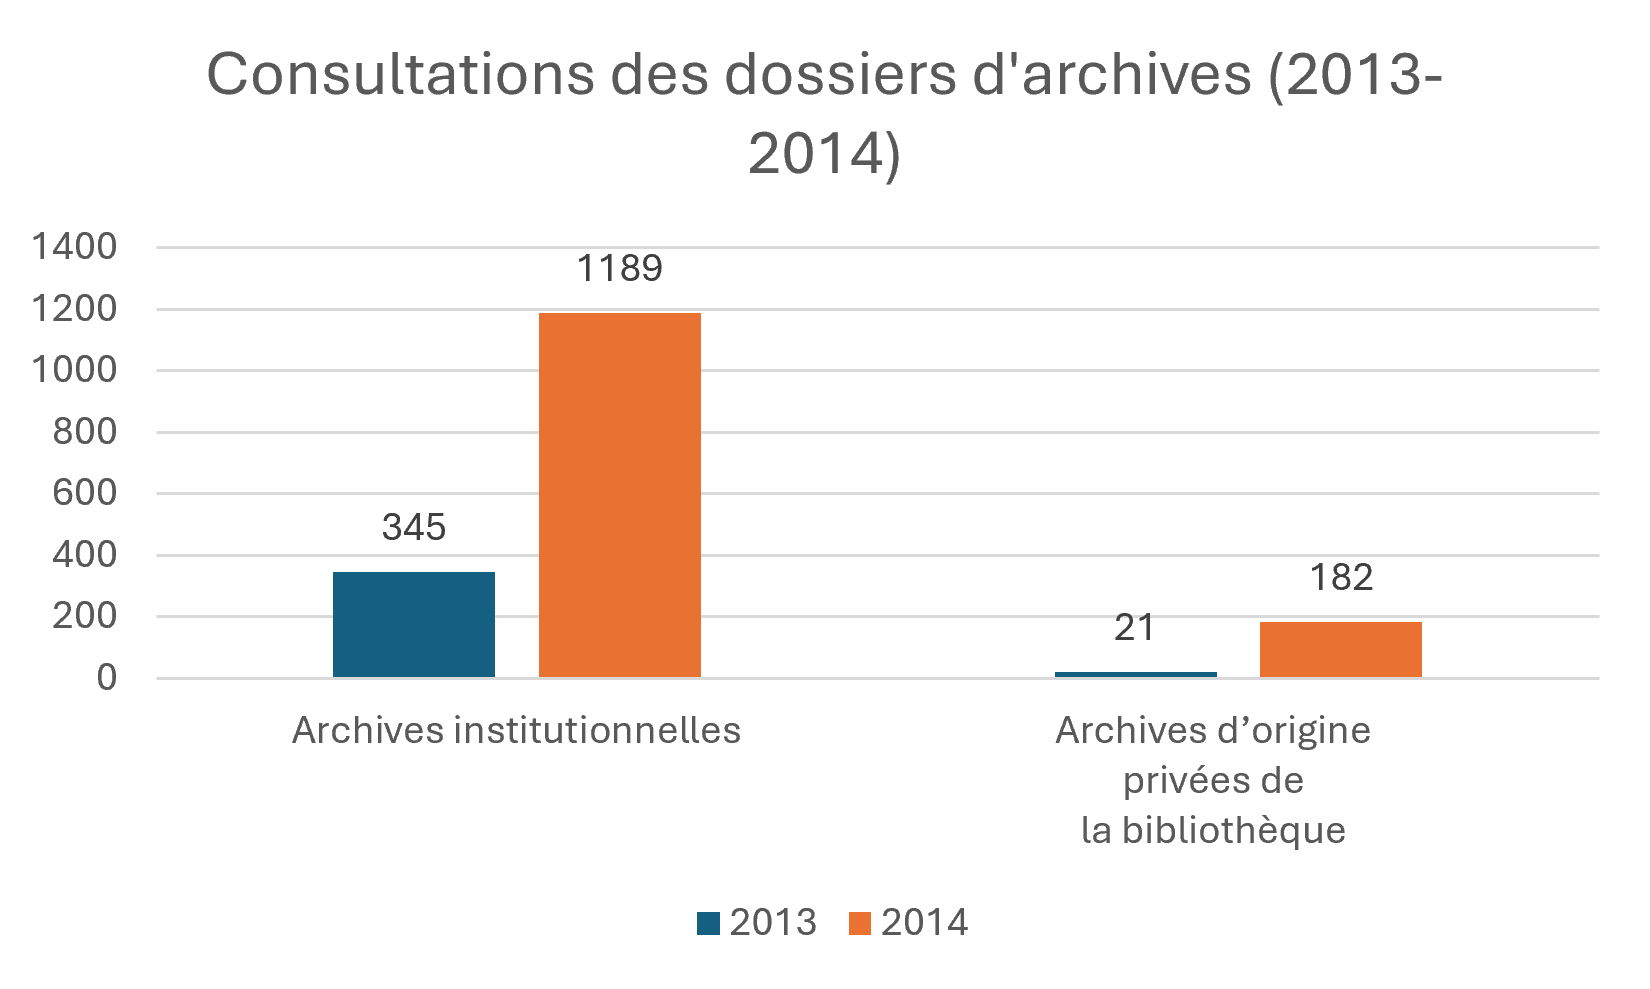
\includegraphics[width=0.8\textwidth]{Images/Consultation.png}
	\caption{Évolution du nombre de consultation des dossiers d'archives entre 2013 et 2014}
	\label{fig:Consultation}
\end{figure}

En 2013, 345 dossiers d’archives institutionnelles et 21 dossiers d’archives privées de la bibliothèque sont consultés, contre 1189 dossiers d’archives institutionnelles et 182 dossiers d’archives privées, en 2014. Cette forte augmentation représente plus de 270 ~\% du nombre de dossiers communiqués\footnote{Figure de statistique du nombre de consultation entre 2013-2014}. Le nombre total des lecteurs ayant consultés les archives en salle de lecture est également en hausse puisque sont dénombrés, 92 lecteurs en 2014 contre 85 en 2013.


\subsection*{La poursuite d’un renforcement de compétences}

Après les années 2018, principalement denses en matière de versement d’archives par les services de l’institution, l’année 2019 marque la transition, du fait du départ de l’archiviste. On note un versement important, de la direction de la Communication portant sur les dossiers de promotion des expositions et des activités des services de l’UCAD pour la période 1982-2017\footnote{Rapport d’activité 2014, p. 32, \cite{JP801-rapports}.}. Fin 2019, la directrice de la bibliothèque, Stéphanie Rivoire, propose de créer un service Archives dans l’optique de pallier les problèmes de traitement et de gestion documentaire. Karine Bomel est recrutée comme responsable du service Archives, puis Marie Dion la rejoint en 2020 en tant qu’archiviste chargée des archives institutionnelles. La poursuite des réflexions sur l’archivage leur est confiée, tant sur le plan de la gouvernance de l’information que sur la consolidation d’une politique d’archivage. C'est à cette même époque que les questions sur le numérique deviennent pressantes. Les archives ne sont plus uniquement le fruit d’une production analogique, le passage à un nouveau support et  l’avènement d’une nouvelle forme de production documentaire s’imposent aussi.


\section{Les archives au MAD}

Le MAD produit des documents d’activité et données répartis en deux catégories, d’une part, les archives publiques générées par les activités conventionnées avec l’État et d'autre part les archives privées produites par ses autres activités. Ces catégories sont toutes deux encadrées par les réglementations européenne et française. En droit commun français, c’est le livre II du Code du patrimoine qui est consacré aux archives.

Dans son article L211-1, les archives sont définies comme \enquote{ l'ensemble des documents, y compris les données, quels que soient leur date, leur lieu de conservation, leur forme et leur support, produits ou reçus par toute personne physique ou morale et par tout service ou organisme public ou privé dans l'exercice de leur activité}\footnote{Conformément à l'article L211-4, \cite{code-patrimoine-legislative} .}. Au-delà de leur définition, les archives ne peuvent pas être appréhendées en dehors de leur contexte de création. Cette notion évoque des réalités distinctes sur les producteurs et le cadre dans lequel les documents sont produits. Elle subdivise la notion en deux catégories différentes : archives privées et publiques. Cette distinction est particulièrement intéressante au musée des Arts décoratifs, dont les fonds résultent d’une part de son activité courante, et d’autre part de donation des archives des créateurs et des particuliers.


\subsection*{Les archives privées}

Comme leur nom l’indique, les archives privées représentent les documents qui ne relèvent pas de la production de l’activité d’un organisme public, mais qui résultent plutôt de celle d’une personne morale de droit privé, un particulier, une famille ou une collectivité. L’article 211-5 les définit ainsi : \enquote{Les archives privées sont l'ensemble des documents définis à l'article L. 211-1 qui n'entrent pas dans le champ d'application de l'article L. 211-4}\footnote{Conformément à l'article L211-5, \cite{code-patrimoine-legislative}}. À noter que les archives privées présentant un intérêt historique et patrimonial pour l’État peuvent rentrer dans les collections publiques d’archives\footnote{\cite{francearchives-archives-privees}}.

Dans le monde des musées, il ressort que \enquote{les archives privées acquises, données ou léguées à un musée deviennent une propriété publique}\footnote{\cite{archives-en-musees-vademecum}}. Une fois entrées dans les collections nationales, elles deviennent inaliénables, imprescriptibles et insaisissables. C’est le contexte dans lequel se situent celles du MAD.

Les archives privées témoignent de la raison d’être scientifique de l’institution. On retrouve dans son actif les documents liés à des maisons de couture, des créateurs, d’artistes dans le domaine de la mode, du design, de la publicité, du mobilier, mais aussi de l’orfèvrerie, des associations, et même des collectionneurs. Elles sont réparties en cinq grands ensembles thématiques : Design et Arts décoratifs; Mode; Jouets, Publicité et Arts graphiques; Manuscrits; ce qui représente 806 mètres linéaires en réserve, et environ 20 mètres linéaires de fonds en cours de traitement\footnote{\cite{dion-archives-privees-2026}}.

\subsection*{Les archives institutionnelles}

Le Code du patrimoine définit les archives publiques comme :\enquote{Les documents qui procèdent de l’activité, dans le cadre de leur mission de service public, de l’État, des collectivités territoriales, des établissements publics et des autres personnes morales de droit public ou des personnes de droit privé chargées d’une telle mission}\footnote{Conformément à l'article L211-4, \cite{code-patrimoine-legislative} .}. Investi d’une mission de service publique, le musée des Arts décoratifs produit des archives publiques dans le cadre de ses activités scientifiques et administratives. Elles sont le résultat d’un fonctionnement quotidien, de prise de décision et, de tenue d'expositions.

Pour comprendre la structuration des archives institutionnelles, il convient de constater qu’elles s’organisent en deux grands ensembles distincts. Nous avons d’une part les archives administratives. Concrètement, il s’agit de documents produits ou reçus par les services dans le cadre de leur gestion courante. Elles reflètent en quelque sorte la mémoire vive de l’institution. Généralement, on y trouve les documents relatifs aux ressources humaines, au conseil d’administration et autres instances décisionnelles, aux finances au mécénat, aux bâtiments, à la sécurité des personnes et des biens, ainsi qu’à la communication. 

D’autre part, une seconde catégorie est liée aux documents produits dans le cadre d’activités scientifiques comme les expositions. Ces dossiers naissent du cheminement du processus de préparation, de conception, de réalisation, d’exploitation, de maintenance et d’évaluation d’une exposition. Les dossiers rassemblent la documentation des producteurs internes (services concernés par les expositions) et externes (les partenaires, les prestataires extérieurs et les mécènes).

C'est à ce niveau que se situe notre angle de recherche. Comprendre que les dossiers d’exposition aujourd’hui ne sont plus essentiellement constitués de supports analogiques mais aussi de supports numériques, et grâce au basculement des nouvelles technologies. Ce changement de paradigme bouscule la méthode de travail traditionnelle au sein de l’établissement.



\chapter{Transformation numérique des pratiques documentaires }

Le numérique est devenu un élément incontournable dans les organisations et s’impose à tous les domaines d’activité. Son impact affecte directement les administrations et les usagers qui se voient dans l’obligation de s'adapter. Dans ce contexte de mutation, la sphère archivistique n’est pas en reste : elle est directement concernée par ces changements qui modifient les modes de production, de gestion, de conservation et de communication des documents.

Ces évolutions prennent la forme de divers outils numériques, et aboutissent à l’augmentation de la production documentaire et à la multiplication des espaces de stockage. Pour répondre aux enjeux de dématérialisation et de pérennité des données et des documents numériques sur le long terme, les services d’archives doivent adapter leurs pratiques professionnelles. Le musée des Arts décoratifs s’inscrit dans cette dynamique en s’interrogeant sur les modalités de gouvernance. Au cours de ce processus d'évolution, les équipes sont confrontées à des préoccupations quant à la capacité de gestion de leur patrimoine documentaire et des espaces de stockage.

\section{La gestion documentaire face à l’apparition du boom numérique}

L'arrivée massive des outils informatiques a profondément modifié les méthodes de travail : on passe d'une production sur papier à une production nativement numérique. Ce qui entraîne la multiplication des documents, accentuée par le phénomène de télétravail. les institutions se retrouvent obligées de mettre en place véritable gouvernance documentaire pour encadrer cette situation, 

\subsection*{Transformation des pratiques professionnelles}

La mutation numérique est à l’origine de nombreux bouleversements au sein de la société et de ses administrations. Qu’elles soient publiques ou privées, les administrations se voient affectées par ces changements. Ceux-ci touchent à la fois la manière de produire  l’information, les différents supports qui la comportent, les moyens mis en place pour la rendre accessible, et la façon dont elle est conservée et traitée. 

Avec la dématérialisation des procédures, le développement d’outils bureautiques et d’applications métiers et la création des espaces de travail collaboratifs, la gestion documentaire se voit de plus en plus axée sur le numérique. Elle a une incidence sur la nature du document support qui en découlent, ce qui représente un enjeu majeur.

Dans le contexte des institutions muséales, la préparation d’une exposition se concentrait sur la production par les services, de courriers, plans, photographies, documents scénographiques, etc. Une partie importante de ces activités repose sur des objets matériels. La rédaction du courrier, qui doit être imprimé, transmis, annoté et classé dans un dossier,  en est un exemple : la production est contrainte par la matérialité des objets.

Or, avec la dématérialisation des procédures, la même activité de préparation d’une exposition se fait en suivant le même cheminement de base, mais en se conformant au nouveau support à gérer. À terme, on peut avoir les documents sous divers formats. À la seule différence que la production documentaire numérique est plus importante que celle de l’activité basée sur l’objet matériel. Ceci est une des conséquences de la dématérialisation. Les documents numériques sont produits, créés, modifiés et, copiés plus rapidement, leur support de création restant.

\subsection*{Augmentation du flux informationnel}

Après l’apparition des premières archives électroniques dans les années 1960, l’année 1980 est marquée par l’essor de la micro-informatique qui entraîne une toute autre dimension dans la gestion documentaire\footnote{\cite{archives-en-musees-electroniques}. p. 4.}. Les documents ne sont plus simplement substitués sous la forme papier, ils sont désormais produits nativement en format numérique, un mouvement qui s’étend progressivement à l’ensemble des supports (texte, son, images, données, etc.)\footnote{\cite{archives-en-musees-electroniques}. p. 4.}. Cette modification des modes de fonctionnement quotidien permet un gain de temps mais s'accompagne de nouveaux enjeux, tant sur le plan de la multiplicité et la rapide obsolescence des supports, des formats, des outils\footnote{\cite{archives-en-musees-electroniques}. p. 4.}, ue sur le plan de la perte de l’information en l’absence de structuration pensée en amont de la création des documents jusqu’à leur conservation.

\textbf{La crise sanitaire comme élément d’accroissement de la production documentaire}

En France et comme partout ailleurs dans le monde, l’année 2020 marque la transition brutale vers le travail à distance et le développement de nouveaux outils collaboratifs. Dans le contexte public français, le printemps 2020 constitue un cas d’école en ce sens où le taux de télétravail dans la fonction publique d’État, jusqu’alors marginal, est passé de 6,4 ~\% à 51 ~\% en quelques semaines\footnote{\cite{dgafp-teletravail-2020}. p. 2.}, sous l’effet du décret n°2020-524 du 5 mai 2020 modifiant le cadre réglementaire du télétravail à la fonction publique française. Plus clairement, l’article 2 alinéa-1 du présent décret octroie pour la première fois la possibilité d’un recours ponctuel au télétravail ; à ce titre, l’agent peut désormais mobiliser un volume de jours flottants selon ses besoins\footnote{\cite{decret-2020-524}}.

Malheureusement, ce changement soudain ne s’accompagne pas toujours d’un encadrement de la production documentaire due à la continuité d’activité. Un retour d’expérience piloté par la Direction générale de l’administration et de la fonction publique, à partir de groupes de travail réunissant les laboratoires stratégiques interministériels, les services RH ministériels et les plateformes régionales d’appui interministériel à la gestion des ressources humaines, confirme que ce basculement s’est opéré sans préparation préalable des salariés ni des managers, dont la plupart n’avaient jamais été formés au travail à distance auparavant\footnote{\cite{dgafp-teletravail-2020}. p. 5.}.

Avec un environnement de plus en plus fragmenté, l’information est très peu centralisée dans les organisations. Les documents sont éparpillés au sein de multiples espaces de stockage, ce qui complexifie leur repérage et leur exploitation. Cette dislocation entraîne une perte importante de métadonnées, et représente un véritable frein organisationnel.

Dans cet élan technologique, l’information à traiter s’est doublée d’une croissance quantitative. D’après la deuxième enquête serdaLAB menée en mars 2012 auprès de 230 organisations publiques et privées, 62 ~\%  des répondants désignent le volume croissant d’informations comme le défi principal de la gouvernance documentaire. Par ailleurs, 40 ~\% d’entre eux identifient comme enjeux majeurs le volume des documents internes et des informations externes, la multiplication des sources d'information, l'éparpillement des services en charge de la politique documentaire, ainsi que la perte de temps liée à la recherche des informations\footnote{\cite{serdalab-gouvernance-2012}. p. 6.}. Ces observations concernent aussi bien les organisations classiques que patrimoniales.

Cette problématique est relatée par le \textit{Business Document Unity} en 2025. Selon le baromètre France Num, 56 ~\%  des TPE-PME qui utilisent la plateforme d’échange de documents en ligne, mais souvent sans stratégie\footnote{\cite{nexpubica-gestion-documentaire}}.

Cette enquête permet de constater que le problème de fragmentation de l’information ne résulte pas forcément de l’accroissement de nouveaux outils technologiques, mais plutôt de l’absence d’organisation permettant un encadrement du circuit de leur production, de leur conservation jusqu’à leur communication. C’est à ce niveau que la gestion documentaire prend tout son sens. Dans la mesure où elle permet d’organiser le flux informationnel afin de faciliter leur accès et d’assurer leur traçabilité.\\[0.1cm]

Aujourd’hui, avec la production massive de documents numériques, la gestion documentaire devient complexe. Face à l’avènement des producteurs de documents et face à la diversité des espaces de stockage, la gestion documentaire atteint ses limites. Lorsque les règles de production, de conservation, de validation, de diffusion et de destruction des documents ne sont pas définies, il est impossible d’organiser les documents. Il devient donc important de développer une stratégie globale.

C’est dans ce contexte que s’impose progressivement la gouvernance documentaire appliquée au numérique. Là où la stratégie globale vient affirmer son attention sur les documents et leur cycle de vie, la gouvernance documentaire, elle, définit les règles de gestion qui s’appliquent à l’ensemble des dossiers et documents d’une entité, quel que soit leur support et la durée de leur cycle de vie\footnote{\cite{archives-vaudoises-gouvernance-documentaire}}. Son objectif est de définir, auprès des organismes, une politique documentaire commune visant à mettre en avant les responsabilités entre différents acteurs, à harmoniser les pratiques de gestion de l’information et à garantir le respect réglementaire, organisationnel et patrimonial. On comprend donc que le but de cette stratégie n’est pas de remplacer la gestion documentaire, mais plutôt de lui donner une dimension stratégique, et non plus uniquement technique. La définition d’une politique au sein d’une organisation se traduit par un document stratégique et directeur (ou un corpus de documents) qui formalise et décrit un ensemble de principes fondateurs, de règles, de méthodes et de recommandations techniques. Pour le sujet qui nous intéresse, la politique fournit donc le cadre général d’organisation, d’intervention, de contrôle et donc de gouvernance des documents d’activité\footnote{\cite{arnaud-2012}. p. 154.}.


\subsection*{Enjeux de la gestion documentaire au MAD}

Le \textit{vade-mecum} édité en 2013 par le réseau professionnel Archives en musées à l’usage des personnels des musées, entend faire le point sur les aspects liés à la question de la gestion des documents numériques. Il montre montre que le principal défi de l’archivage électronique réside dans l’organisation et la structuration de l’information en amont, dans la gestion du cycle de vie des données et des documents, ainsi que dans la gestion intelligente des dossiers hybrides papier où électronique\footnote{\cite{archives-en-musees-electroniques}. p. 5.}.

Ce sujet à portée globale trouve écho au sein du MAD. Du fait de son statut, le MAD ne doit pas gérer que les archives administratives des services supports, il doit veiller à la bonne tenue des dossiers d’œuvres, des fonds photographiques, de la documentation liée aux expositions temporaires et permanentes, aux autres événements ponctuels de médiation et valorisation des collections. Face à l’avènement de l’hybridité des supports, le musée ne veut pas seulement adopter un nouvel outil, mais plutôt structurer sa mémoire institutionnelle numérique.\\[0.1cm]

Dans l’optique de répondre à ces enjeux, l’équipe du service Archives  s’engage depuis 2020, en collaboration avec le service informatique sur une réflexion visant à mettre en place une gouvernance globale de l’information. À ce titre, plusieurs actions sont mises en place, à savoir la sensibilisation des salariés au cycle de vie des données et à leur archivage, la diffusion des règles d’usage des nouveaux outils, préconisant notamment des règles de nommage, de stockage, de sauvegarde, de mise en place d’un plan de classement, et la rédaction de tableaux de gestion\footnote{\cite{archives-en-musees-electroniques}. p. 4.}. Le but est de suivre de près les habitudes numériques des salariés, en proposant des solutions et des conseils de gestion par service ou au cas par cas\footnote{\cite{archives-en-musees-electroniques}. p. 4.}. Dans cet élan d’envergure stratégique, les archives d’exposition sont au centre de l’attention, en ce sens qu’elles constituent une activité transversale et centrale dans la production électronique courante de l’institution.



\section{La transformation numérique, une initiative pour le MAD}

Au MAD, la transformation numérique représente une nécessite pour la préservation de la mémoire que représentent les expositions. Il faut dont entre en mesure de garantir leur mémoire et s'assurer de la traçabilité des activées qui émanent d'elles.

\subsection*{Présentation du contexte institutionnel}

Avec l’avènement du numérique et le développement de nouvelles technologies, de nombreux organismes s’engagent dans une transformation de leurs pratiques documentaires. Au MAD par  exemple,  ce changement se matérialise par une vision globale de gouvernance de l’information à travers la maîtrise de la production, de l’organisation et de la conservation des documents numériques.

En tant qu’association relevant de la loi du 1er juillet 1901, et reconnue d’utilité publique depuis 1882\footnote{\cite{bomel-dion-mad-y-vas-2022}. p. 1.}. Le MAD renouvelle en 2022 son contrat avec l’Etat par une Délégation de Service Public jusqu’en 2032\footnote{\cite{bomel-dion-mad-y-vas-2022}. p. 1.}.


\subsection*{Une initiative numérique}

Dans le cadre du programme \enquote{Action publique 2022}, lancé par le gouvernement français en 2017\footnote{\cite{ditp-action-publique-2018}}, l’État ambitionne une vaste campagne de modernisation à destination des administrations publiques et des opérateurs rattachés à celles-ci. Le MAD  en tant qu’institution rattachée au ministère de la Culture, est directement concerné par cette nouvelle mesure nationale.

C’est sur cette base que le service Archives, déjà en quête de restructuration et d’amélioration, se lance à son tour dans la mise en œuvre de solutions concrètes visant à répondre aux besoins spécifiques liés à l’archivage tels que des projets numériques.

Le MAD a candidaté en 2022 et 2023 à l’appel à projets du Dispositif Interministériel d’Accompagnement des Missions pour l’Archivage Numérique (DIAMAN) qui est piloté par le Service interministériel des Archives de France (SIAF). Ce dispositif est à destination des grands corps de l’État tels ainsi qu’aux ministères et à leurs opérateurs rattachés qui souhaitent bénéficier d’une prestation d’assistance à maîtrise d’ouvrage (AMO) dans le cadre de la mise en œuvre de leur politique d’archivage numérique\footnote{\cite{bomel-dion-mad-y-vas-2022}. p. 2.}. Citons en premier lieu la candidature \textit{\enquote{MAD y VaS}} de 2022, qui avait pour objectif une étude préalable à l’archivage des données et fichiers du MAD dans la solution logiciel Vitam accessible en Service (VaS). Ce dernier est un système d’archivage électronique mutualisé pour les archives intermédiaires envisagé par les équipe du MAD puisqu'il proposait à long terme une possibilité d'interconnexion avec l'ADAMANT (Plateforme d’archivage électronique des Archives Nationales)\footnote{\cite{bomel-dion-mad-y-vas-2022}. p. 1.}. La candidature du MAD a été retenue en 2023 pour une prestation en 2024 recentrée sur une étude préalable à l’archivage des dossiers d’expositions stockés sur Teams, appelée DIAMAN MAD. L’aspect technique de développement d’un connecteur avec VaS a finalement été abandonné en cours de prestation puisqu’il ne résolvait pas la problématique initiale de restitution des données et métadonnées. 


\section{ Limites de la transformation numérique au sein de  l’institution}

En dépit des actions engagées en faveur de la gouvernance informationnelle, la transformation numérique demeure confrontée à plusieurs limites qu’il convient d’étudier avec attention. Si l'institution nourrit la volonté de mise en place d’une vague significative de projets, force est de constater que leur déploiement s’inscrit davantage dans une logique suite progressive que dans une mise en œuvre immédiate. Au mieux, des documents préparatoires tels que la formulation d’appel à projets, la note de cadrage, ainsi que le ou les dossier(s) de candidature, permettent de fixer les lignes directrices de chaque projet, de la conception jusqu’à sa réalisation. Cela facilite la transition vers l’utilisation de nouveaux outils et, une évolution croissante des pratiques professionnelles. Cependant, à ce jour, la gouvernance de l’information au MAD ne fait toujours l’objet d’un document formel ni d’une politique institutionnelle. 


\subsection*{Appropriation des nouveaux outils}

L’une des premières barrières rencontrées par l’institution se trouve dans l’appropriation par les salariés, des outils collaboratifs de la suite Microsoft Office 365 (Teams, OneDrive, SharePoint) récemment déployés. Toutefois, avec l’avènement de la crise sanitaire en 2020, l’obligation de migration technique des données vers de nouveaux environnements devient inévitable\footcite[version 4, p.~3]{bomel-dion-note-cadrage}. Les salariés se retrouvent contraints de réagencer, souvent dans la hâte, leurs méthodes de production et de partage documentaire — les circonstances n’ayant pas rendu possible l’anticipation de la  structuration de l’information.


\subsection*{Résistances et difficultés organisationnelles }

Les différentes actions menées par le service Archives auprès des services témoignent d’une ambition de résorber l’hétérogénéité des pratiques documentaires au sein de l’institution. Les entretiens réalisés conjointement avec le service informatique permettent de déceler les difficultés liées aux outils, à l’absence de structuration d’ensemble de l’information qui a pour conséquence une absence de production documentaire normalisée qui se retrouve dupliquée et dispersée. À ces constats, s’ajoute la non maîtrise des espaces de stockage individuels mis à la disposition du personnel\footcite[version 4, p.~4]{bomel-dion-note-cadrage}. Ces échanges ont montré l’importance de mettre mise à jour de la cartographie des systèmes d’information et de stockage, et la nécessité d’un accompagnement et de formations aux collaborateurs\footcite[version 4, p.~4]{bomel-dion-note-cadrage}. 

Dans le but de surmonter ces problématiques, les archivistes s’engagent dans une campagne de sensibilisation et de formation des services producteurs d’archives électroniques. En ce sens, elle donne les clés de gestion et de compréhension du cadre légal de la production documentaire dans l'institution — par essence, chacun est responsable de ce qu'il produit dans le cadre de l'exercice de ses fonction dans l'institution.

Ce processus conduit à des recommandations relevant de l’usage de nouveaux outils, du nommage de fichiers, du stockage, de la sauvegarde, ainsi que de la mise en place de plan de classement.

Pour mémoire, le projet DIAMAN prouve que l'institution n'est pas resté au stade de l'idée, mais qu'elle a mis en place des mécanismes pour avance et véritablement se saisir des enjeux.


\subsection*{Conséquences documentaires }

Les difficultés organisationnelles ont une conséquence directe sur la manière dont l’information est conservée. La deuxième version de la note de cadrage rédigée par le service Archives, mentionne que les documents sont dispersés entre plusieurs espaces de stockage, que les serveurs sont saturés, et que les doublons se multiplient à cause du manque de normalisation de l’information\footcite[version 2.]{bomel-dion-note-cadrage}.  De plus, les auteurs évoquent même un\enquote{vrac d'informations papier et numérique}\footcite[version 4, p.~4]{bomel-dion-note-cadrage} rendant la recherche fastidieuse, entraînant des risques en matière de contentieux de la protection des données personnelles.

Cette absence de structuration de données ne se limite pas à un enjeu de repérage : elle expose également à un risque d’obsolescence technologique, en ce sens qu’aucun document numérique n’existe de façon autonome, du fait de sa liaison à trois éléments techniques à savoir : son format qui détermine la façon dont l’information est encodée ; son support qui détermine le stockage physique et enfin son environnement logiciel c’est-à-dire le système d’information capable de lire et d’interpréter ce format. Contrairement au document papier, dont la lecture est effective tant qu’il existe physiquement, le document numérique risque de devenir illisible même s’il est parfaitement conservé, simplement parce que les technologies nécessaires à sa lecture sont dépassées. C’est là que repose tout l’enjeu de la pérennisation numérique à long terme.

L’étendue de ces informations éparpillées peut être évaluée grâce aux premières estimations des archives électroniques intermédiaires conservées sur les serveurs locaux et partagés de l’institution : en 2022, elles font état de plus d’1,2 million de fichiers représentant 3,25 téraoctets\footnote{\cite{bomel-dion-mad-y-vas-2022}. p. 4.}. À ces constats s’ajoute un élément fondamental : au moment de la rédaction de ce projet de fin d’études, les Arts décoratifs ne disposent toujours pas de système d’archivage électronique. Le dossier de la première candidature du musée au dispositif DIAMAN mentionne que l’association ne dispose pas de devis pour l’adhésion à VaS, ni à fortiori de système d’archivage électroniques et précise que le projet n’est pas encore déployé\footnote{\cite{bomel-dion-mad-y-vas-2022}. p. 4.}. Si depuis, le MAD a reçu un devis VaS basé sur le chiffrage réalisé lors de la prestation DIAMAN de 2024, il explore tous les scénarios d’archivage envisageables\footnote{\cite{dion-choix-archivage-2026}.} et n’a pour l’heure rien acté. 

 
\chapter{Genèse et caractéristiques  du « vrac numérique » des dossiers d’expositions sur le serveur YODA}

Si l’avènement du numérique pour les organisations a une incidence sur l’information comme le présente le chapitre précédent, cette partie se concentre sur sa réalité concrète. Aujourd’hui, une organisation non structurée peut représenter un défis important pour les gestionnaires de l’information du fait qu'elle connaît une accumulation. Cette dernière représente d'ailleurs souvent un frein pour son identification. Perçue comme le maillon fort du fonctionnement d’une société, sa structuration reste primordiale pour l’histoire de celle-ci. Au MAD, l’information se situe dans les activités métiers de l’institution ; dont les expositions. Les documents produits dans le cadre de cette activité sont conservés dans plusieurs espaces de stockage, dont un que nous allons étudier : le serveur local YODA. L’utilisation du mot \enquote{genèse} ici implique de présenter la fonction initiale du serveur. Parallèlement, il est question de faire le point sur ses caractéristiques.

À partir de ces éléments, nous avons structuré le chapitre de la manière suivante : une première partie est consacrée à la compréhension et la constitution globale du serveur; une deuxième porte sur les facteurs qui sont à l’origine du vrac qui le constitue; une troisième nous permet de réaliser une micro étude synthétique sur la manifestation réelle de ce vrac. C'est une notion qui trouve du sens dans l'écosystème numérique et analogique. Michel Remize décrit le vrac numérique comme un \enquote{entassement croissant et pas toujours cohérent de documents sur les serveurs [...] qui touche les entreprises comme les administrations}\footnote{\cite{remize-2021}.}. 

\section{d’un espace de stockage à un enjeu archivistique}

Le serveur YODA s’inscrit dans l’environnement documentaire du MAD puisqu’il est utilisé par tous les services comme un lieu de stockage des documents numériques. Toutefois, la considération et la place du serveur dans l’activité quotidienne de l'institution ont évolués au fils du temps. Aujourd’hui, l’ensemble des travaux engagés par le service Archives permettent de porter un regard critique sur les données qui le constituent.

\subsection*{YODA comme un espace de stockage}

Comme nous l’avons mentionné plus haut, il est important de comprendre que le serveur est local, c’est-à-dire un espace de stockage accessible uniquement au sein de l’institution ; utilisé pour les données  produites dans le cadre ses activités. La note de cadrage relative à la mise en place d’une gouvernance de l’information et d’une politique d’archivage nous présente son organisation. Elle met en avant la subdivision du serveur en deux espaces distincts: YODA I, étant considéré comme le serveur local commun utilisé pour les  données partagées ; et YODA H, un espace de stockage comportant les données individuelles des salariés\footcite[version 4, p.~4]{bomel-dion-note-cadrage}. Cette partition rend avantageuse la vision des producteurs sur la considération de la gestion de l’information dans la mesure où, l’information est créée, enregistrée, partagée et conservée sur des espaces auxquels ils ont un accès. C’est l’un des avantages  de la double facette du serveur : à la fois espace de travail et espace de stockage, il permet d’avoir accès à des informations usuellement distinctes au même endroit.

Dans le cadre des expositions, cette configuration du serveur est importante en raison du nombre d’acteurs qui interviennent dans la mise en œuvre. La préparation d’une exposition fait intervenir plusieurs services dans le même temps impartit, chacun avec une production documentaire qui lui est propre en fonction des missions assignées. Disposer d’un espace collaboratif, pour faciliter les échanges rapides sur d’éventuelles modifications de la documentation liée à l’exposition, et de disposer d’un espace pour conserver les documents validés facilitent le travail entre les salariés.

Toutefois, avant de continuer sur ce point, il convient de s’attarder sur un point : a distinction existant entre un espace de stockage et un véritable archivage. Le dépôt d’un fichier sur un serveur répond  dans un premier temps aux besoins d’emplacement, de sauvegarde et éventuellement d’accessibilité. Cette action n’implique pas forcément un dépôt dans une arborescence structurée car rien n’oblige un classement préalable. Ce dépôt ne garantit pas non plus le devenir des documents. Il est donc nécessaire pour les administrations de mettre en place des moyens qui encadrent la conservation des documents présents dans un espace de stockage. Dans le cas du serveur YODA, il est important d’indiquer qu’il n’a pas été conçu pour assurer les missions d’un système d’archivage électronique.


\subsection*{Coexistence progressive de plusieurs espaces}

À partir de 2020, l’organisation documentaire du MAD connaît une transformation significative. Tout ceci se matérialise dans le contexte de la crise sanitaire qui impose le télétravail. Les salariés n’ont alors plus accès à leur documents de travail stockés sur le serveur local dédié appelé YODA. Il ne peut donc plus être un espace de travail à utilité courante. En avril 2020, c'est la solution Microsoft Office 365 qui est proposée et déployée par le service informatique qui est proposée et déployée par le service informatique afin de faciliter le travail des salariés  distance (connexion simple et rapide, plateforme collaborative, outil de visioconférence, de conversation, de partage, etc.)\footcite[version 4, p.~4]{bomel-dion-note-cadrage}. Pour accéder aux données et documents utiles pour la continuité des activités du MAD, la Direction Générale, met en place une séquence de migration. Elle se déroule en deux phases, tout d’abord pour migrer les données du serveur local commun YODA I vers Teams, puis les données de leur espace de stockage local YODA H vers l’espace de stockage individuel \textit{OneDrive}\footcite[version 4, p.~4]{bomel-dion-note-cadrage}. Cette mission répond à la limite du serveur local, perçu comme obsolète, saturé et difficilement accessible à distance.\\[0.1cm]

L’apparition de ces nouveaux outils ne résout pas à toutes les difficultés documentaires rencontrées avant la crise sanitaire (COVID-19), et en crée même de nouvelles.  C'est d'ailleurs important de souligner que c’est grâce à la transition vers le nouvel environnement collaboratif qui les défaillances préexistantes de la gestion documentaire sont révélées. Les modalités de structuration de l’information n’étant pas encadrées, il devient compliqué d’assurer, même avec de nouveaux outils de travail optimisés, une  gestion efficace de l’information. Cette situation nous amène à comprendre qu’avec la coexistence de plusieurs espaces de stockage et de travail, les données se retrouvent dispersées à plusieurs endroits. Cette dispersion de l’information aurait pu être anticipée et entérinée par la structuration mais les difficultés évoquées plus haut n’ont pas permis une telle transition et des solutions doivent maintenant être trouvées pour résoudre diverses problématiques inscrites dans la note de cadrage sur la gouvernance de l'information de 2025. Cette dernière soulève une problématique fondamentale, celle de l’accès à l’information. En effet, confronté à cette sphère informationnelle, plusieurs producteurs peine à retrouver leurs documents en raison de la masse d’information enregistrées dans les espaces. 


\subsection*{De l’espace de stockage à l’objet de traitement}

Au vue des difficultés rencontrées, il devient important de porter un regard sur les données du serveur. C’est dans cette même dynamique que le service Archives ne le considère plus comme un simple espace technique de stockage, mais comme un espace d’archives intermédiaires avec des données qu’il convient d’organiser, de structurer et de traiter avant le versement dans un système d’archivage électronique. Cette évolution se remarque dans le cas des dossiers d’exposition où; a production issue d’une multitude d’activités et de producteurs représente aujourd’hui une masse documentaire importante. Les documents dans les espaces de stockage doivent être facilement repérables, pour permettre, non seulement à l’institution de conserver sa mémoire patrimoniale, mais aussi pour  répondre aux exigence légales et réglementaires en matière de conservation\footcite[version 4, p.~7]{bomel-dion-note-cadrage}.

C’est là que notre analyse prend tout son sens. Au départ perçu comme un simple espace de stockage, on se rend compte qu’une fois les données créées celles-ci nécessitent une organisation qui concerne à la fois les archivistes, les producteurs et les usagers (personnes qui consultent les documents). Sans cette organisation, une structuration hétérogène apparaît, le vrac. Il est intéressant de noter que ce dernier n'est pas la résultante d’un fait mais de plusieurs facteurs.


\section{Facteurs de constitution croissante du vrac  numérique}

Dans la réflexion sur le caractère symptomatique du vrac que représente le serveur YODA, il convient de comprendre les facteurs qui sont à l’origine de cette anomalie fragilisant  le fonctionnement d’une institution. Notre étude permet de distinguer deux points essentiels, un au niveau de la nature de l’exposition et un autre au niveau manque de cohésion sur le plan de la gestion informationnelle.


\subsection*{La transversalité des expositions à l’épreuve d’une organisation en silos}

Dans les institutions muséales, le vrac numérique est lié dans un premier temps à un décalage structurel entre la nature des projets menés et l’organisation qui les accompagne. Une exposition ne se réalise généralement pas à partir des actions menées par une seule personne mais par  synergie de plusieurs corps de métiers et de plusieurs services.

Dans le contexte du MAD, elle résulte de la collaboration en interne entre la direction des musées et les autres directions : conservateurs, graphistes, scénographes, agents de sécurité, régisseurs, juristes, etc. Tous ces acteurs produisent des documents de nature différente mais liés à un seul objet : l’exposition. Pourtant, la structure documentaire actuelle du MAD — et celle du serveur YODA — se répartit en service, et non pas par exposition. Par conséquent, chaque service dispose d’une arborescence qui lui est propre, d’une partie de l’espace de stockage qui lui est attribué, d’une convention de nommage partagé au sein d’un groupe plus restreint que celui constitué pour faire vivre le projet. De surcroît, aucun dossier unique ne permet de compiler l’ensemble de la masse documentaire créée autour d’un projet d’exposition. Ces constats expliquent que le conflit existant entre le type d'organisation et la nature intrinsèquement transversale des dossiers d’exposition.


\subsection*{L’absence d’une gouvernance documentaire commune}

La sectorisation de la production documentaire par service ne constitue pas toujours un risque de création d’un vrac. La structuration documentaire réfléchie en amont des projets permet d’anticiper et de structurer l’ensemble. Dans le cas de notre étude, la gestion s’est faite sans encadrement et a conduit à la constitution d’une masse non identifiable. Les différents entretiens avec l’archiviste font remonter une problématique centrale pour nous : l’absence d’une gouvernance documentaire. Ce point constitue le second facteur de création du vrac numérique. Le fait que les  producteurs créent des documents qu’ils ne sont pas capables de retrouver constitue un signal d’alarme à la fois pour eux, mais aussi pour la direction.

En 2012, Natalia Bauer relève ce point d’une importance capitale dans un audit. Elle remarque l’urgence d’instaurer une gouvernance documentaire dans le but d’organiser la production documentaire et ainsi pour répondre aux défis de conservation de la mémoire de l’institution. Pour elle, l’absence d’uniformisation qui encadre la gestion documentaire est un enjeu qui affecte à la fois les espaces de stockage physiques mais aussi électroniques. 
Le nommage est l’un des aspects qui captive le plus dans un environnement de productivité documentaire\footnote{\cite{bauer-archives-publiques-2012}. p. 12.}. La coordination de nommage a pour but, entre autres, de faciliter le travail de l’archiviste dans ses missions de classement et traitement. En son absence, il devient difficile d’identifier le contenu des documents sans avoir à l'ouvrir. Le nommage permet également de classer plus rapidement les documents tant pour les producteurs que pour l’archiviste.


\section{Manifestation du vrac dans les dossiers d’exposition}

Après avoir répondu à la question : pourquoi le vrac numérique que nous étudions existe ? Il est important de savoir comment il se manifeste. Au préalable, il faut souligner que ce n'est pas parce qu’on est face à un volume important de données que celles-ci constituent un vrac. La quantité des données ne s’accompagne pas forcément d’un état de non structuration.

Plusieurs mécanismes permettent d’apporter une distinction et de caractériser ce qui constitue réellement un vrac. Marie Anne-Chabin, dans son article sur le vrac numérique, fait la nuance entre deux aspects du vrac. D’abord, elle introduit la notion de \enquote{vrac-désordre}, caractérisé par l'absence de règles de nommage et d’une impossibilité de connaître le contenu ou la valeur d'un document sans l'ouvrir. Ensuite, elle mentionne le vrac au sens de conditionnement, où les documents, bien que non individuellement classés, restent correctement qualifiés par leur provenance, leur statut ou leur valeur archivistique\footnote{\cite{chabin-vrac-2016}.}. Selon elle, ce n'est donc pas le volume en tant que tel qui définit le vrac mais l'absence de qualification et d'identification des documents qui le composent.


\subsection*{L’accumulation de l’information}

Lorsque nous nous trouvons confrontés à une ensemble documentaire, l’une des premières caractéristiques qui retient notre attention c’est le phénomène d’accumulation. Ce dernier caractérise généralement et en apparence la notion de vrac. Dans notre étude, elle permet de qualifier le serveur YODA.  À partir du processus de coopération entre les services dans le cadre de la réalisation d’une exposition, plusieurs documents sont produits (documents administratifs, scientifiques, photographies, documents relatifs aux prêts et à la régie des œuvres) et regroupés dans un seul et même espace. Le serveur YODA est par ailleurs aujourd’hui considéré comme un espace de stockage passif de la production ancienne puisqu’il conserve les dossiers d’exposition d’avant 2018\footcite[version 4, p.~4]{bomel-dion-note-cadrage}. Il s'agit d'un arriéré à traiter.

Cependant, il serait erroné de considérer automatiquement  cette accumulation comme une anomalie. Si on s’en tient au principe archivistique du respect des fonds, les documents produits, accumulés par un service au cours de l’exercice de ses activités reflètent et documentent cette activité. Le concept d’accumulation tel que présenté nous intéresse pour notre étude, car  il permet d’identifier les documents réunis ensemble et produits soit par une même personne, soit par un groupe. On peut penser que comme les services du MAD collaborent dans le cadre de l’activité muséale, il s'ensuit forcément une production commune. Il n’en est rien. Bien que l’objet soit commun, les services produisent des documents de façon indépendante, en silo. Les fichiers d’une même exposition se retrouvent donc répartis dans le serveur à plusieurs endroits et sans traitement.


\subsection*{Le phénomène de doublons}

Le second mécanisme qui caractérise le vrac du serveur YODA c’est la duplication des fichiers. Ce phénomène s’observe par la présence de fichiers identiques et plusieurs versions d’un même document. Ce mécanisme est la manifestation la plus parlante d’un travail collectif sans espace de stockage commun. C’est un phénomène courant, parce qu’un document peut être utile pour la documentation d’un service comme à un autre, chacun se retrouve avec une copie du même document. Au cours de notre développement, nous avons évoqué le phénomène de transversalité, dans la mesure où une même exposition peut regrouper des typologies documentaires variées : comptes rendus, plans scénographiques, documents liés aux contentieux, à la gestion des œuvres ou encore à leur communication. Ces documents émanent de l’activité des différents acteurs qui participent à sa réalisation. Chacun d’eux conserve dans son espace de stockage propre une partie des documents. Cette conservation différenciée et plurielle aboutit \textit{in fine} à la naissance à des doublons. Cette situation n’est pas favorable à la production croissante et structurée de documents. La considération que l’on a des doublons permet de faire la distinction entre doublon strict et fichiers identiques. Ce que nous pouvons dire à ce niveau, c'est que pour distinguer deux fichiers identiques, il est judicieux de calculer leur empreinte numérique (hash). 



% ----------- Partie II --------

\part{Fondements théoriques du traitement des archives numériques d’exposition}

\chapter{La diplomatique de l'archive d'exposition et son cycle de vie}

La situation de crise documentaire évoquée dans le chapitre précédent fait remonter plusieurs problématiques ayant une incidence sur la gestion documentaire, à l'instar de la perte de l'information. Dans un tel environnement, l'information ne se perd pas seulement à cause d'un mauvais rangement des fichiers. Cela est également lié à des réflexes quotidiens des salariés tels que la copie des fichiers des espaces de stockage individuels vers les espaces partagés, leur déplacement d'une arborescence à une autre,  réflexes souvent perçus sans risque au premier abord. Pour remédier à cette situation, Luciana Duranti présente dans son article sur \textit{\enquote{la diplomatique des documents électroniques}} que la diplomatique est la science fondamentale qui détermine les caractéristiques extrinsèques  et intrinsèques des documents. Son étude prend appui sur les documents numériques\footnote{\cite{duranti-2003}}.

L'analyse de ces propriétés exige de mettre l'accent sur le statut profond du document. Ce qui impose une analyse rigoureuse des caractéristiques intrinsèques des documents :  sa nature, son authenticité et son contexte de production. En effet, cette approche fondée sur trois composantes est ce qui donne du sens à la transformation d'un vrac numérique passif en un fonds exploitable et sécurisé. Elle se décline en plusieurs articulations : la première approche se concentre sur la typologie documentaire et la valeur administrative; la deuxième sur les conditions d'altération et la sur la valeur probante des documents; la troisième met en avant les liens organiques entre les documents et les activités qui les génèrent. 

Cette approche diplomatique trouve une limite d'application dans le contexte du MAD, du fait de plusieurs facteurs : l'absence de charte documentaire ou éditorial :  aucun document d'une même typologie ne se ressemble, ni ne possède la même structure interne.

Le présent chapitre s’appuie sur ce cadre théorique et se propose de faire une étude fine : sur la nature et les valeurs de l'archive d'exposition, son évolution au fil du temps, avant de se concentrer sur les moyens de restitution du contexte face à une désorganisation.


\section{Nature juridique et historique d’une archive d'exposition}

 \textit{\enquote{La problématique des archives des musées en France se révèle aujourd’hui particulièrement complexe à appréhender pour les professionnels du patrimoine}\footnote{\cite{sasseti-aguilera-2020}. p. 227.}}.
 \textit{Véronique Sassetti-Aguilera}
 
 
La place des archives au sein des musées est une question brûlante. Elles répondent aux besoins à la fois ponctuels et historiques des organisations. Pour les comprendre, il faut être en mesure de déterminer leur nature, leur valeur et la manière dont elles évoluent dans le temps.


\subsection*{Une archive composite et plurielle}

À la différence d'autres séries documentaires produites dans les musées telles que les dossiers du personnel, les dossiers des marchés où les procès verbaux du conseil d’administration; les archives d'exposition se distinguent par leur caractère transversal. Elles constituent la production cloisonnée et interactive d'un ensemble de producteurs. 

En effet, elles sont appréhendées comme une construction collective dont la cohérence ne repose pas sur l'unité de son producteur mais sur l'unité du projet d'exposition. Les archives d'exposition sont le fruit d'un ensemble complexe. Ce qui donne du sens à cet ensemble c'est l'activité productrice, le projet d'exposition. Cette perception permet de rallier les archives à tout ensemble de logiques. Elles s'inscrivent dans la logique :  administrative, en ce sens ou elle émane d'un projet; scientifique, car elles résultent d'une réflexion et d'échanges autour des œuvres muséale,  parce qu'elles sont le produit d'une activité de conception exposition ;  et communicationnelle, par les documents de la médiation et de diffusion des expositions.

\subsection*{La valeur de preuve et de mémoire}

Selon Théodore Schellenberg, les documents publics modernes disposent de deux types de valeurs : la valeur primaire (c'est celle qui est utile à l'organisme pour les besoins de preuve, notamment financières, juridiques, administratives ou opérationnels), et la valeur secondaire (utile à d'autres organismes ou au public une fois que le document n'est plus utilisé au quotidien)\footnote{\cite{schellenberg-appraisal-1956}. p. 6-7. }. L'auteur s'appuie sur l'utilité de façon durable des archives dans les institutions publiques pour mûrir sa réflexion. Dans la valeur secondaire, il identifie la valeur probante comme étant ce que prouve le document sur l'organisation, les fonctions et le fonctionnement de l'organisme qui l'a produit\footnote{\cite{schellenberg-appraisal-1956}. p. 6-7. }. En d'autres termes, l'archive remplit une fonction de preuve dans le cadre de l'activité ponctuelle d'un organisme à travers sa valeur primaire. Elle documente et témoigne de l'organisation, du fonctionnement et des actions de l’institution dans la durée, en vertu de sa valeur probante. Au-delà de cet aspect, l'archive est la mémoire de l'institution, puisqu'à travers ses documents, elle peut retracer sont histoire depuis la genèse.

Dans le contexte de l'exposition, l'archive prouve, une fois l'exposition terminée, comment le musée à fonctionné pour réaliser ce type de projets : elle retrace le processus institutionnel qui a permis de produire l'exposition (les décisions prises, les procédures, les acteurs et leurs responsabilités). Ces informations, portant sur des décennies, et qui concernent plusieurs expositions, constituent la mémoire organisationnelle et présentent un intérêt pour les agents, en premier lieu, et pour les chercheurs, dans un second temps. Cet intérêt en deux temps se recoupe avec les écrits de Schellenberg : les agents s’intéressent à la valeur primaire tandis que les chercheurs cultivent leur intérêt pour la valeur secondaire, la valeur probante. 

\section{Application du cycle de vie des documents au contexte numérique du MAD}

Le cycle de vie est appréhendé comme l'ensemble des étapes de l'existence d'un document de sa création à la mise œuvre de son sort final\footnote{\cite{kern-holgado-cottin-2015}.}. Dans la conception archivistique, Yves Pérotin fait une présentation de la \enquote{théorie des trois âges}, dans son article sur \textit{L'administration et les \enquote{trois âges} des Archives}. Selon lui, les trois moments de la vie d'un document sont : l'âge administratif, l'âge de pré-archivage et des dépôts intermédiaires, pour finir avec l'âge de l'archivage\footnote{\cite{perotin-administration-1961}}.

Le modèle cible envisagé par le MAD pour structurer ces trois âges, à travers les différents choix d'archivage numérique possible à chaque étape du cible de vie, est présenté en annexe\footnote{Voir annexe ~\ref{annexe:choix-archivage}}. 


\subsection{Création, utilisation et circulation du document}


Les documents sont produits par les agents qui se mobilisent autour d'une exposition, en particulier le service de la production des expositions, et les conservateurs. Dans le cas d'archives numériques, ceux-ci sont conservés sur deux ensembles de stockage : les stockages locaux (serveurx, Bureau, Mes documents, téléchargement, etc.) et dans le cloud Microsoft (Equipe Teams/SharePoint, OneDrive, ainsi qu'Outlook)\footnote{\cite{dion-choix-archivage-2026}. p. 1.}. Les documents sont manipulés, modifiés et échangés justifiant leur utilisation courante : ils circulent sous formes de pièces jointes ou lien de partage par échanges de mails. Les différentes versions détenues par les producteurs sont également partagées via les plateformes de collaboration. 

Cette phase de circulation active d'un document prend fin lorsque le document n'est plus utilisé pour le travail courant, généralement à la fin d'une exposition. Ce processus amorce le passage vers la phase intermédiaire.



\subsection*{Du document courant à l’archive intermédiaire}


Arrivé à la fin de son utilité quotidienne, le document n'est pas archivé automatiquement. Pour qu'il le soit, il faut qu'il passe par la phase intermédiaire. Au cours de cette dernière, il peut être consulté pour des besoins ponctuels ou administratifs, par l'archiviste et par les collaborateurs, et conservé pendant sa durée d'utilité administrative. Dans le cas d'espèce, le basculement de la phase courant à la phase intermédiaire se décline en plusieurs articulations : 

\begin{itemize}[label=---]
	\item \textbf{Cas1}: S'il n'a pas les droits, le service informatique donne accès à l'archiviste après traitement du producteur.
	\item \textbf{Cas2}: Le producteur effectue lui-même le versement manuel sur l'espace dédié.
	\item \textbf{Cas3}: Le service informatique effectue un transfert manuel via la sauvegarde, notamment en cas d'urgence ou de départ d'un salarié.
	\item \textbf{Cas4}: Le producteur donne l'accès à l'archiviste, qui effectue lui-même une synchronisation manuelle\footnote{\cite{dion-choix-archivage-2026}. p. 1.}.

\end{itemize}

Ces situations sont pour la plupart le résultat d'une activité manuelle, exécutée soit par les intervenants directs d'un projet, soit par les personnes extérieures (l'une importante pour le bon déroulement du processus d'archivage, et l'autre pour la gestion et le suivi des activités techniques informatiques). Un cinquième scénario est envisagé si le Système Archivage électronique implémenté au sein de l'institution : le versement avec connecteur ou API (\textit{Application Programming Interface}). Il s'agit d'un recours automatisé à partir duquel les documents sont transférés automatiquement des espaces de stockage du producteur vers l'espace de dépôt des versements. L'API est la passerelle qui permet à deux logiciels de dialoguer entre eux\footnote{\cite{orange-api-2025}.}.

Quatre solutions d'archivage intermédiaire sont identifiées : le stockage sur serveur sécurisé et sauvegardé (YODA), un pan intermédiaire mutualisé (VaS), un externalisé sous agrément du service interministériel des archives de France et un interne (VITAM). La première représente la situation actuelle du MAD.


\subsection*{Le sort finale }

Parler du sort final d'un document revient à expliquer les moyens mis en œuvre pour assurer sa conservation définitive. En d'autre termes, il s'agit des processus qui concourent à ce que l'information soit conservée dans des conditions optimales afin de garantir son accès dans le temps. L'institution française en charge de la conservation des archives définitives des institutions patrimoniales comme le MAD est : les Archives nationales. Le versement est prévu à \enquote{l’échéance de la durée d’utilité administrative (DUA)des documents. Dans le cas des archives d’exposition, la DUA est de 10 ans à compter de la clôture du dossier d’exposition l’exposition environ 1 an après le démontage}\footcite[version 2, p.~4]{bomel-dion-note-cadrage}. Pour des besoins de conformité et de sécurité, l'information est transférée, de l'organisme vers le logiciel VITAM des Archives nationales repose. Ce transfert se base sur le modèle de l'OAIS (\textit{Open Archival Information System}), notamment à travers la conception d'un SIP (\textit{Submission Information Package}) : c'est le paquet d'archivage à verser. Sa structure et toutes les informations relatives au versement sont décrites dans un manifeste conforme au standard d'échange des données pour l'archivage (SEDA). 

\section{ Le plan de classement comme instrument de validation intellectuelle}

En archivistique, il existe plusieurs outils pour comprendre et faciliter la recherche et l'accès à l'information dans les institutions. Le plan de classement est l'outil de gestion fondamental qui permet la mise en ordre physique et intellectuelle des documents. Il constitue la représentation intellectuelle de l'activité des producteurs et permet de restituer les relations qui leur donnent un sens. Placé dans l'environnement électronique, le plan de classement est soumis à des contraintes de structure tout en bénéficiant de fonctionnalités inexistantes dans les organisations papiers\footnote{\cite{collet2012}. p. 245.}. Si le classement, qu'il soit papier ou électronique se base dans les deux cas sur une structure organisée, la nature du support modifie néanmoins les pratiques de consultation. Dans le cas du papier par exemple, l'archiviste peut, par peut déplacer un dossier pour des besoins de consultation en remplaçant y un fantôme — une simple feuille pour indiquer l'absence du dossier. Dans l'environnement numérique, cette pratique n'a pas d'équivalence direct : le fichier original demeure à son emplacement, et c'est une copie qui est faite dans un environnement sécurisé pour la consultation sur place, sans jamais déplacer ni retirer le document d'origine

\subsection*{Le classement fonctionnel et le principe de provenance}

Comme nous l'avons mentionné ci-dessus, l’exposition est produite dans le cadre d’une grande collaboration interne ce qui génère un quantité importante de documents. Dans le contexte numérique, les documents produits diffèrent selon leur format et leur type : on se retrouve donc face à une hétérogénéité des documents. Or, en archivistique, la forme ou le support des document n'a pas d'importance, dès lors qu'ils sont produits ou reçus dans le cadre d'une même activité, d'un même projet, ils sont considérés comme liés à un même ensemble archivistique.\\[0.1cm]

Donc si les documents sont séparés de leur contexte initiale, il faut être en mesure de retrouver une structure qui répond à deux questions: pourquoi les documents sont produits ou reçus ? Et à qu'elle activité sont-ils rattachés? \\[0.2cm]

Dans certains cas, a structuration de l'organisme se substitue à un classement organique. Les dossiers seraient organisés par services qui les a produits (exemple : la direction \enquote{DDIP}, pour tout ce qui est produit par la Direction du développement international et de la production). Cependant, les services en raison des éventuelles réorganisations internes, des fusions de services ou de directions rendant complexe une telle mise en œuvre. 

Pour éviter cela et répondre aux questions posées plus tôt, le MAD, se résout à un classement par fonctions. Aude Collet souligne à cet égard que le plan de classement, en tant que système d'intellectuel d'organisation, structure hiérarchiquement et de façon logique les catégories descriptives conçues pour faciliter le classement et le repérage des documents\footnote{\cite{collet2012}. p. 245.}. Elle fait allusion au type de plan de classement par \enquote{activités}, car c'est lui qui facilite la compréhension du contexte de création/réception des documents au sein d'une organisation\footnote{\cite{collet2012}. p. 248.}. 

Le cadre de classement des dossiers d’exposition du MAD illustre cette logique : il est repartit en onze grandes rubriques (Propos/ Concept, Gestion des ressources, Gestion des œuvres, Mise en espace, Sécurité, Communication, Animations, Publication, Fréquentation, Bilan, Itinérance), chacune d'elle représente une activité constitutive d'une exposition\footnote{Voir annexe~\ref{annexe:referentiel-dossiers-exposition}}. 
c'est notamment la recommandation des normes et standards du records management\footnote{\cite{collet2012}. p. 248.}.

La logique d'une organisation structurée répond principalement au principe de provenance des documents. Il est compris comme le principe selon lequel chaque document doit être placé dans le fonds d'archives dont il provient et, dans ce fonds, à sa place d'origine\footnote{\cite{lodolini1995}. p. 203.}. \textit{L'Abrégé d'archivistique} dans la même lancée stipule que : \enquote{Les documents émanant d'un même producteur doivent être regroupés sans être mélangés à d'autre}\footnote{\cite{aaf-abrege-2020}. p. 137.}. Or dans la réalité du MAD, les documents relatifs à une même exposition sont aujourd'hui dispersés entre les différents services producteurs, sans regroupement systématique. Le service Archives s'attache actuellement à faire la collecte de ces documents auprès de chaque service, avec pour objectif de constituer un dossier d'exposition unique préalable aux versements d'archives définitives — ce qui nous amène, à cet égard à considérer le projet d'exposition plutôt que chaque service producteur pris isolément, comme l'unité de regroupement pertinent pour ce principe.

\subsection*{Le respect des relations entre documents, producteurs et activités}

Au-delà de sa considération d'outil d'aide au rangement, le plan de classement permet d'établir les liens entre les documents, leurs producteurs et l'activité génératrice. La compréhension de cette logique repose sur des rubriques distinctes. 

À travers la structure du plan de classement des dossiers d'exposition du MAD, on constate que l'arborescence représente les activités constitutives d'un projet d'exposition. Les documents produits ou reçus, s’insèrent dans l'une des thématiques, matérialisant le lien entre le document et l'activité. En outre, ce système permet de documenter les relations entre le document et le producteur : dans un contexte transversal où  le service de la production des expositions, la régie, les commissaires et les prestataires externes collaborent, le plan de classement centralise leurs apports au sein d'un même espace fonctionnel. Le référentiel reflète chaque étape de la collaboration, préserve l’historique de création d'un document, garantissant la compréhension du fonds.



\chapter{Les piliers scientifiques de la pérennisation numérique}

La gestion des documents numériques est un challenge auquel doit faire face toutes les institutions car, elle concerne à la fois la donnée (l'information) et le support qui la conserve. Les principaux défis sont :  conservation de  information soit conservée, son exploitabilité et son son intelligibilité dans le temps. Ces trois points caractérisent, entre autres, la pérennisation numérique. Pour se faire, il est important de mettre l'accent sur la préservation du support, de l'information qui l'entoure avant de retrouver ce que le fichier traduit grâce à l'analyse sémantique. C'est l'objectif du présent chapitre.


\section{Intégrité de la donnée et risques d'obsolescence logique}

Avant de s’intéresser au document numérique et aux conditions techniques qui permettent de le conserver et le rendre accessible, il est important de revenir sur un point : ce n'est pas parce qu'un document est stocké dans un serveur qu'il reste, pour autant, consultable dans le temps. La conservation matérielle ne dépend garantit pas son accessibilité future : celle-ci dépend de ensemble de composantes techniques (format, logiciel, environnement de lecture) — qui peuvent disparaître, changer ou devenir incompatibles avec l'environnement qui permet d'y accéder. 

\subsection*{La dépendance du document numérique à son environnement technique}

L'accès au contenu d'un document diffère selon qu'il soit sur support papier, ou numérique. Dans le premier cas, l'accès au contenu  s'effectue directement par le support. Dans le second cas, il convient de s’assurer de la  mise en œuvre moyens techniques et dispositifs afin de faciliter l'accès, la consultation et l'exploitation de l'information. L'environnement technique représente le principal moyen d'accès à l'information sur support numérique. 

Le \textit{vade-mecum} \textit{Les archives électroniques} du réseau Archives en musées, rappelle à ce titre que les archives numériques se caractérisent par l'information, le format et le support. Le terme d'information renvoie c'est le contenu que l'on souhaite partager\footnote{\cite{archives-en-musees-electroniques}. p. 8.}. Le format représente l'une des couches qui permettent de coder cette information et la rendre interprétable par un logiciel\footnote{\cite{archives-en-musees-electroniques}. p.8 .}. Or \enquote{les logiciels sont des outils qui évoluent : nouvelles versions non compatibles, abandon de certains formats.}\footnote{\cite{archives-en-musees-electroniques}. p. 8.}. Cette citation permet de soulever un fait déterminant : la relation de dépendance entre le support de l'information et le contexte technique de création d'un document. Le serveur, quant à lui, est l'espace de stockage des documents numériques, il facilite le maintien des données disponibles dans un environnement technique mais il n'y garantit pas l'accès ni la lisibilité dans un environnement futur.

Le \textit{vade-mecum} fait la distinction entre trois concepts : le stockage, la sauvegarde et l'archivage. Le stockage est identifié comme commun aux deux autres concepts. Il s’agit de la simple conservation les documents et des données enregistrés à un endroit précis sans autre action. Il pose également une question matérielle et technique : choix du format adéquat en fonction du lieu de conservation des supports \footnote{\cite{archives-en-musees-electroniques}. p. 9.}. L'archivage, lui, constitue la veille sur ledit format ainsi que son support de stockage\footnote{\cite{archives-en-musees-electroniques}. p. 9.}. En effet, l’archivage est l’ensemble des moyens mis en œuvre pour assurer l’intégrité, la pérennisation, l’authenticité, la traçabilité et la sécurité des données. Elle implique donc deux actions supplémentaires par rapport au stockage : une copie sur support d'archivage dédié (sauvegarde) et la garantie d'une lisibilité indépendamment des outils logiciels qui l'on créée\footnote{\cite{archives-en-musees-electroniques}. p. 9}. Nous pouvons matérialiser ces propos par le schéma suivant:

\begin{figure}[H]
	\centering
	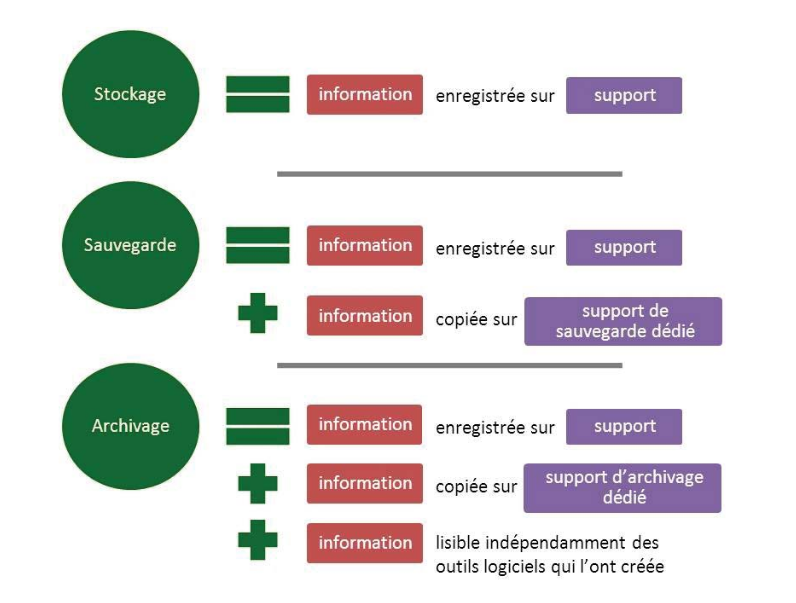
\includegraphics[width=0.8\textwidth]{Images/Archivage-et-Stockage.png}
	\caption{Distinction entre stockage, sauvegarde et archivage}
	\label{fig:Archivage-et-Stockage}
\end{figure}


Il faut avoir cette distinction en tête lorsque nous appréhendons les dossiers d'exposition stockés sur le serveur YODA. Ce dernier est un serveur de fichiers sécurisé qui fait l’objet de sauvegardes. Le fait que le serveur YODA constitue un espace de conservation intermédiaire ne signifie pas que tous les documents qui s'y trouvent sont seront lisibles et compréhensibles dans les années à venir. Cette observation renvoie à la nécessité de penser la conservation plus loin que le simple stockage du fichiers dans ledit  serveur. C’est dans ce cadre que l’archiviste a une expertise auprès du service informatique pour faire des préconisations sur la bonne gestion et conservation des documents et données. 

Cette instabilité explique pourquoi, tau MAD, la description des archives numériques se fait lors du versement à la préparation du SIP (paquet qui contient à la fois les fichiers, leurs métadonnées et un manifeste) parce que les métadonnées produites au moment de la création d'un document ne sont pas stables dans le temps. C'est le cas par exemple des documents stockés dans des serveurs partagés de type YODA. Ils peuvent être modifiés, déplacés, dupliqués, ce qui altère ce qui très souvent les métadonnées telles que la date de création, le chemin ou leurs liens avec d'autres versions auxquels ils sont liés. Ces actions créent le plus souvent des nouvelles métadonnées remplaçant les précédentes.

Cette réflexion rejoint la pensée de Luciana Duranti sur le document numérique. Elle considère que la diplomatique n'appréhende pas le document comme un contenu isolé, elle s’intéresse à la fois aux caractéristiques extrinsèques (le support, le format) et intrinsèques (contexte de création, le créateur, les actions, etc.)\footnote{\cite{duranti-2003}. p. 607.}. À partir de ces réflexions, il convent de s’interroger sur les risques liés à la conservation de ces documents.


\subsection*{Les risques liés à la conservation des documents}

Émilie Goubin identifie deux risques majeures liés à la gestion de l'information sur support numérique : \enquote{la conservation à long terme, risque lié à l'obsolescence des supports, des formats, mais aussi des organisations existantes; l'identification et la traçabilité, en lien avec [...] l'\enquote*{infobésité}et les risques juridiques}\footnote{\cite{goubin-2016}. p. 149.}. 

L'auteur aborde pas le risque lié à la conservation à long terme (l'obsolescence), d'un point de vue technique, et le subdivise en trois : 

\begin{itemize}[label=---]
	
\item{L'obsolescence des supports} : Il consiste en la fragilité physique des espaces de stockage des documents numériques, tels que les serveurs, les disques durs. 
\item{L'obsolescence des formats de fichiers} : Elle est causée par l'évolution des logiciels qui permettent de lire le format de fichier. C'est ce qui entraîne très souvent la perte de l'information\footnote{\cite{archives-en-musees-electroniques}. p. 8.}.
\item{L'obsolescence des organisations existantes} : Avec les fusions, la mutation des services, ainsi que la dématérialisation des procédures, une faille se crée au niveau de la fragilité du circuit habituel de l'information\footnote{\cite{goubin-2016}. p. 151.}. \\[0.1cm]

\end{itemize}

Le deuxième risque soulevé par Emilie Goubin, lié à la production de masse des données non structurées se caractérise par deux notions fondamentale : 

\begin{itemize}[label=---]
\item{L'infobésité} : C'est la surabondance d'information numérique présente quotidiennement et sous toutes ses formes\footnote{\cite{cigref2011risques}. p. 12.}.
\item{La perte de traçabilité}: Elle renvoie à la difficulté d'accéder au contexte de production d'une information, encore moins à son circuit dans une institution. 

\end{itemize}

Il est important de retenir que la conception archivistique, se doit de limiter les risques qui peuvent compromettre la lisibilité et l'intégrité d'un document numérique dans le temps.


\subsection*{Les principes de pérennisation}

Les besoins de pérennisation des documents après leur archivage soulèvent beaucoup de questionnements chez les archivistes, les conservateurs du patrimoine\footnote{\cite{chabin-2004}.}. Dans l'introduction de la revue consacrée au document numérique, Marie-Anne Chabin explique les raisons pour lesquelles la pérennisation est centrale aujourd'hui. Elle démontre que le nœud du problème se situe bien au de-là de la place du stockage, à ce titre, elle déclare que : \enquote{[...] c'est comment \enquote*{faire passer les années} à tous ces objets numériques [...] demain ou après-demain, pour pouvoir affirmer son droit, savoir ce qui s'est passé ou éviter de refaire ce qui a déjà été fait}\footnote{\cite{chabin-2004}.}. 

Pour garantir que les objets numérique ne perdent pas leur valeur de preuve, plusieurs moyens techniques et méthodologiques sont mobilisés. Le premier est le contrôle de l'intégrité qui permet de vérifier la cohérence de la de l'information. Le but est de vérifier que le document n'a subit aucune transformation, modification ou altération. Pour procéder à cette vérification, on peut utiliser l'empreinte numérique. La Bibliothèque nationale de France BnF la définit comme \enquote{une chaîne de caractères produite par l'analyse de données binaires (suite de 0 et de 1)}\footnote{\cite{bnf_integrite_donnees_numeriques}.}. Elle prend la forme d'un fichier ou un répertoire. Le but est de comparer les deux états d'un même objet numérique à des moments différents afin de vérifier s'il a été altéré\footnote{\cite{bnf_integrite_donnees_numeriques}.}.

Dans notre contexte de travail, cette empreinte n'est cependant pas exploitée pour des besoins de contrôle d'intégrité dans un premier temps, mais plutôt pour l'identification des doublons au sein du vrac numérique. \\[0.1cm]

Les deux autres points de la pérennisation sont le choix des formats et la migration. Pour s'assurer que les documents seront accessibles dans le temps, la décision du choix du format est importante, c'est se donner la possibilité d'accéder au contenu des fichiers dans le long terme. C'est une décision qui est propre à la volonté de chaque organisme en matière de conservation. À ce titre, en s'appuyant sur les recommandations imposée par le Référentiel général d'interopérabilité (RGI) aux administrations publiques, le MAD\footnote{\cite{bomel-dion-note-cadrage}. p. 4.} opte pour la répartition suivante : d'abord pour la bureautique, notamment, le PDF (\textit{Portable Document Format} / Archive), \textit{OPENDOCUMENT} et le TXT, ensuite pour les images telles que le PNG ou le TIFF, et éventuellement JPEG avec le moins de compression possible, et enfin pour les fichiers vidéos ou sonores les formats MPEG2, MPEG-4.\\[0.1cm]
		

Une fois le choix du format effectué, il convient de migrer les données du format actuel vers le format souhaité. Le fichier conserve ses fonctionnalités techniques de départ. La migration est appréhendée comme le passage d'un document d'un format non pérenne vers un format optimal. En d'autres termes, c'est le \enquote{transfert des données entre différents formats de données}\footnote{\cite{docuteam_formats_archivage}.}. 



\section{Métadonnées de structure et de préservation}

La conservation des documents numériques, telle que nous l’appréhendons dans cette partie se relève d’une forte une nécessité. Malgré les avantages qu'offrent les espaces de stockage informatiques, la problématique centrale de la pérennisation des informations demeure fondamentale. Après avoir abordé les opérations qui favorisent et permettent de rendre le document exploitable sur une longue période, on se demande maintenant : quelles sont les informations qu'on récupère pour atteindre l'objectif d'archivage?

Comme l’explique Émilie Goubin dans son article sur l'archivage électronique, l'archiviste, dans le contexte de l'identification des documents : \enquote{amené à identifier l'usage [...], l'identification de la mission pour laquelle un document est créé, [...]  l'usage qui peut être fait d'un document}\footnote{\cite{guyon-2023}. p. 152.}. Émilie Goubin va plus loin dans sa réflexion en mentionnant que l'identification du contexte de production d'un document numérique est un impératif pour la pérennité d'une archive.\footnote{\cite{guyon-2023}. p. 152.}. 

\subsection*{Identifier et décrire le document numérique}

Au-delà du nommage, chaque document dispose de propriétés techniques invisibles au premier abord, à l'instar de sa taille, son format, de sa date de création, ainsi que de ses dates de modifications. Ces métadonnées permettent de dresser la carte d'identité du document. En milieu patrimonial, d'après la Bibliothèque nationale de France (BnF), le document numérique est décrit par un identifiant unique et par un ensemble de métadonnées quelle subdivise en  trois grandes catégories \footnote{\cite{bnf-document-numerique-metadonnees}.}:


\textbf{Les métadonnées descriptives} : Il s'agit d'informations qui permettent de faire correspondre un document tant à son original ou qu'à ses différentes versions\footnote{\cite{bnf-document-numerique-metadonnees}}. Elles jouent le rôle d'identificateurs du document, puisqu’elles permettent d'identifier le son titre, son auteur, sa date de création et lien entre le documents et ses différentes versions.

\textbf{Les métadonnées de structure} : La BnF mentionne qu'il s'agit de, \enquote{rattacher les fichiers d'un même document entre eux, de restituer la structure du document: de connaître tous les fichier qui composent un document [...]; connaître la relation physique entre ces fichiers}\footnote{\cite{bnf-document-numerique-metadonnees}}.

\textbf{Les métadonnées administratives} : Elles garantissent la gouvernance constante de l'information. Elles répertorient les droits d'accès, notamment les droits d'auteur. Ces derniers comprennent les droits de confidentialité et les droits d'usage à savoir, la reproduction et la modification\footnote{\cite{bnf-document-numerique-metadonnees}}.
	
Cette classification n'est pas une simple théorie, elle correspond à des sections identifiées dans un format d'encodage réel et largement utilisé dans les institutions patrimoniales. Le standard METS (\textit{Metadata Encoding Transmission Standard}) utilisé pour décrire un document numérique à partir des métadonnées précise sur lui, il favorise son échange, sa gestion et sa préservation\footnote{\cite{bnf_mets}.}. Il se décompose en plusieurs sections dont; celle relative aux métadonnées descriptives (\texttt{descriptive metadata section/dmdSec} ), aux métadonnées administratives (\textit{administrative metadata section/amdSec}), et celle relative à la carte structurelle (\textit{structural map/StructMap}) , elle permet d'organiser la structure logique du document à partir de la liste des fichiers identifiés au niveau de section\texttt{file section/filSec} \footnote{\cite{bnf-document-numerique-metadonnees}}.\\[0.1cm]

Dans notre cas, contrairement à un document numérique constitué selon le standard METS, le vrac numérique se présente sous la forme d'une arborescence dépourvue d'encodage explicite. Pour étudier, on peut tout de même identifier la structural map comme l'arborescence ou la profondeur des dossiers (à titre d'exemple : \texttt{/Gestion-des-oeuvres/\allowbreak Pret/\allowbreak Dossier-Preteur/\allowbreak Fiche-de-pret.pdf}) en nous appuyant sur les outils d'archivistiques que nous évoquons à la troisième partie. Grâce à eux, on retrouve soit des métadonnées descriptives, des métadonnées administratives ou des métadonnées techniques.



\subsection*{Préserver le contexte et les relations documentaires}

Comme les autres types de documents, le document d'exposition ne constitue pas un objet isolé. Il est rattaché à un contexte précis, ici, l'exposition représente son principal contexte. À celui-ci, s'ajoute les différentes activités auxquelles il est lié, telles que la scénographie, la gestion des œuvres ou même la communication. Le document est aussi lié à la personne qui l'a produit ou reçu. Ces différentes appréhensions permettent de situer le document dans la chaîne documentaire à laquelle il appartient. La conservation des liens documentaires à aussi une grande importante dans le monde du numérique, car, comme nous l'avons mentionné dans les passages précédents, les documents se retrouvent dispersés dans plusieurs espaces de stockage. Face à cette dispersion, il est primordial de reconstituer la chaîne documentaire dont le document représente la trace. Les métadonnées constituent donc le moyens de faire remonter ces relation, en ce sens ou elles permettent d'identifier, le nom de l'auteur du document, à l'activité, ainsi que les différentes modifications effectuées sur le document.

Tout ceci nous amène à rapprocher la considération conception archivistique du document composante d'un fonds. Ses métadonnées retracent l'environnement documentaire auquel il est rattaché et mettent en évidence les liens entres les documents de cet ensemble, les opérations autours d'eux (modification, etc.).

\section{L'analyse sémantique au service de l'archivage}

Dans la pratique, l’archivage est complexe. Il convient de gérer l'information et les documents.  Cette gestion s’opère en tenant compte d’enjeux importants comme le traitement d'un ensemble éparpillé — problème fréquemment rencontré par les professionnels de l'information. L'identification de ces documents ne permet pas, à elle seule, de les gérer et d'assurer leur classement dans le fonds ou l'activité à laquelle ils sont liés. 

On se retrouve ainsi confronté à deux situations. D'abord les documents ayant les caractéristiques techniques similaires se retrouvent liés à plusieurs activités différentes. Ensuite, les documents d'une même activité ont des caractéristiques techniques similaires. 

Le classement d'un vrac va plus loin que le simple rangement des documents dans une arborescence fichiers ou alors dans un système d'archivage électronique. Face à la situation dans laquelle nous faisons face, nous nous posons la question de savoir :que représente réellement un document dans un dossier d'exposition? 
On constate qu'il implique la restitution de la fonction documentaire d'un document, ainsi que son rôle au sein d'une exposition. L'analyse sémantique apporte des éléments de réponse. 


\subsection*{Les limites d’un traitement fondé sur les caractéristiques techniques}

L'identification des caractéristiques techniques d'un document nécessite la mise en valeur des éléments tels que le format. L'écart entre la restitution du format et celui de la restitution de la fonction documentaire est considérable. Là où le premier ne fait référence qu'à l'aspect technique du document, l'autre s’intéresse à la place du document dans un ensemble. On se rend par exemple compte qu'une extension d'un fichier \enquote{.pdf}  peut renvoyer à  plusieurs catégories documentaires différentes en fonction de son contexte de création. Par exemple, un fichier .pdf qui peut très bien être un document lié au prêt des œuvres; un autre qui peut être centré sur la sécurité. Cette limite représente un enjeu pour la compréhension et la constitution d'un dossier d'exposition tel qu'il est perçu. Quelques outils d'aide au traitement archivistiques, prévus par les Archives nationales du Royaume-Uni confirment notre propos tel que l'outil qui permet de détecter les métadonnées techniques des documents\footnote{\cite{national-archives-droid}}. 



\subsection*{Le langage métier comme source d’information}

Le langage métier des producteurs constitue un élément primordial dans la reconstitution du contexte d'un document. Il favorise le traitement automatisé des documents. 

Au MAD comme la plupart des institutions, les salariés, dans l'optique de faciliter le repérage de leurs dossiers les identifient en fonction de leur vocabulaire professionnel, leur jargon. Ce vocabulaire très souvent lié à l'activité maîtresse à laquelle il est lié. Il est important en ce sens ou il permet \enquote{oui}, d'identifier l'activité, il n'est pas lié au vocabulaire informatique. 
Pour aller plus loin, il convient de préciser qu'un même sujet peut être abordé via un vocabulaire différent en fonction du métier, de ce fait on se retrouve avec un groupe de mots renvoyant à la même fonction, même utilisation ou même tâche sans que cela ne soit explicitement compréhensible. L'absence d'un thésaurus commun complique le travail de traitement archivistique et entraîne une multiplication des fichiers, voire l'apparition de doublons renommés pour faciliter la compréhension d'un corps de métier spécifique.


\chapter{L’automatisation au service du traitement archivistique}

Avec l'évolution progressive constante du métier d'archiviste et l’intégration poussée du numérique, une nouvelle approche se joue à la pratique archivistique : l'automatisation. Siham Alaoui s'interroge sur la place qu'occupe l'automatisation dans la chaîne de traitement archivistique\footnote{\cite{alaoui2024automatisation}. p. 20.}. L'auteure appuie sa réflexion sur la continuité de celle de Cook, qui lui identifie quatre paradigmes archivistiques, à savoir la preuve, la mémoire, l'identité et la communauté\footnote{\cite{alaoui2024automatisation}. p. 19-20.}. 

Face à cette évolution, l’automatisation se propose d'apporter des éléments de réponses techniques au traitement des archives numériques. En s’interrogeant sur le processus de traitement archivistique, elle vient en appuie au domaine. Avec la multiplication des supports, la quantité importante des données qui se retrouvent parfois dispersées, comme c'est le cas des données en vrac. Il devient alors difficile de repérer les informations, de les exploiter et de les mettre à la disposition des usagers. L'enjeu de ce chapitre est de s'interroger et d'identifier quels niveaux de la chaîne peuvent être automatisées tout en préservant les principes archivistiques afin d’alléger la tâche de l'archiviste.  On s’attellera à mettre en lumière l'utilisation de l'automatisation comme un levier d'amélioration et de fluidification des  traitements archivistiques. Parallèlement, on exposera les limites de ce système.

\section{Le changement d’échelle de traitement impliquant les archives numérique}

Les méthodes archivistiques restent valables dans l’environnement numérique mais leur mise en œuvre se confronte à une quantité de documents qui rend certaines opérations manuelles difficiles et chronophages. Dans le corpus étudié, on se rend compte qu'une même exposition peut se retrouver dans plusieurs répertoires, ce qui multiplie l'information.

\subsection*{Limites du traitement exclusivement manuel}

Le traitement manuel des archives est reste une opération contrôlée par l'archiviste. Il permet à l'archiviste d'être sûre de la véracité des informations recueillies et de la façon dont elles sont rangées. Toutefois ce traitement peut avoir des limites surtout face à la multiplication des supports et des données. 

Avec la masse importante de documents, le traitement des documents numériques représente une tâche fastidieuse. Plusieurs autres limites peuvent être soulevées. Sans nommage signifiant des fichiers, la gestion manuelle oblige l'ouverture individuelle et systématique des documents afin d'en identifier le contenu\footnote{\cite{chabin-vrac-2016}}. Il est à noter que cette opération peut être retardée par l'existence de conditions d'accès restrictives.


\subsection*{L’automatisation comme assistance au traitement de masse}

\begin{displayquote}
	\textit{\enquote{L'automatisation ne remplace pas l'intervention humaine\footnote{\cite{da-silva-santos-heiniger-2024}. p. 8.}}}.
\end{displayquote}
C'est ce que soulignent Sara Da Silva Santos et Fleur Heiniger. Face aux limites évoquées, l’automatisation ne se veut pas comme un outil de remplacement du traitement manuel, mais plutôt comme une aide. Celle-ci présente un réel avantage pour les archives numériques. Santos et Heiniger poursuivent en disant qu'elle\enquote{assiste la·le spécialiste dans l’identification des premiers problèmes qui créent du bruit autour des données : doublons, formats obsolètes, fichiers corrompus ou vides, etc.}\footnote{\cite{da-silva-santos-heiniger-2024}. p. 7.}. Ainsi, l'automatisation permet de réduire les délais d’exécution\footnote{\cite{da-silva-santos-heiniger-2024}. p. 6.} des tâches complexes en traitant un volume important et parfois non structurés. Un algorithme peut à la fois parcourir un ou plusieurs répertoires de fichiers, dans un temps très court, accélérant ainsi considérablement le traitement manuel qui prendrait des heures voir des jours à réaliser. Elle va plus loin en identifiant les données indésirables dans un grand ensemble, en effectuant le tri. Alaoui mentionne que l'automatisation représente une évolution du rôle de l'archiviste\footnote{\cite{alaoui2024automatisation}. p. 19-29.} en tant qu'acteur principal dans le processus. Il se retrouve dans un changement d'échelle auquel il doit s'adapter pour garantir le traitement des  documents. Cette adaptation relève d'un enjeu important étant donné que grâce à la maîtrise d'outils informatiques l'archiviste peut aujourd'hui exécuter ces tâches avec un plus de gain de temps.

Le programme présente une utilité lorsqu'il est conçu pour exécuter les tâches préalablement définies par l'humain. Ce dernier réunit un ensemble de conditions lui permettant de répondre aux exigences et à la demande du métier. Pour les archivistes, ces exigences soit à un besoin de tri, soit de classement, soit de structuration de la donnée. 



\section{De la règle archivistique à son interprétation informatique}

L'informatique est considérée aujourd'hui comme un étant un plus pour tous les domaines d'application. Les archives ne sont pas en reste. L’automatisation appliquée aux archives se subdivise en deux volets. D'un côté, le raisonnement archivistique : c'est l'idée maîtresse qui favorise la gestion documentaire. De l'autre côté, l'algorithme, qui joue le rôle de facilitateur, met en exécution de façon matérielle les règles qui sont indiquées en amont.

Dans la mesure où le programme ne sait pas en avance ce qui doit être exécuté, il ne peut pas imaginer les actions que l'humain veut mettre en œuvre. Ces règles ont besoin d’être formalisées. Cette formalisation réunit les deux notions évoquées plus haut.


\subsection*{Formaliser afin de rendre une décision automatisable}

Parler de formalisation revient à identifier l'ensemble des éléments qui permettent au programme d’exécuter des tâches et  faciliter la prise de décision\footnote{\cite{da-silva-santos-heiniger-2024}. p. 5.}. Dans le contexte archivistique,  elle nécessite d'identifier les phases qui permettent de repérer le traitement documentaire afin d’exécuter l'action à laquelle elles sont liées. C'est à cette étape que de l'archiviste se doit d'être pointilleux sur les recommandations faites. 

Comme nous l'avons mentionné plus haut, les simples caractéristiques techniques d'un fichier ne peuvent pas le décrire et le situer dans une arborescence.Il convient donc d'identifier la fonction documentaire sur la base d'autres éléments comme le nommage du fichier ou du répertoire auquel il est rattaché.C'est exactement à ce niveau qu'on peut comprendre ladite fonction.

La formalisation constitue une suite de conditions qui facilitent la mise en œuvre de ces indices. Elle permet de matérialiser différentes critères de sélection liés directement aux documents, à l'activité de laquelle ils découlent (si un document est produit ou reçu dans le cadre d'une activité de prêt par exemple), en lien avec le plan de classement. Cela ne traduit pas nécessairement le raisonnement archivistique en langage informatique, mais témoigne plutôt d'une collaboration étroite entre les deux. Il faut savoir que les règles simples et explicites favorisent la formalisation et, permettent l'exécution rapide des tâches.


\subsection*{La reproductibilité et la traçabilité des traitements}

La règle permet de rendre le traitement reproductible, de l'appliquer à un ensemble documentaire conséquent et de faire des tests appliqués à un corpus réel. Dans le traitement de masse, la reproductibilité représente un enjeu important, dans la mesure où elle permet la vérification et la comparaison des résultats d'un ou de plusieurs traitements. Sur la base de ces résultats, les professionnels disposent de la capacité de poursuivre, d'apporter des modifications ou alors de changer les règles identifiées plus haut.

Comme son nom l'indique, la traçabilité constitue l'action d'identification des opérations menées sur le corpus. Elle identifie les erreurs, les fichiers traités. Cette traçabilité peut se matérialiser lors du traitement par la génération des fichiers de logs, qui permettent de documenter chaque action algorithmique exercée sur un corpus. À partir de là, les réponses aux questions suivantes deviennent évidentes : \enquote{qui} (la personne qui a exécuté l'algorithme), \enquote{quoi} (l'objet sur lequel le traitement a lieu), \enquote{quand} (enregistre les différents moments de l'exécution), \enquote{comment} (la règle appliquée au corpus).



\section{ Les limites de l’automatisation et le maintien de l’expertise archivistique}

L'automatisation représente le moyen de faciliter le traitement de masse à grande échelle. Elle permet de standardiser les opérations archivistiques sérielles comme le tri, dont l'exécution exclusivement manuellement peut devenir difficile. Elle se heurte cependant à des limites qui rendent difficile son exécution, notamment au niveau de la prise de décision.

\subsection*{L’incertitude et les limites de la décisions}

Au regard de ce qui précède, nous pouvons dire que le programme informatique est aveugle au sens et au contexte. Là où l'outil informatique identifie les caractéristiques techniques des documents, l'humain lui interprète leur signification. Il convient de comprendre que le programme ne peut pas comprendre le contexte historique de son corpus. Les règles qu'il applique peuvent dans certains cas être incomplète de la réalité documentaire. Le programme exécute uniquement les instructions qui lui sont données. À partir de là, nous pouvons observer les limites décisionnelles que cela représente pour le traitement. Rien ne peut venir du programme informatique seul. Il ne peut pas décider les caractéristiques archivistiques à prendre en compte pour répondre aux exigences de conformité imposées par le métier.

C'est le cas dans le contexte du traitement des archives d'exposition, l'algorithme ne peut pas décider du vocabulaire qui doit être utilisé.



\subsection*{Une complémentarité entre traitement automatisé et validation humaine}

En réalité, avoir recours à l'automatisation c'est être capable de faire converger son savoir avec la compréhension informatique qui tourne derrière une machine. C'est à ce niveau qu'on remarque le travail collaboratif entre l'humain et la machine, où le traitement n’est pas purement informatique mais basé sur une vraie réflexion humaine. 
L'étude menée par Sara Da Silva Santos et Fleur Heiniger explique cette distinction. Selon leur développement, c'est l'humain qui définit en amont les règles et les lignes directives qui permettent au programme de fonctionner et comprendre les différentes tâches qu'il doit exécute\footnote{\cite{da-silva-santos-heiniger-2024}. p. 8.}. Avec du recul, l'humain est amené à penser qu'un tel recours revient à remplacer. Dans les faits, la réponse est négatives. Même si le traitement se fait de façon automatisée et que les résultats peuvent sembler conformes au traitement demandé. Un travail de contrôle humain doit être effectué, tels que le lancement de l'exécution des scripts ou la vérification de la conformité des résultats avec les besoins prédéfinis. 







% ----------- Partie III --------


\part{De l’expertise archivistique à la formalisation d’un traitement automatisé}

\chapter{Cartographie, caractéristique et caractérisation technique des archives numérique d’exposition}

Le traitement des documents d'un vaste corpus nécessite dans un premier temps une connaissance de leur composition. Nous avons relevé que les archives d'exposition sont le résultat de la mission de service public confié au musée. De ce fait, leur structuration est primordial, une obligation légale pour le service en charge des archives comme pour les autres services producteurs. Dans l'institution, les documents d'exposition parties précédentes, les documents d'exposition de l'actif se trouvent dans l'espace collaboratif Teams, tandis que ceux du passif (c'est-à-dire les dossiers d'exposition antérieurs à 2018) sont conservés sur le serveur YODA. Le serveur est organisé en sous ensemble de stockage, une partition collective par service et une partition pour production individuelle des salariés. Cette organisation engendre une structuration en plusieurs espaces de stockage. Les archives d'expositions que nous étudions dans le cadre de notre mémoire se retrouvent intégrées dans le deuxième ensemble.\\[0.1cm]

Pour se faire, notre mission à ce stade, ne consiste pas à apporter une modification à l’organisation de l'institution, mais plutôt de faire un constat de l'existant. Trois questions suscitent un intérêt: où se trouvent les archives numériques d'exposition? De quoi sont-elles techniquement constituées? Pourquoi les informations qui ressortent des interrogations ne sont-elles pas suffisantes pour leur appliquer un traitement archivistique? Deux outils nous permettent d'apporter des éléments de réponse : un sur la connaissance large des arborescences de fichiers et la prise en compte des éléments indispensables à la cartographies des documents, tells que la volumétrie ; un autre sur l'identification des formats. Le but pour nous n'est pas de faire la cartographie de tout le serveur mais plutôt d'identifier les espaces cibles contenant les documents d'exposition. 


Cette étape constitue une phase de diagnostic car les résultats obtenus apportent une description technique des fichiers du corpus des exposition et des informations sur leur environnement. Le présent chapitre se divise en trois parties. En premier lieu, l’idée est de faire une présentation de la cartographie réalisée à partir de l'outil Archifiltre. En second lieu présente les caractéristiques techniques des documents. En dernier lieu, on fait une analyse des limites de cet audit face aux besoins de structuration.


\section{Cartographie des archives d’exposition par Archifiltre}

Archifiltre est principalement conçu pour aider les archivistes à résoudre les problèmes liés au traitement des fonds numériques\footnote{\cite{beta-gouv-archifiltre}.}. Dans l'espèce, la solution se saisit du vrac tel qu'il existe, dans son organisation initiale pour lui donner une vision d'ensemble. 

\subsection*{Audit du corpus}

Lorsqu'on est confronté à un volume important de documents, peu importe le support, il est préférable de commencer par un état des lieux. Celui-ci permet d'avoir une vue d'ensemble sur le corpus à traiter. Le cas des archives numériques reste quelque fois difficile à appréhender. 
La particularité de l'audit est qu'il permet d'avoir une connaissance plus aiguisée des fichiers, leur arborescence et leur environnement. Notre audit est effectué sur la base de la version 4.2.1 de l'outil open source Archifiltre\footnote{\cite{programme-vitam-archifiltre}.}, porté par \enquote{fabrique numérique des ministères sociaux}\footnote{\cite{beta-gouv-archifiltre}} depuis 2017\footnote{\cite{programme-vitam-archifiltre}}. Il permet d'analyser et de visualiser les arborescences de  fichiers\footnote{\cite{beta-gouv-archifiltre}}. Son utilisation permet d’avoir une vue globale sur les données dont on a la charge. Dans le cadre de notre projet, l'outil sert avant tout de porte d'entrée pour comprendre le contenu et la structure des archives d'exposition. 

L'analyse est menée sur une partie du serveur YODA. Pour chaque répertoire exploité, les données issues de l'analyse sont exportées sous forme de  deux fichiers. L'audit prend une forme simple (fichier word) et l'export de la liste des fichiers et répertoires prend une forme de tableau (CVS : \textit{Comma-Separated Values}). Les exports comportent les informations sur le nom du répertoire d'archives, son emplacement et sa taille, ce qui permet de passer de la simple vue des données accessibles via l'explorateur fichiers de l'ordinateur vers un audit technique suivi d'une représentation visuelle.

Cette étape s’avère particulièrement intéressante pour notre démarche car, elle nous permet non seulement de situer les dossiers d'exposition dans le serveur YODA mais aussi de comparer les répertoires d'archives qui les comportent. À partir de là, nous pouvons déterminer la volumétrie des documents, leur quantité totale et éventuellement des anomalies. 


La consolidation des résultats obtenus permet de faire une représentation commune des différents répertoires audités. Après avoir fusionné les fichiers CSV via l'outil Excel/\textit{Power Query}, nous avons effectué un nettoyage en y ajoutant des colonnes qui répondent aux interrogations sus-évoquées. Nous sommes aussi passés par une étape intermédiaire : celle de la visualisation  par le biais de l'outil tableau. Il s'agit d'un outil de visualisation qui permet de représenter des jeux de données sous diverses apparences. La visualisation nous a permis d'avoir une vision transversale de notre corpus.

Toutefois, avec la cartographie produite, nous ne cherchons pas encore à déterminer la valeur archivistique des documents. Elle est utilisée comme un outil d'aide au diagnostic.

\vspace{-5.5cm} % Pour faire monter le texte
\subsection*{Répartition sectorielle et volumétrie des archives d’exposition}

\vspace{-1.5cm} % Pour faire monter le texte

Comme nous l'avons mentionné plus haut, l'exploitation des données nous permet dans un second temps de répondre à la question de comment sont réparties les archives du périmètre? Mieux, où se trouvent-elles? L'exploitation des données exportées permet d'identifier les différents répertoires de premier niveau dans lesquels sont conservés les documents d'exposition. Dans l'optique de rendre cette répartition lisible, nous retenons pour la présentation graphique les quinze répertoires présentant le nombre de fichiers le plus élevé. Ce choix fait ressortir les principaux espaces de stockage documentaire.

\begin{figure}[H]
	\centering
	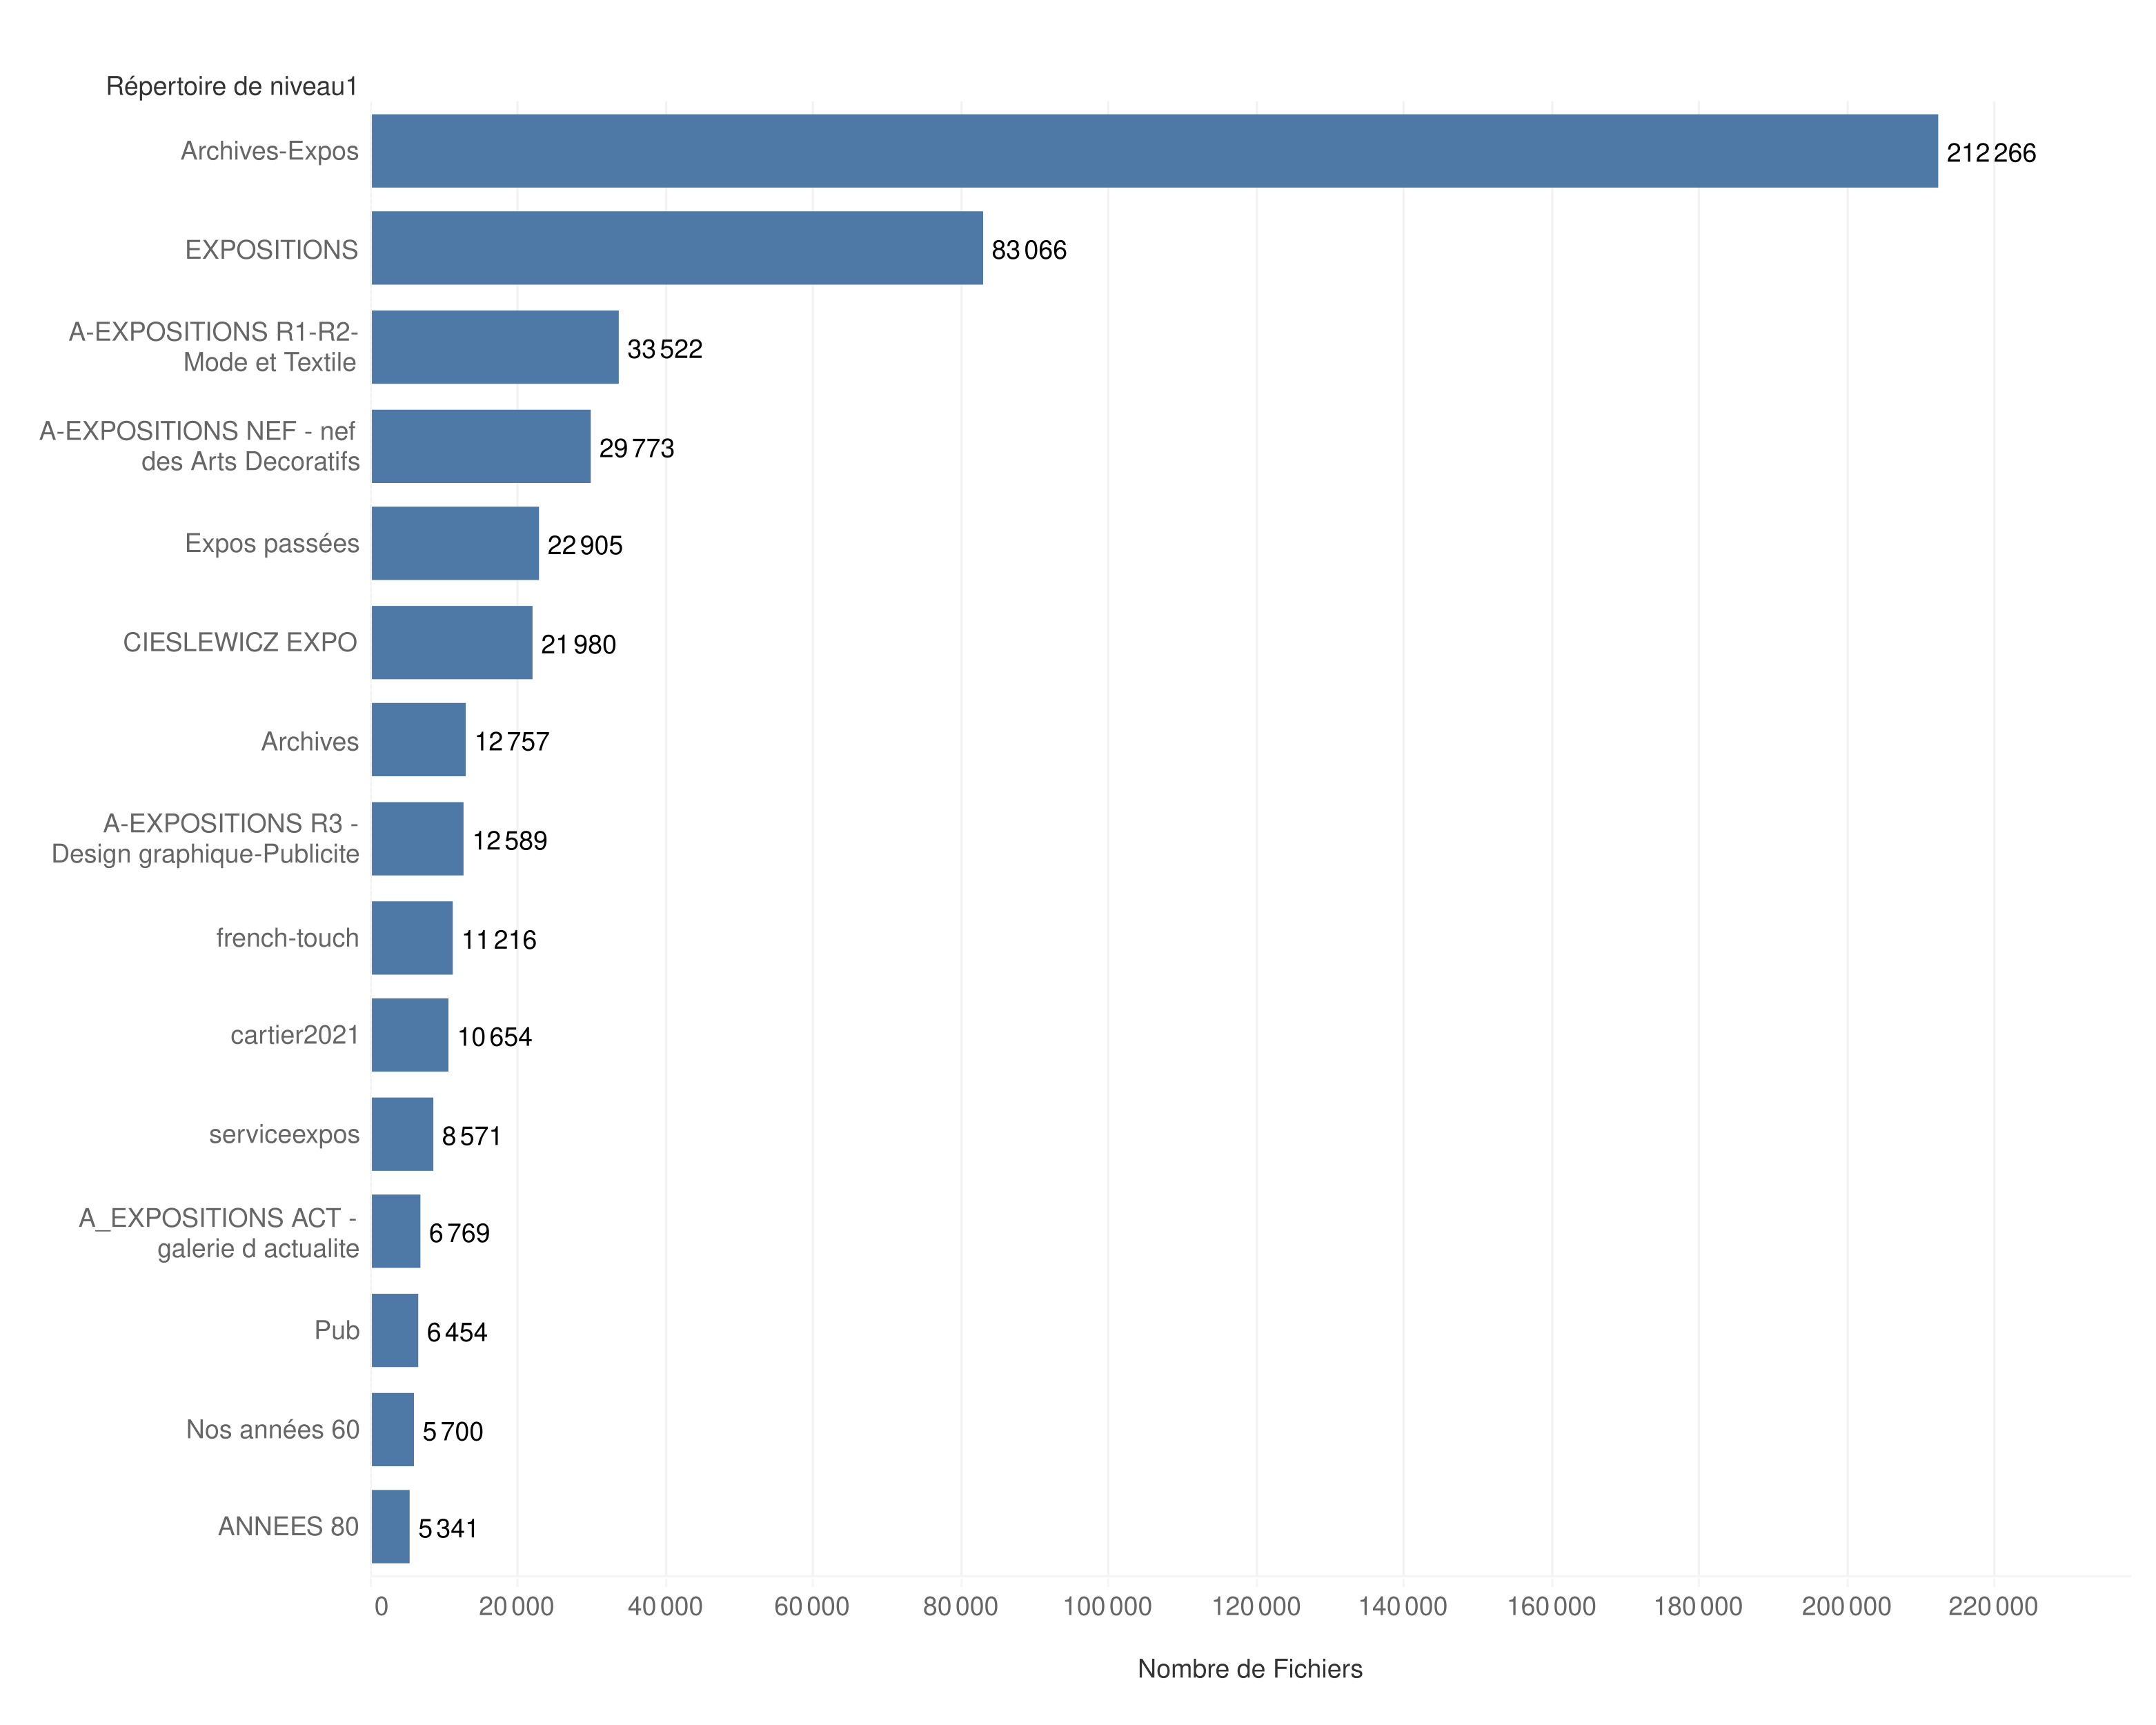
\includegraphics[width=0.9\textwidth]{Images/Repartition_15_Repertoires_Archives.png}
	\caption{Visualisation de 15 répertoires d'archives d'exposition}
	\label{fig:Repartition}
\end{figure}

Cette représentation fait apparaître une répartition inégale. Certains répertoires concentrent une part importante de fichiers, alors que d'autres sont presque vides. Cela se confirme avec les résultats du premier répertoire, \enquote{Archives-Expos} qui à lui seul totalise un nombre de 212 266 fichiers. Tandis que les autres comptent moins de la moitié de son volume. À partir de là, on observe donc une véritable concentration autour de certains espaces. Deux répertoires de même niveau hiérarchique peuvent en réalité correspondre à des masses documentaires différentes. La place qu'occupe un dossier dans l'arborescence ne peut renseigner à elle seule sur son importance quantitative. Cette analyse permet dénombre total de fichiers et leur poids : soit 553 432 pour le les fichiers et 2,43 To (téraoctets) de volumétrie totale des dossiers d'exposition compris dans les 8,43 To du serveur. 


En examinant les titres des répertoires, on observe une différence dans la logique de nommage. Certains répertoires renvoient à des espaces d'expositions (A-EXPOSITIONS NEF – nef des Arts Décoratifs,A-EXPOSITIONS R1-R2 – Mode et Textile, etc.), et d'autres à des expositions (CIESLEWICZ EXPO, french-touch, etc.). L'une des anomalies que l'audit nous permet de desceller pour comprendre un fonds.


\section{ Identification technique des fichiers du corpus}

\vspace{-0.4cm}
Au-delà de la volumétrie, la cartographie permet d'identifier les caractéristiques techniques des fichiers. Il s'agit de prendre connaissance des documents qui composent le périmètre. Le logiciel utilisé pour cette étape d'identification technique est la solution Droid-sh (\textit{Digital Record Object Identification}): il s'agit d'un outil développé par les Archives nationales britanniques, il s'appuie sur le registre PRONOM (\textit{Public Record Office and Nôm}) pour identifier les formats de fichiers à partir des signatures propres à chaque fichier. Pronom est comme une  « système d'information en ligne sur les formats de fichiers de données et leurs logiciels associés»\footnote{\cite{nationalarchives-pronom}.}.


\subsection*{Identification et diversités des formats}


L'analyse laisse voir une large diversité de formats des fichiers au sein des dossiers d'exposition. Celle-ci se justifie par la variété des activités de préparation des expositions et aux différents environnements logiciels utilisés par les producteurs. Les résultats obtenus permettent non seulement de faire une répartition par famille de formats, mais aussi d'identifier les formats prépondérants et plus largement de détecter d'éventuelles anomalies.

\begin{figure}[H]
	\centering
	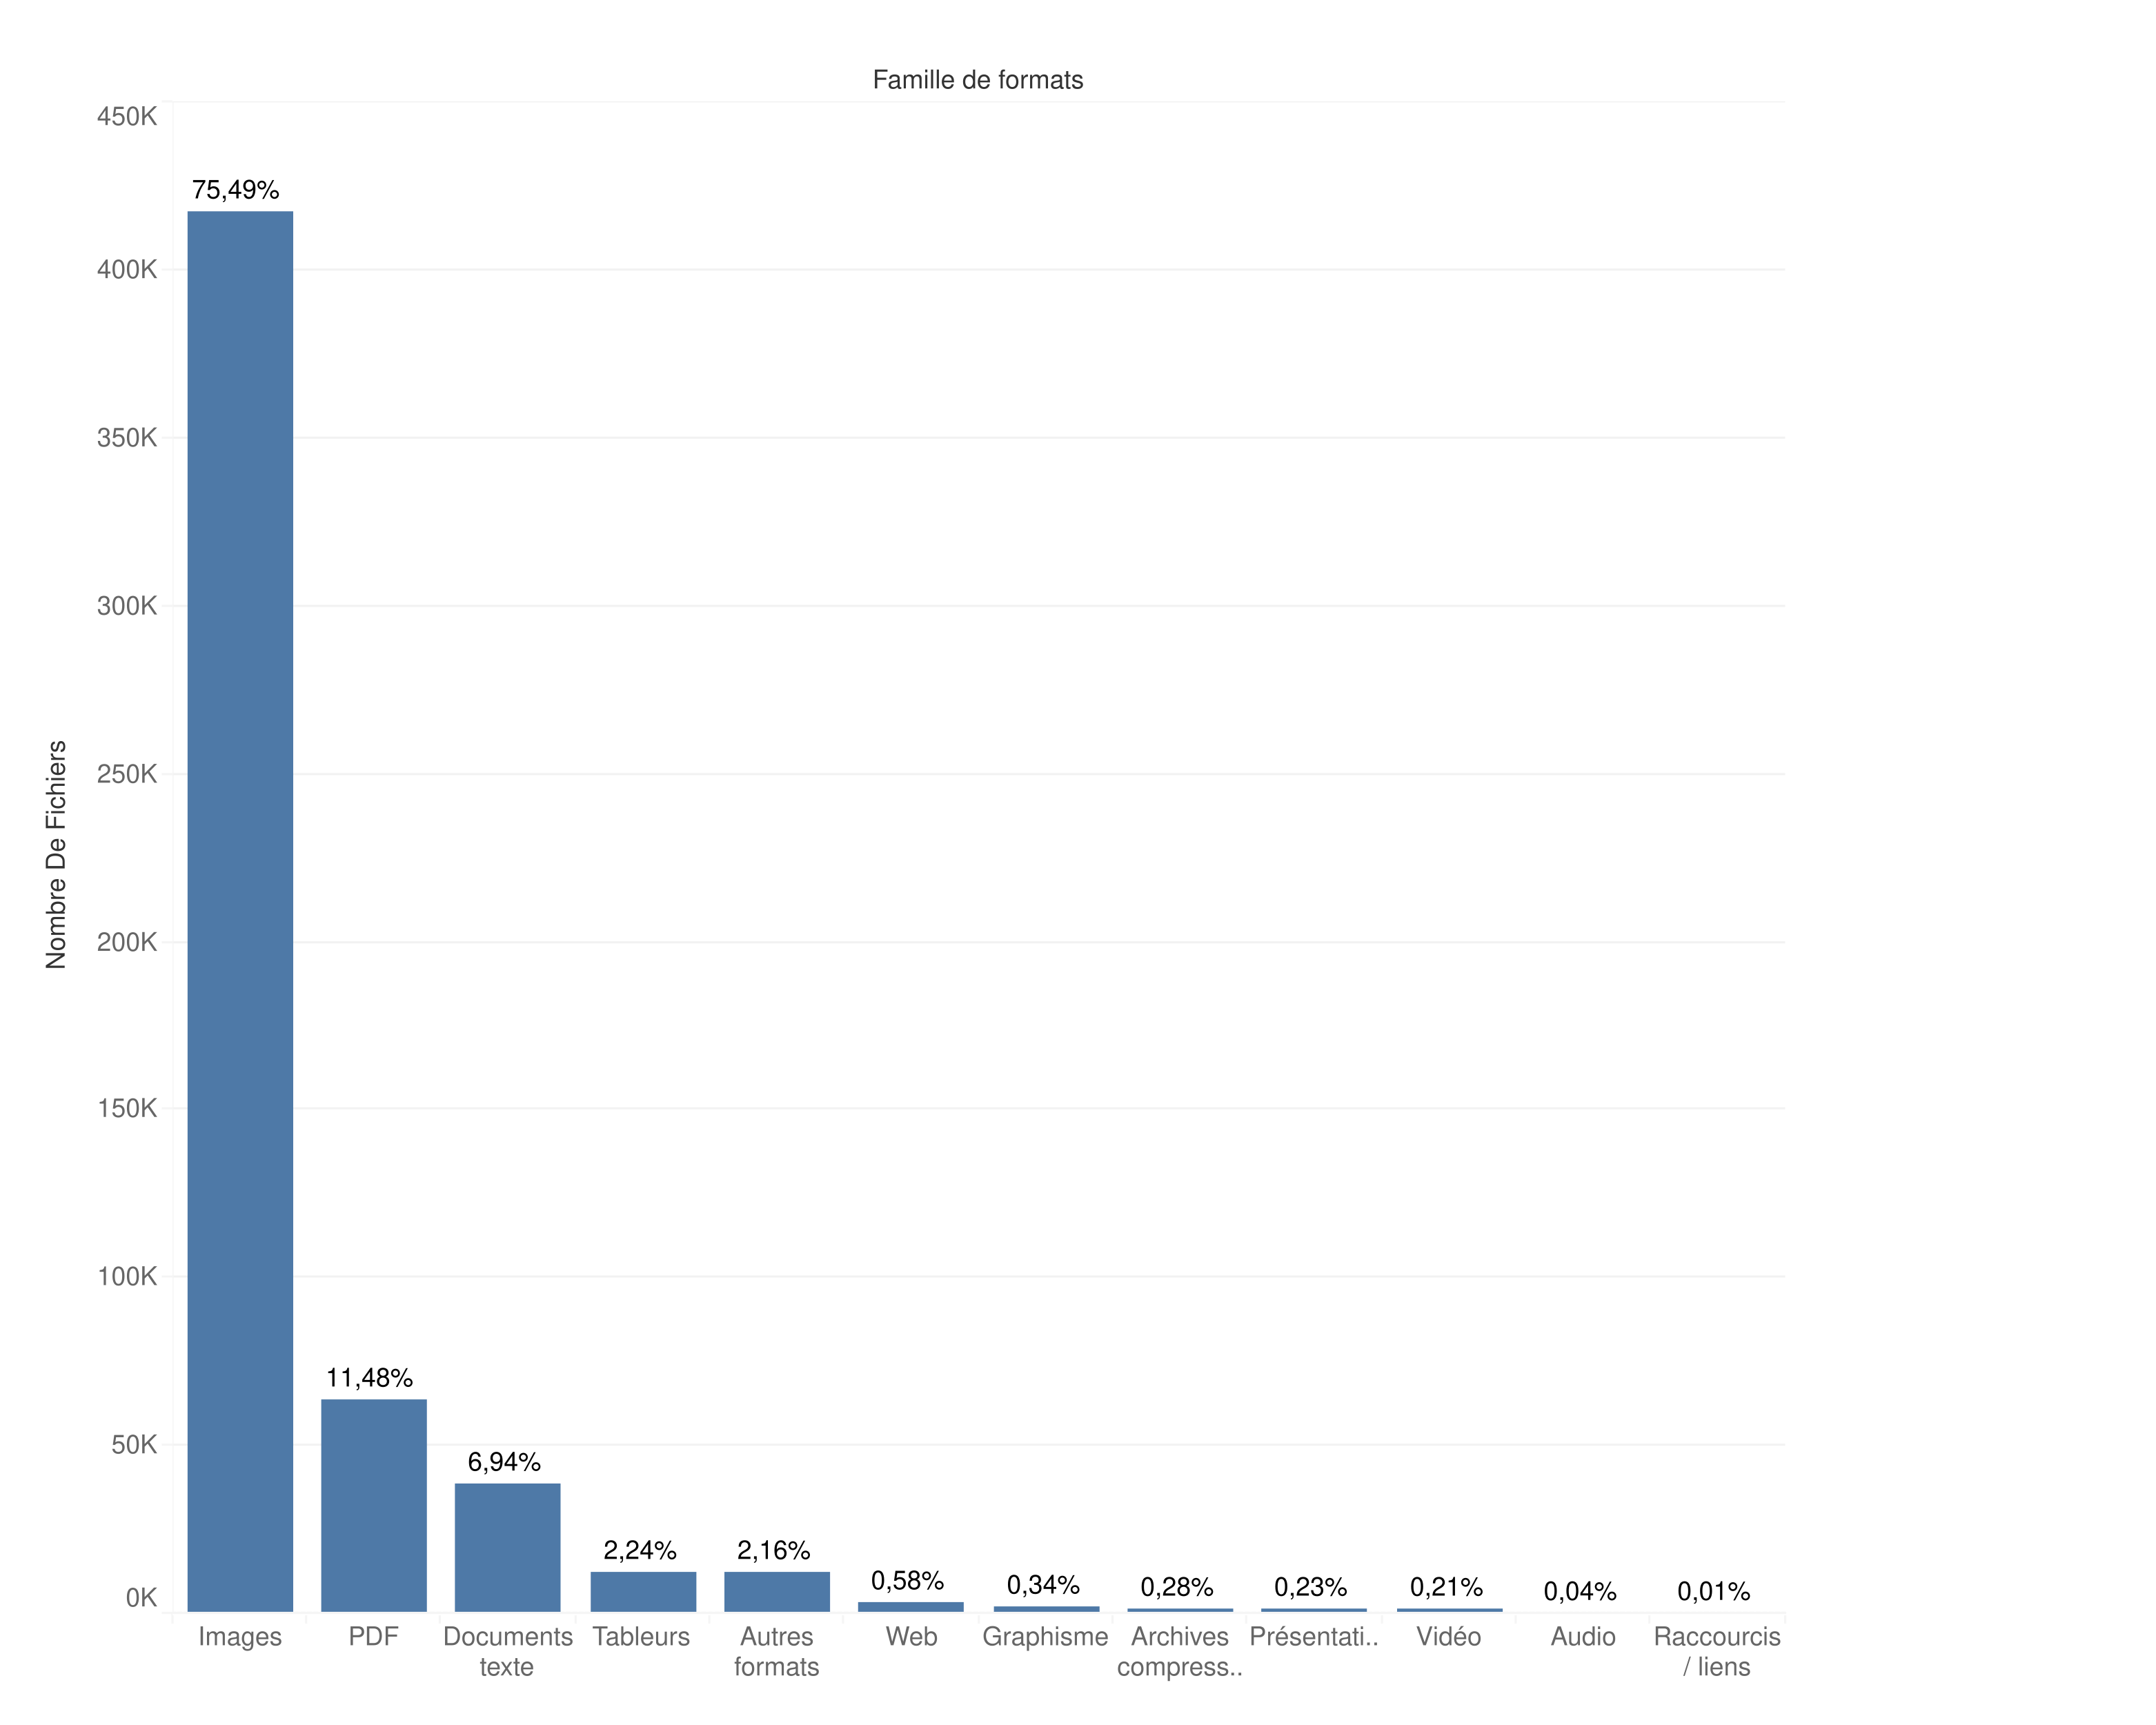
\includegraphics[width=0.8\textwidth]{Images/Repartition-Famille-Formats.png}
	\caption{Répartition des familles de formats de fichiers}
	\label{fig:Repartition-famille-formats}
\end{figure}

\begin{table}[H]
	\centering
	\renewcommand{\arraystretch}{0.5}
	\setlength{\tabcolsep}{3 pt}
	\resizebox{\textwidth}{!}{%
		\begin{tabular}{lrr}
			\toprule
			\textbf{Famille de formats} & \textbf{Nombre de fichiers} & \textbf{Pourcentage (\%)} \\
			\midrule
			Images                 & 417~782 & 75,49~\% \\
			PDF                    & 63~527  & 11,48~\% \\
			Documents texte        & 38~382  & 6,94~\% \\
			Tableurs               & 12~418  & 2,24~\% \\
			Autres formats         & 11~961  & 2,16~\% \\
			Web                    & 3~202   & 0,58~\% \\
			Graphisme              & 1~906   & 0,34~\% \\
			Archives compressées   & 1~554   & 0,28~\% \\
			Présentations          & 1~254   & 0,23~\% \\
			Vidéo                  & 1~156   & 0,21~\% \\
			Audio                  & 241     & 0,04~\% \\
			Raccourcis             & 49      & 0,01~\% \\
			\midrule
			\textbf{Total}         & \textbf{553~432} & \textbf{100,00~\%} \\
			\bottomrule
		\end{tabular}%
	}
	\caption{Répartition des fichiers du fonds par famille de formats}
	\label{tab:repartition_formats}
\end{table}

\vspace{0.5cm} % Renvoyer la ligne vers le bas	
À l'issue de l'analyse, douze familles sont identifiées au sein du fonds (voir figure~\ref{fig:Repartition-famille-formats} et tableau~\ref{tab:repartition_formats}). On observe une prédominance fulgurante des formats d'image, qui représentent à eux seuls trois quarts du volume total (75,49 \%, pour 417 782 fichiers). Les documents de gestion et de travail (PDF et documents bureautiques) représentent le second ensemble le plus représenté, tandis que les formats multimédias (images, video) et de conception graphique sont minoritaires. Les autres autres formats listés font référence aux extensions qui n'existent pas : .Administration, .graphe, .adéfinir, .service, etc. Ces extensions sont la conséquence d’un mauvais nommage qui comporte un point à la place d'un \textit{underscore} et qui résultent de l'activité métier. En effet, l'outil identifie comme extension tout ce qui suit un point. 

\subsection*{Empreinte numériques et identification des fichiers identiques}

Comme l'a montrée l'étude du vrac dans les chapitres précédents, la coexistence de plusieurs occurrences d'un fichier dans différents emplacements est dû aux modalités de travail et de stockage. Le but de l'audit ici est de pointer cette anomalie à partir d'une analyse globale.

L'empreinte numérique constitue une forme d'identifiant unique qui permettant de repérer un fichier dans un ensemble. À l'image du NIR (numéro d'inscription au répertoire de la sécurité sociale), encore appelé \enquote{numéro de sécurité sociale}, qui permet d'identifier une personne dans le système de protection sociale français, l'empreinte numérique permet de distinguer un fichier d'un autre. À cet égard, il devient important de le générer. Nous choisissons de le faire avec Droid-sh qui le faire, il calcule automatiquement à partir du contenu d'un document. Toute modification du contenu affecte le calcul, donc modifie l'empreinte. Le logiciel identifie le nombre d’occurrence des fichiers à partir de l'empreinte, indépendamment de leur nom d'origine. C'est ce qu'on appelle des fichiers identiques, les doublons. Cette notion se distingue des versions des documents ( qui représentent différentes mises à jour effectuées sur un document tout au long de son cycle de vie). 



\section{Les limites de l’audit technique face aux besoins de structuration}


L'utilisation de solutions gratuites, telles qu'Archifiltre et DROID pour la réalisation d'un audit met en lumière plusieurs aspects : l'emplacement exacte des archives d'exposition dans le serveur, leur volumétrie, leur format ainsi que leur place dans le serveur par rapport aux autres documents qui s'y trouvent. 

Même si l'audit occupe une place importante dans le processus de prise en charge d'un vrac numérique, il ne permet pas à lui seul le traitement archivistique que nous souhaitons réaliser.


\subsection*{Une identification des documents insuffisante pour leur qualification}

Le document numérique se positionne au même niveau que le document papier, c'est ce que souligne Code Civil dans son article 1366. Il mentionne que :\enquote{L'écrit électronique a la même force probante que l'écrit sur support papier, sous réserve que puisse être dûment identifiée la personne dont il émane et qu'il soit établi et conservé dans des conditions de nature à en garantir l'intégrité}\footnote{\cite{code-civil-1366}}. Comme nous l'avons mentionné plus haut, l'audit se présente comme une sorte de \enquote{carte géographique} de l'arborescence fichier à traiter, il détermine avec précision les différents endroits dans lesquels on retrouve les documents, indique la place qu'ils prennent et repère les chemins d'accès. Malgré cette vision, plusieurs points ne facilitent pas leur qualification intellectuelle et juridique.

\textbf{La limite des métadonnées techniques }  Les résultats de l'audit technique seuls ne permettent pas de qualifier juridiquement et intellectuellement les documents. En effet, le scan identifie les informations techniques telles que le format de fichiers (.pdf, .jpg, .tiff), la taille ou les dates d'enregistrement et de modification. Ces éléments ne permettent pas de déterminer la valeur de preuve d'un document (un document enregistré : Cartel-salle6, ne renseigne pas sur son importance ou sur l'obligation légale de conservation).

\textbf{Le problème de la corruption sémantique}  Le problème de nommage n'est pas le résultat d'un mauvais travail de l'archiviste, mais plutôt le résultat des pratiques non encadrées. Un fichier mal nommé rend difficile son identification mais aussi la fonctionnalité de nommage intégrée aux outils d'audit (Archifiltre). On se retrouve face à des titres non signifiant c'est-à-dire flous, avec des abréviations métiers ou des noms propres des salariés. Avec la masse importante que représente le vrac, il est primordial d'effectuer un vrai travail de contrôle après cette opération. 


\subsection*{L’absence de structuration documentaire exploitable}

En effet, en dehors de la qualification des documents, l'audit ne répond pas à une organisation du fonds. Le scan fournit est le résultat de la photographie de l'arborescence des services, celle-ci découle des pratiques quotidiennes des collaborateurs. Il résulte de là une organisation souvent anarchique et non structurée; pourquoi? Parce que leur méthode de rangement n'est pas conforme aux exigences du plan de classement de l'institution. Cette situation montre la limite des solutions utilisées, car elles ne permettent pas de créer l'arborescence métier et de ranger les documents en fonction de leur contexte.



\chapter{Développement et modélisation des solutions techniques en Python}

Une fois le corpus connu, et l'identification des caractéristiques techniques effective, on peut se demander comment faire pour rendre le vrac exploitable. C'est la question à laquelle nous avons essayé de répondre durant notre alternance au MAD. Nous avons proposé une solution, puis nous l'avons expérimenté sur un ensemble concret. Pour ce faire, nous avons conçu un prototype algorithmique qui se décline en trois phases, et basé sur des actions concrètes à partir du langage de programmation Python. 
Ce chapitre se donne donc l'objectif de présenter la chaîne de traitement du vrac numérique telle que nous l'avons proposé, d'abord une intervention sur la structure matérielle des documents dans le but de rendre accessible le contenu compressé, ensuite le tri préalable des documents par catégories, enfin leur transfert vers l'arborescence de  fichiers.

\section{Préparation des données : automatiser la décompression des fichiers}

Avant d'effectuer le traitement des dossiers d'exposition, nous avons, à partir des résultats de l'audit technique Archifiltre remarqué la présence de documents compressés. Or, il est important d'accéder à tous les documents pour garantir un traitement efficace.

\subsection*{La décompression comme préalable au traitement du fonds}

Le traitement des données, structurées ou en vrac ne peut s'opérer directement sur des données encapsulées, comme les archives compressées. La décompression ici constitue l'étape préliminaire au traitement, dans le sens où elle nous donne accès à l'ensemble des documents qu'il contient. Cette opération représente une ouverture au tri des documents : si ceux-ci ne sont pas accessibles dans leur intégralité, alors le fonds en lui-même demeure partiellement inaccessible, ce qui rend difficile le traitement. Loin d'avoir du sens uniquement dans le contexte informatique, la décompression est abordée dans le contexte archivistique. C'est ce qu'illustre la norme \textit{Preservation Metadata} : \textit{Implementation Strategies} (PREMIS) dans son vocabulaire, elle la qualifie comme le processus qui consiste à inverser les effets de la compression\footnote{\cite{loc_premis_decompression}}. En d'autres termes, c'est l'action qui donne accès aux contenus des fichiers compris dans les dossiers archives. On se rend donc compte que la décompression, même si elle ne constitue pas un traitement archivistique. Dans le cadre de notre expérimentation, elle est considérée comme une opération préalable — une réflexion matérialisée en amont pour la suite du traitement.


\subsection*{Conception du script et contrôle des opérations de décompression}

Avant d'entrer dans le vif du sujet, il convient de mentionner que les résultats d'Archifiltre mettent en évidence cinq extensions d'archives compressées dans le corpus, à savoir : .zip, .rar, .7z, .tar et .gz. L'objectif est donc d'identifier ces archives et d'extraire d'elles le contenu informationnel qu'elles comportent. Afin de matérialiser cet impératif de préparation, nous avons conçu un script Python. Il effectue le traitement de manière sécurisée sur un ensemble important de documents.
Son exécution repose sur trois actions majeures, en respectant l'objectif de traçabilité telle que présenté dans les chapitres précédents.\\[0.2cm]

\begin{itemize}[label=---]
	\item \textbf{Le repérage et l'identification de l'archive}: Le programme effectue le parcours récursif de l'arborescence fichier, dans le but de trouver les extensions d'archives sus-évoquées. Il effectue le scan sur la base des informations contenues dans le rapport d'audit de l'outil Archifiltre.
	\item \textbf{Extraction}: L'archive, une fois identifiée, est renommée. Il est question de prendre connaissance de son contenu à travers l'opération \enquote{d'extraction}. C'est elle qui constitue le cœur de la décompression. 
	\item \textbf{Le renommage}: Elle représente notre stratégie de marquage de sécurité. Elle empêche de se retrouver lors du traitement avec la même problématique d'identification et d'accès à l'information. L'archive est renommée par l'ajout de l'extension (.traite), c'est un choix pour identifier les archives déjà traitées et éviter toute autre opération de décompression sur ces documents.	
\end{itemize}

Il est important de mentionner que chaque événement de cette opération est enregistrée dans un journal (log), afin de garantir sa traçabilité.
La décompression produit donc deux types de résultats : d'une part les fichiers extraits, accessibles et prêts pour l'opération suivante, et d'autre part une information permettant de faire la distinction entre les archives déjà traitées et celles qui nécessitent encore une intervention. Cependant, cette première étape ne résous pas le problème du vrac numérique. Elle ne permet toutefois pas de déterminer si les documents sont prêt pour l'archivage pérenne. C'est pour ca qu'il convient d'aller plus loin en mettant en place un processus de catégorisation propre à l'opération de tri.


\section{De la masse documentaire à la catégorisation automatisée}

C’est le cœur archivistique de notre développement. À la suite de la préparation des données, nous cherchons désormais à catégoriser les fichiers. Ce mécanisme se matérialise par l'opération de tri, en d'autres termes, l'extraction des données qui entrave le corpus.

\subsection*{Identification des éléments à écarter au traitement}

Dans sa réflexion sur le vrac numérique, Marie-Anne Chabin veut nous montrer que le tri numérique nécessite une qualification rigoureuse des documents. Elle veut aussi nous faire comprendre que cette opération n'est pas juste chercher à ordonner un désordre à posteriori, mais plutôt une anticipation ou une préparation des documents à leur conservation future\footnote{\cite{chabin-vrac-2016}}.

La solution inclut l'identification des données qui polluent le périmètre étudié. Ces données se répartissent donc en plusieurs catégories distinctes. Cette opération résulte de l'analyse scrupuleuse des résultats de l'outil Droid.\\[0.1cm]

\textbf{Les éléments issus de la décompression} : Le script identifie les archives traitées en amont avec le nouvel extension .traite, qu'il range dans la catégorie \enquote{Archives}.

\textbf{Les éléments à utilité temporaire} : Ici, le programme parvient à identifier les données de sauvegarde (.tmp, .bak, .wbk), les données de configuration (.ini, .inf, .dat), celles issues d'une recherche internet (.aae, .pc3, .url) et les polices (.ttf, .otf, .ttc).

\textbf{Les éléments qui ne contiennent pas de données documentaires exploitables} : Il s'agit tout simplement des fichiers ou répertoire de fichiers vides.

\textbf{Les éléments en double} : Selon la méthode d'identification par l'empreinte numérique de chaque document, car elle permet d'identifier leurs doublons exacts\footnote{\cite{bnf_integrite_donnees_numeriques}}. Le prototype parvient à repérer dans l'ensemble du corpus étudié les informations répétées et invisibles à l’œil nu.

Cette qualification est effectuée sur la base de la nature des documents. Notre logique de traitement s'appréhende dans le tableau suivant : 

\begin{table}[h]
	\centering
	\renewcommand{\arraystretch}{1.5}
	\setlength{\tabcolsep}{10pt}
	\resizebox{\textwidth}{!}{%
		\begin{tabular}{lp{10cm}}
			\toprule
			\textbf{Catégorie identifiée} & \textbf{Pourquoi l'isoler ?} \\
			\midrule
			Les éléments issus de la décompression (.traite) & Traces des archives traitées en amont \\
			Les éléments à utilité temporaire & Composants logiciels, graphiques et informatiques, ou coquilles vides de sens (liens) \\
			Fichiers/dossiers vides & Absence de contenu \\
			Doublons & Contenu identifié comme identique à un autre \\
			\bottomrule
		\end{tabular}%
	}
	\caption{Présentation des catégories de données triées}
	\label{tab:categories_tri}
\end{table}


\subsection*{mise à l’écart contrôlée : constitution d’un répertoire des éliminables}

Au lieu de supprimer directement le flux d'informations qui polluent l'ensemble à traiter, le script se propose de créer un répertoire de mise en quarantaine de ces données. 
Tout comme les archives institutionnelles papiers, les archives institutionnelles numériques ne peuvent faire l'objet d'une élimination en amont par l'archiviste. C'est dans ce contexte que se situent les archives numériques d'exposition. La décision d'élimination archivistique doit être validée par l'autorité étatique qui a la charge du contrôle scientifique et technique sur la gestion des archives du MAD. Pour des mesures de sécurité et de prudence, l'algorithme crée un dossier dont le but est de proposer les documents à élimination. Ce répertoire fait office d'espace intermédiaire entre l'identification automatique et la décision d'élimination définitive.

L'arborescence générée par le script est organisée en fonction des différentes catégories sus-identifiées, leur création est faite sous la forme de sous-dossiers. Cette organisation permet non seulement de se retrouver dans un bruit informationnel, d'écarter les anomalies des données saines qui doivent faire l'objet d'un classement ultérieur, mais surtout, elle rend possible la vérification humaine. C'est là que notre choix de l'automatisation comme mesure d'assistance au raisonnement humain prend du sens. On voit bien qu'à partir de cette vérification, l'humain (archiviste), peut réellement identifier les forces et les faiblesses de l'outil, en vérifiant s'il récupère avec exactitude les extensions de fichiers définis dans la règle.


\section{Reconstitution de l’arborescence cible}

Avant de rentrer dans l'exposé de notre argumentaire, il convient de préciser que quelques modifications visuelles et structurelles ont été apportées au plan de classement initial de l'institution. Avec l'approbation de l'archiviste, nous avons rajouté une numérotation (01, 02, 03 etc.) afin de permettre au programme de se retrouver plus facilement dans la création de l'arborescence : cette opération ne modifie en rien sa structure et son contenu. 

En outre, la reconstitution du plan de classement représente une tâche importante pour l'opération de traitement, car il s'agit de reproduire la même structure pour faire correspondre les données saines au dossier de l'activité qui l'a produite.


\subsection*{formalisation des règles sémantiques et de l'arborescence cible}

Le troisième script constitue l'étape de fin, liée à la réorganisation intellectuelle du vrac. Il s'agit de déterminer la destination dans le plan de classement. 

Pour que le programme fonctionne, il convient de lui faire comprendre les règles documentaires que nous aimerions appliquer. Si on prend le cas, par l'exemple, d'un humain qui sait à partir du nom d'un fichier nommé \enquote{Prêt} que celui-ci rentre dans la partie réservée au prêt, ce n'est pas le cas d'un l'algorithme informatique. L'objectif pour nous est de lui faire comprendre le jargon métier et de lui montrer où il doit affecter les documents sur la base des informations qu'il dispose. C'est pour cette raison que nous avons conçu un dictionnaire de synonyme métier. Celui-ci récapitule les mots couramment utilisés par les agents et leurs dérivés (abréviations et synonymes). Pour que les règles soient correctement comprises, nous sommes passer par la normalisation textuelle : qui consiste à un nettoyage des mots (suppression des accents via \textit{unicodedata}, uniformisation des caractères, conversion des majuscules en minuscules, remplacement des tirets et des underscores par des espaces). Cette opération permet d'avoir les informations au même niveau de compréhension et d'éviter des erreurs de variation typographique. 

La stratégie décisionnelle est simple, le script applique un ordre logique au processus de transfert. D'abord le transfert à partir des mots-clés du plan du classement et du dictionnaire métiers présents dans le nommage du fichier ou son répertoire parent (principe d'héritage), ensuite, le transfert à partir des règles de nommage de la photothèque, et un transfert par l'analyse du contenu des fichiers et le scan du dictionnaire métier.

\subsection*{Fonctionnement du script}

Le fonctionnement du script s'articule autour de plusieurs briques logicielles complaisantes assurant l'analyse, le classement intelligent et sécurisé des documents. Pour se faire nous passons par : 


\textbf{L'extraction multi-formats} : Le script est capable d'effectuer la lecture dynamique du contenu textuel de divers types de documents dans le but d'alimenter l'analyse sémantiques (documents bureautiques et présentation via python-docx et python-pptx, les tableaux via pandas/odf, les fichiers PDF via une double analyse, \textit{pdfplumbe}r pour une analyse fine et pypdf dans la mesure où l'option précédente n'a pas marché).\\[0.1cm]

\textbf{Le moteur de classement en deux phases} : Deux phases déterminent le classement des documents dans l'arborescence : le tri de surface et l'analyse sémantique.

\begin{itemize}[label=---]
	\item \textbf{Phase 1 (tri de surface)} : Il s'agit de l'analyse des mots-clés identifiés dans le nommage des documents, la détection des codes de nomenclature spécifiques tel que les codes définit par la photothèque), et l'héritage de correspondance du dossier parent.
	\item \textbf{Phase 2 (analyse sémantique) }: Le script utilise un système de \textit{scroring}, qu'il tente d'appliquer à cette deuxième phase. Le but étant d'extraire le contenu des documents (texte), de faire une comparaison avec le dictionnaire de mots-clés préalablement constitué par l'archiviste et comportant les différentes expressions liées à l'activité d'exposition et leurs déclinaisons. 
\end{itemize}


Afin d'assurer la sécurité des données transférées, et de garantir la conservation des métadonnées propres des documents, nous effectuons la copie à partir de la fonction \textit{copie-file}. Les métadonnées suivantes sont conservées : les dates de création, le nom de l'auteur, la/les dates de modification (pour justifier les différentes opérations effectuées sur lui). 

Dans l'optique de vérifier que le prototype prend en considération les règles prédéfinies dans les trois niveaux, nous l’appliquons dans le chapitre suivant à un corpus réel.


\chapter{Exécution de la chaîne de traitement, évaluation critique et perspectives institutionnelles}

Le déploiement d'une solution représente la principale solution que nous avons développée pour pallier le problème des dossiers d'exposition éclatés. Cette approche en triplet est le fil conducteur qui permet de passer d'une expérimentation théorique à une réalisation concrète et mesurable. Nous organisons notre argumentaire dans ce chapitre en trois temps. D'abord la mise en œuvre à travers des étapes successives d'analyse, de structuration et de transfert automatisé des documents vers une arborescence cible au sein du MAD. Puis la concrétisation de la solution sur un jeu de données réel, regroupant toutes les caractéristiques d'un dossier d'exposition. Enfin,  nous soumettrons les résultats obtenus à une évaluation critique approfondie, en présentant les limites techniques et méthodologiques de notre projet.


\section{Mise en œuvre de la chaîne de traitement sur un corpus expérimental}

Pour expérimenter notre solution, nous avons sélectionné des dossiers d'exposition et appliquer successivement nos trois scripts.



\subsection*{Sélection d’un échantillon d’expérimentation}


Dans le but de faire valoir la robustesse de notre chaîne de traitement automatisé, nous n'avons pas mené notre expérimentation sur l'intégralité des dossiers d'exposition du serveur YODA, mais plutôt sur une sélection minutieuse de dossiers menée en concertation avec l'archiviste. Cette angle de traitement permet de tester le prototype sur des volumes hétérogènes et représentatifs de la réalité institutionnelle. Pour ce faire, l'échantillon se compose des ensembles suivants : 

\textbf{Le dossier d'exposition globale \enquote{Cieslewicz-Expo}} : Sélectionné par l'archiviste pour cas d'étude de référence, parce qu'on retrouve l'ensemble des typologies documentaires et composantes types qu'on retrouve dans un dossier d'exposition dit complet. Il représente une volumétrie initiale de 21 980 fichiers. Selon le rapport d'audit d'Archifiltre, il constitue l'exposition (de niveau 1) la plus volumineuse.

\textbf{Les expositions \enquote{French-touch} et \enquote{Cartier2021}} : Elles font de notre sélection, pour tester le comportement de l'algorithme sur un volume documentaire intermédiaire, entre 11 216 et 10 654 fichiers.

\textbf{Le dossier d'exposition \enquote{Bauhaus}} : Il s'agit d'une sélection stratégique de l'archiviste pour assurer le contrôle qualité final. De prime abord, nous avons localisé 1996 fichiers dans le répertoire de niveau 1 (le dossier d'exposition lui-même), qui, une fois enrichis de l'ensemble des fichiers appartement à cette exposition dans les autres répertoires de YODA (presse, service des expositions, etc.), comptabilise comptabilisons au total 15 284  fichiers.  

\vspace{-1.9cm} % Pour faire monter le texte
\subsection*{Exécution réelle du transfert et préservation des données}

À la suite de la définition du périmètre de l'échantillon, le service informatique a mis à notre disposition un espace dédié. Nous avons exécuté les trois scripts les uns à la suite des autres. Cette phase se déroule en trois temps successifs, chacun répondant à un objectif précis de traitement du fonds en vrac comme nous l'avons vu dans le chapitre 8.

\textbf{Premier temps (décompression)} : Le premier script nous a permis de scanner l'ensemble des répertoires afin d'identifier et extraire les archives compressées. Il applique le marqueur (.traite), afin d'éviter une redondance de traitement, le script ne tarde pas à consigner tout événement dans le journal de traçabilité dédié. L'image ci-dessous illustre de l'application concrète de ce marquage (avec l'extension \textit{.traite}) sur les archives décompressées, permettant ainsi de garantir le suivi de l'exécution du script avant le basculement des documents vers l'arborescence cible.

\begin{figure}[H]
	\centering
	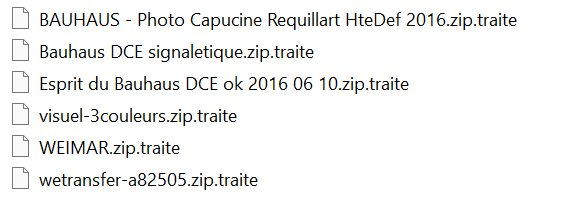
\includegraphics[width=0.8\textwidth]{Images/Decompression.jpeg}
	\caption{Vue rapprochée du renommage des archives compressées après exécution du script}
	\label{fig:Decompression}
\end{figure}

\textbf{Deuxième temps (tri et constitution d'un répertoire des éliminables)} : À partir de la croisée des données issues des exports de l'outil Droid, ce script effectue une opération chirurgicale sur les échantillons, il les nettoie et isole automatiquement les fichiers ou dossiers n'ayant aucun intérêt pour le fonds, notamment, les fichiers vides, temporaires, les doublons (à partir de la détection et la comparaison de l'empreinte numérique MD5) des fichiers sains.

\begin{figure}[H]
	\centering
	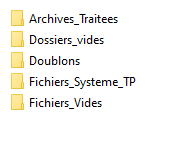
\includegraphics[width=0.8\textwidth]{Images/Arbo_Tri.PNG}
	\caption{Visualisation de l'arborescence de tri}
	\label{fig:Tri}
\end{figure}

\vspace{0.5cm} % Pour faire descendre le texte
\textbf{Troisième temps (transfert vers l'arborescence cible)} : Enfin, le troisième script parcourt les dossiers et fichiers sains qu'il transfère automatiquement l'arborescence institutionnelle de classement, c'est la fonction principale de notre traitement. À ce niveau, on peut se demander sur quelle base le transfert s'est opéré? La réponse est simple, l'algorithme reconstruit intégralement la structure du plan de classement. Pour rendre le transfert effectif, il se subdivise en deux points. Le premier se base sur une comparaison des synonymes qu'il récupère dans la colonne typologie, du dictionnaire de synonymes métiers en combinant au tri de surface (une comparaison avec le titre du fichier, à partir de l'héritage du dossier parent et les initiales des identifiants de la photothèque pour permettre l'identification d'images). Le second porte sur l'analyse sémantique textuelle pour les documents qui n'ont pas pu être traités en amont de l'opération. 

\begin{figure}[H]
	\centering
	\includegraphics[width=0.8\textwidth]{Images/Arbo-fichiers.png}
	\caption{Vue de l'arborescence de destination structurée générée automatiquement}
	\label{fig:Arborescence}
\end{figure}

 
Tout au long des différents transferts que nous avons effectué, la préservation des données est sécurisée par l'utilisation de la fonction de copie sécurisée : \textit{shutil.copy2()}. L'idée est de préserver les métadonnées d'origine des fichiers transférés, telles que la date de modification, les dates d'accès, les permissions. Toutefois, si l'algorithme rencontre un problème lié aux d'accès, il bascule en \textit{shutil.copyfile()}, qui copie le contenu des documents (date de création, auteur, date de modification, titre, etc.) qu'on retrouve généralement dans les détails des propriétés propres à ceux-ci. Ces données sont toutes aussi importantes pour assurer leur archivage pérenne. Nous avons eu l'exemple : Contenu créé : 18/07/2017 11: 30; ce qui représente la date d’origine de l’archive, inscrite directement dans la structure du document.

\section{Résultat et évaluation critique du traitement automatisé}

Une fois que nous avons appliqué les scripts à un ensemble réel, nous nous proposons dans cette partie de faire une analyse concrète sur le taux de réussite des différents scripts. Cette démarche se décline en deux parties : d'abord une évaluation quantitative, et ensuite une analyse des réussites ainsi que des erreurs.

\subsection*{Évaluation quantitative des trois étapes de traitement}

Nous détaillons notre analyse en trois temps :

\begin{table}[H]
	\centering
	\renewcommand{\arraystretch}{1.5}
	\setlength{\tabcolsep}{10pt}
	\resizebox{\textwidth}{!}{%
		\begin{tabular}{lrrr}
			\toprule
			\textbf{Dossier d'exposition} & \textbf{Nombre de fichiers} & \textbf{Archives décompressées} & \textbf{Taux de réussite} \\
			\midrule
			Cieslewicz-Expo & 21~980 & 100 & 100~\% \\
			French-touch    & 11~216 & 0   & --- \\
			Cartier2021     & 10~654 & 17  & 100~\% \\
			Bauhaus         & 15~284 & 468 & 100~\% \\
			\midrule
			\textbf{Total} & \textbf{59~134} & \textbf{585} & \textbf{100~\%} \\
			\bottomrule
		\end{tabular}%
	}
	\caption{Résultats de l'étape 1 -- décompression}
	\label{tab:etape1_decompression}
\end{table}


Le script parvient à appliquer correctement les trois temps de traitement sur les fichiers sélectionnés : détecter, décompresser et renommer.

\begin{table}[H]
	\centering
	\renewcommand{\arraystretch}{1.5}
	\setlength{\tabcolsep}{10pt}
	\resizebox{\textwidth}{!}{%
		\begin{tabular}{lrrrr}
			\toprule
			\textbf{Dossier d'exposition} & \textbf{Nombre de fichiers} & \textbf{Fichiers sains} & \textbf{Fichiers éliminables} & \textbf{Taux de réussite} \\
			\midrule
			Cieslewicz-Expo & 21~980 & 19~567 & 2~413 & 100~\% \\
			French-touch    & 11~216 & 5~026  & 6~190 & 100~\% \\
			Cartier2021     & 10~654 & 7~295  & 3~759 & 100~\% \\
			Bauhaus         & 15~284 & 7~117  & 8~167 & 100~\% \\
			\midrule
			\textbf{Total} & \textbf{59~134} & \textbf{39~005} & \textbf{20~529} & \textbf{100~\%} \\
			\bottomrule
		\end{tabular}%
	}
	\caption{Résultats de l'étape 2 -- tri}
	\label{tab:etape2_tri}
\end{table}

Comme le montre le tableau ci-dessus, l'algorithme parvient non seulement à écarter les fichiers sains des autres fichiers en les rangeant dans le dossier des éléments éliminables et les répartissant par catégories\footnote{Voir figure~\ref{fig:Tri}}.


\begin{table}[H]
	\centering
	\renewcommand{\arraystretch}{1.5}
	\setlength{\tabcolsep}{10pt}
	\resizebox{\textwidth}{!}{%
		\begin{tabular}{lrrr}
			\toprule
			\textbf{Dossier d'exposition} & \textbf{Correctement classés} & \textbf{Non classés} & \textbf{Taux de réussite} \\
			\midrule
			Cieslewicz-Expo & 19~471 & 96 & 99,51~\% \\
			French-touch    & 4~958  & 68 & 98,65~\% \\
			Cartier2021     & 7~285  & 10 & 99,86~\% \\
			Bauhaus         & 7~077  & 40 & 99,44~\% \\
			\midrule
			\textbf{Total} & \textbf{38~791} & \textbf{214} & \textbf{99,45~\%} \\
			\bottomrule
		\end{tabular}%
	}
	\caption{Résultats de l'étape 3 -- transfert vers l'arborescence cible}
	\label{tab:etape3_transfert}
\end{table}

Ici, l'algorithme arrive à transférer les fichiers sains retenus vers l'arborescence cible. Lors du test, nous avons constaté que le taux de réussite s'élève à 99,45~\%. Pour des raisons de sécurité, les fichiers non classés s'insèrent sous l'arborescence générée. Pour trouver le pourcentage de réussite par dossier racine traité, nous avons additionné le nombre de fichiers correctement classés par le nombre de fichiers non classés, puis divisé par le nombre de fichiers correctement classés et nous avons multiplié le résultat par 100.


\subsection*{Analyse quantitative des réussites, erreurs et écarts de catégorisation}

Les résultats mentionnés dans la section précédente nous interpellent et suscitent en nous quelques interrogations. D'abord, pourquoi y a-t-il un écart dans le traitement? Comme nous pouvons le voir, les deux premiers scripts fonctionnent à 100~\%, alors que le script de classement lui présente un taux de réussite moins élevé. Les deux premières opérations se déroulent bien tout simplement parce qu'elles se concentrent sur une analyse technique. Elles s'appuient uniquement sur les extensions de fichiers préalablement définis dans le fichier de configuration à partir de l'export Droid\footnote{Voir annexe~\ref{annexe:documentation-scripts}}. L’algorithme de transfert repose, quant à lui, sur une analyse beaucoup plus spécifique, à travers la comparaison des du contenu des fichiers. Ensuite, dans l'étape 3, pourquoi le taux d'erreurs varie selon le dossier racine? La logique de traitement ne dépend pas de la volumétrie du dossier à traiter, mais plutôt du nommage des fichiers traités et des résultats de l'analyse sémantique. Enfin, que deviennent les fichiers non classés? On remarque que 214 fichiers sur les 39 005 sains n'ont pas pu être classés. Ils sont donc rangés sous l'arborescence au même titre que les catégories du plan de classement. Cette logique peut sembler polluer l'arborescence, au contraire permet de faire un contrôle sur la qualité du traitement.

La phase d'expérimentation a nécessité plusieurs itérations algorithmiques, afin de corriger progressivement les limites techniques rencontrées lors de l'exécution des tests\footnote{Voir annexe ~\ref{annexe:journal-tests}}.

\section{Limites et conditions de poursuite du dispositif}

Cette partie dresse l'état des lieux des contraintes rencontrées sur le plan technique et des conditions requises pour assurer la pérennité de l'outil. Nous pouvons identifier la marge d'amélioration opérationnelle sans juger de la portée générale des résultats.


\subsection*{Limites techniques et méthodologiques révélées par l'expérimentation}

Cette analyse met en lumière des limites, liées aux phases de tri et d'arborescence. Premièrement, le traitement automatisé présente une anomalie : une copie du dossier des éliminables se crée dans l'arborescence du dossier racine, ce qui nécessite l'intervention humaine avant l'exécution du prochain script. Deuxièmement, le traitement physique de mise en arborescence des fichiers se heurte à des difficultés sémantiques. Le script ne classe pas les dossiers de manière uniforme, car le vocabulaire standardisé peut changer en fonction des expositions, et parce que nous n'avons pas adapté une structure de détection plus rigoureuse, compte tenu de la non uniformisation de la structure des documents en fonction de la typologie dans l'institution. 

\subsection*{Conditions de réutilisation et d’évolution du dispositif au sein du pôle Archives}

Afin de garantir l'utilisation pérenne de nos trois codes pour les archivistes du MAD, nous proposons une documentation qui explique les prérequis à mettre en place avant l’exécution jusqu'à leur application sur les dossiers d'exposition\footnote{Voir annexe~\ref{annexe:documentation-scripts}}. L'environnement de traitement dans lequel les programmes tournent est pensé pour permettre leur l'utilisation et leur compréhension par l'archiviste avec ou sans compétences techniques informatiques\footnote{Voir annexe~\ref{annexe:documentation-scripts}}. 
Cette approche permet aussi à travers les explications sur les éléments à renseigner dans le fichier de configuration. C'est aussi à ce niveau que nous montrons qu'il est important de prendre connaissance du vocabulaire de chaque exposition et renseigner dans la configuration\footnote{Voir annexe~\ref{annexe:documentation-scripts}}.\\[0.1cm]

En plus de la documentation, la réutilisation du dispositif repose sur la séparation entre le moteur de traitement et les règles métier, regroupées dans un même module de réglages. Celle-ci permet d'adapter le traitement à une nouvelle exposition, ainsi que de conformer le prototype à une éventuelle évolution des pratiques professionnelles. \\[0.1cm]

% Bout de code Python
\begin{lstlisting}[
	language=Python,
	captionpos=b,
	caption={Extrait du script de configuration \texttt{config.py}},
	label={lst:config}
	]
	# --- REGLAGES D'UNE NOUVELLE EXPOSITION ---
	dossier_racine = ""
	csv_file = "Export_Droid.csv"
	
	# Bareme des scores pour l'analyse semantique
	SCORE_MOT_CLE_TITRE = 90     # Mot-cle dans le nom du fichier
	SCORE_MOT_CLE_CONTENU = 30   # Mot-cle dans le texte
	SCORE_MAITRE_TITRE = 60      # Concept metier dans le titre
	SCORE_SYNONYME = 50          # Synonyme metier dans le titre
\end{lstlisting}


Le script complet de configuration est disponible dans le dépôt GitHub\footnote{Voir annexe~\ref{annexe:livrables-scripts-python}}. À partir de là, l'archiviste n'a pas besoin de modifier le corps de l'algorithme des scripts, il lui suffit juste d'ajouter de nouvelles variables dans le dossier de configuration.




% ----------- Conclusion --------

\chapter*{Conclusion}
\markboth{\small\textit{Conclusion}}{} %Rajout manuelle du mot conclusion en entête de la page de la conclusion
\addcontentsline{toc}{chapter}{Conclusion}
%%%%%%%%%%% Conclusion %%%%%%%%%%%%%


Au terme de notre alternance aux Arts décoratifs (MAD), nous avions pour objectif d'apporter une solution permettant de pallier au problème du \enquote{vrac numérique}, qui représente l'une des principales préoccupations des archivistes et les autres utilisateurs du serveur. L'accumulation des informations dans l'espace de stockage affecte directement l’intelligibilité et la pérennité du patrimoine institutionnel. On remarque donc que \enquote{les défis posés par la gestion de grandes quantités de données numériques exigent de nouvelles approches computationnelles permettant le traitement et l'accès aux données}\footnote{\cite{saad2026intelligence} p. 83.}. En outre, seule l'utilisation de la méthode traditionnelle de traitement archivistique ne permet pas de répondre aux enjeux liés à la résolution de ce phénomène : c'est ce que notre recherche a cherché à démontrer. Nous interrogeons la manière dont l'expertise archivistique, l'audit technique de l'espace de stockage et le recours au traitement algorithmique se croisent. Notre travail met en lumière l'alliance entre ces trois dimensions pour redonner du sens à la masse que représente le vrac.\\[0.1cm]

La mise en place d'un système d'automatisation des tâches avec scripts Python nous aide à décompresser, trier et ranger les fichiers dans le plan de classement de l'institution. Nous avons donc conçu cet outil, pour qu'il reflète nos pratiques documentaires. Son but est de montrer qu'il est tout à fait possible pour l'archiviste de se confronter aux défis du traitement massif des archives numériques alliés aux défis du traitement automatisé. Il faut comprendre par là que le programme informatique lui seul ne dispose pas d'un intérêt patrimonial s'il n'est pas guidé par la réflexion de l'archiviste. Il contribue à la transformation d'un espace de stockage en un fonds d'archives structuré et exploitable. Cela témoigne de l'évolution du métier l'archiviste au XVIe siècle, désormais confronté à problématique liées à la fois au traitement et à l'accès à l'information.\\[0.1cm]

Notre recherche a pour but de montrer l'évolution profonde du métier de l'archiviste et de ses pratiques. Toutefois, même face au recours des nouveaux outils de traitement technologique, ceux-ci ne le remplacent pas. On peut penser qu'en automatisant ses tâches on n'a plus forcément besoin de l'humain. En pratique, c'est le contraire parce que les règles de conformités sont entièrement rédigées par l'humain. L'archiviste effectue le contrôle qualité pour s'assurer de sa bonne exécution.\\[0.1cm]

Pour démontrer de façon pratique le rapport de complémentarité des trois notions évoquées, nous sommes passés par un traitement en triplet : partant de l'audit technique des dossiers exposition, en passant par la conception des scripts Python et tout ceci encadré par notre réflexion archivistique. Nous avons appliqué cette approche à un corpus réel de dossiers d'exposition. Ce qui nous a permis de nous assurer de l’exactitude du respect des règles prédéfinies par l'humain au programme, mais aussi d'ajuster et de valider notre réflexion. De plus, le fait pour d'avoir fait des erreurs nous a permis de rendre le traitement plus robuste et ciblé. 

Pour conclure, notre propos, nous pouvons dire que cette expérimentation au MAD va au-delà d'un simple exercice technique. Elle constitue le moyen de confronter la théorie archivistique à la réalité opérationnelle des grands espaces de stockage : il est donc tout à fait possible de concevoir des outils sur-mesure adaptés à des cas particuliers. Le prototype mis en place permet à l'institution de mieux préparer les données avant leur transfert sous la forme de SIP vers le système d'archivage dédié. Il peut être appliqué à tous les cas d'études, pourvus qu'ils soient confrontés aux problèmes de masse documentaire mal organisée.







\newpage{\pagestyle{empty}\cleardoublepage}



%%%%%%%%%%%%%%%%%%

\appendix %Des appendices: tables figures, etc

\cleardoublepage
\addcontentsline{toc}{chapter}{Annexes}
\appendix % Des annexes : tableaux, figures, etc.

\chapter{Livrables techniques}
\label{annexe:livrables-scripts-python}

Les scripts développés dans le cadre de ce travail sont disponibles dans le dépôt GitHub associé au mémoire. Ils sont présentés ci-dessous selon leur fonction dans le processus de traitement automatisé.

\begin{itemize}[label=-]
	\item \textbf{Script de configuration} :
	\url{https://github.com/Letis-mvg/Memoire_TNAH_2026/blob/main/Scripts_Rendus/config.py}\\[1 cm]
	
	\item \textbf{Script de décompression des fichiers} :
	\url{https://github.com/Letis-mvg/Memoire_TNAH_2026/blob/main/Scripts_Rendus/Script_Dezip.py}\\[1 cm]
	
	\item \textbf{Script de tri} :
	\url{https://github.com/Letis-mvg/Memoire_TNAH_2026/blob/main/Scripts_Rendus/Tri_scories.py}\\[1 cm]
	
	\item \textbf{Script de transfert et rangement des fichiers vers l'arborescence cible} :
	\url{https://github.com/Letis-mvg/Memoire_TNAH_2026/blob/main/Scripts_Rendus/Script_Arborescence.py}\\[1 cm]
\end{itemize}

\chapter[Organigramme MAD 2000]{Organigramme MAD 2000}
\label{annexe:organigramme-2000}


\includegraphics[width=\textwidth]{annexes/organigramme2000.png}

\chapter[Organigramme MAD 2014 : Recrutement d'un archiviste]{Organigramme MAD 2014 : Recrutement d'un archiviste }
\label{annexe:organogramme-2014}


\includegraphics[width=\textwidth]{annexes/Rapport-activite-2014.png}


\chapter[Modèle aux archivage MAD]{Les choix d'archivage possibles au regard du statut des archives institutionnelles du MAD}
\label{annexe:choix-archivage}


\includegraphics[width=\textwidth]{annexes/Archivage.png}

\chapter[Cadre de classement des dossiers d'exposition]{Cadre de classement des dossiers d'exposition}
\label{annexe:referentiel-dossiers-exposition}


\includepdf[pages=-, scale=0.8, pagecommand={}]{annexes/Referentiel_EXPOS_ARBO_2024.pdf}

\chapter[Feuille de route du projet d'automatisation]{Feuille de route du projet d'automatisation}
\label{annexe:methodologie}


\includepdf[pages=-, scale=0.8, pagecommand={}]{annexes/Methodologie.pdf}

\chapter{Journal de tests}
\label{annexe:journal-tests}

Le but de ce journal est de répertorier les différents bugs que nous avons enregistré pendant l'expérimentation du prototype sur les dossiers d'exposition test.

\renewcommand{\arraystretch}{1.4}
\setlength{\tabcolsep}{5pt}

\begin{longtable}{|p{0.10\textwidth}|p{0.22\textwidth}|p{0.25\textwidth}|p{0.25\textwidth}|p{0.13\textwidth}|}
	\hline
	\textbf{Tests} &
	\textbf{Problèmes (bugs)} &
	\textbf{Solutions techniques} &
	\textbf{Impact archivistique} &
	\textbf{Bilan} \\
	\hline
	
	\textbf{Test 1} &
	Problème de prise en compte de toutes les extensions des fichiers à décompresser &
	Ajout des bibliothèques : \texttt{py7zr} (pour l'extension .7z) et \texttt{rarfile} (pour l'extension .rar) &
	Identification des extensions en vue du traitement &
	Fonctionne bien \\
	\hline
	
	\textbf{Test 2} &
	Problème dans la suite de la décompression &
	Ajout de l'extension « .traite » au dossier original &
	Accès au contenu réel pour le tri et le calcul d'empreinte &
	Le script parvient à détecter les fichiers et à les décompresser. =) Fonctionne bien \\
	\hline
	
	\textbf{Test 3} &
	Persistance d'arborescence vide après le déplacement des données non pérennes dans le dossier des éliminables &
	Identification des dossiers vides en amont. Création d'une fonction de nettoyage final : \texttt{def Nettoyage\_final(path)}. Mise en place d'un parcours récursif inversé (\texttt{topdown=False}) associé à la condition \texttt{os.listdir()} &
	Respect de la structure organique tout en purgeant les branches devenues inutiles &
	Nettoyage 100\% efficace : le vrac est résorbé et les fichiers vides sont archivés avec leur chemin respectif \\
	\hline
	
	\textbf{Test 4} &
	Problème de copie et de droit avec l'utilisation de \texttt{shutil.copy2} à cause du déplacement des fichiers de l'environnement Windows jusqu'à l'environnement Linux via WSL &
	Mise en place d'un filet de sécurité. Au cas où l'algorithme rencontre un problème de droit d'accès, il bascule en \texttt{shutil.copyfile} &
	Le script parvient toujours à récupérer les métadonnées propres aux fichiers &
	Fonctionne bien \\
	\hline
	
\end{longtable}


\chapter[Documentation des outils de traitements]{Documentation du prototype de traitement}
\label{annexe:documentation-scripts}


\includepdf[pages=-, scale=0.8, pagecommand={}]{annexes/documentation_projet.pdf}

\newpage{\pagestyle{empty}\cleardoublepage}

%%%%%%%%%%%%%%%%%%

\backmatter % glossaire, index, table des figures, table des matières.. (la bibliographie a déjà été appelée)

%\printindex
%\printglossaries[title=Glossaire]
\listoftables
\addcontentsline{toc}{chapter}{Liste des tableaux}

\listoffigures
\addcontentsline{toc}{chapter}{Liste des figures}
\tableofcontents
\end{document}
